%% This is the ctufit-thesis example file. It is used to produce theses
%% for submission to Czech Technical University, Faculty of Information Technology.
%%
%% Get the newest version from
%% https://gitlab.fit.cvut.cz/theses-templates/FITthesis-LaTeX
%%
%%
%% Copyright 2021, Eliska Sestakova and Ondrej Guth
%%
%% This work may be distributed and/or modified under the
%% conditions of the LaTeX Project Public Licenese, either version 1.3
%% of this license or (at your option) any later version.
%% The latest version of this license is in
%%  https://www.latex-project.org/lppl.txt
%% and version 1.3 or later is part of all distributions of LaTeX
%% version 2005/12/01 or later.
%%
%% This work has the LPPL maintenance status `maintained'.
%%
%% The current maintainer of this work is Ondrej Guth.
%% Contact ondrej.guth@fit.cvut.cz for bug reports.
%% Alternatively, submit bug reports into the tracker at
%% https://gitlab.fit.cvut.cz/theses-templates/FITthesis-LaTeX/issues
%%
%%

%%%%%%%%%%%%%%%%%%%%%%%%%%%%%%%%%%%%%%%%%
% CLASS OPTIONS
% language: czech/english/slovak
% thesis type: bachelor/master/dissertation
%%%%%%%%%%%%%%%%%%%%%%%%%%%%%%%%%%%%%%%%%
\documentclass[czech,master,unicode,draft]{ctufit-thesis}

%%%%%%%%%%%%%%%%%%%%%%%%%%%%%%%%%%
% FILL IN THIS INFORMATION
%%%%%%%%%%%%%%%%%%%%%%%%%%%%%%%%%%
\ctufittitle{Mobilní aplikace pro zaznamenávání odpracovaného času} % replace with the title of your thesis
\ctufitauthorfull{Bc. Tomáš Batěk} % replace with your full name (first name(s) and then family name(s) / surname(s)) including academic degrees
\ctufitauthorsurnames{Batěk} % replace with your surname(s) / family name(s)
\ctufitauthorgivennames{Tomáš} % replace with your first name(s) / given name(s)
\ctufitsupervisor{Ing. Tadeáš Sosín} % replace with name of your supervisor/advisor (include academic degrees)
\ctufitdepartment{Katedra softwarového inženýrství} % replace with the department of your defence
\ctufityear{2024} % replace with the year of your defence
\ctufitdeclarationplace{Praze} % replace with the place where you sign the declaration
\ctufitdeclarationdate{\today} % replace with the date of signature of the declaration
\ctufitabstractCZE{Tato diplomová práce se zabývá návrhem a~implementací mobilní aplikace pro systém iOS, která umožňuje zaznamenávání a~správu odpracovaného času a~integraci s~dalšími systémy. Čtenáře v~rámci analýzy seznamuje s~problematikou zaznamenávání odpracovaného času, s~možnostmi integrace se spouštěči měření času a~s~existujícími řešeními pro tuto potřebu, a~zaměřuje se na platformu mobilních telefonů s~operačním systémem iOS spolu se specifiky vývoje pro tuto platformu. Podle výstupů analýzy poté navrhuje uživatelské rozhraní iOS aplikace, její funkcionality, a~také navrhuje architekturu aplikace a~nástroje potřebné pro implementaci. Poté práce v~rámci realizace popisuje, jak byla aplikace vyvíjena, popisuje architekturu a~strukturu projektu a~implementaci jednotlivých navržených funkcionalit. V~navazující kapitole se práce věnuje testování, popisuje jak automatizované testy, tak metodiku a~výsledky uživatelského testování. V~závěru pak práce hodnotí provedené řešení a~navrhuje možná budoucí rozšíření.}
\ctufitabstractENG{This thesis focuses on designing and implementing an iOS mobile application for time tracking and integration with other systems. It describes the use for time tracking, the options for integration with tracking triggers and with existing time tracking systems, as well as the iOS system and the specifics of iOS application development. Based on the analysis, the thesis then proposes the design of the app's user interface, its features and also proposes the app architecture and tools necessary for the app's development. The thesis then describes the actual implementation of the application, its features and describes the app's architecture and structure. In the following chapter, the thesis focuses on testing, it describers both automatic testing and the methodology and outputs of user testing. In the conclusion, the thesis evaluates the solution produced by it and suggests possible future improvements.}
\ctufitkeywordsCZE{mobilní aplikace, iOS, měření odpracovaného času, správa odpracovaného času, Swift, Kotlin, Multi-platformní vývoj, Ktor}
\ctufitkeywordsENG{mobile application, iOS, time tracking, time tracking management, Swift, Kotlin, Multiplatform, Ktor}
%%%%%%%%%%%%%%%%%%%%%%%%%%%%%%%%%%
% END FILL IN
%%%%%%%%%%%%%%%%%%%%%%%%%%%%%%%%%%

%%%%%%%%%%%%%%%%%%%%%%%%%%%%%%%%%%
% CUSTOMIZATION of this template
% Skip this part or alter it if you know what you are doing.
%%%%%%%%%%%%%%%%%%%%%%%%%%%%%%%%%%

\RequirePackage{iftex}[2020/03/06]
\iftutex % XeLaTeX and LuaLaTeX
    \RequirePackage{ellipsis}[2020/05/22] %ellipsis workaround for XeLaTeX
\else
    \RequirePackage[utf8]{inputenc}[2018/08/11] %this file encoding
    \RequirePackage{lmodern}[2009/10/30] % vector flavor of Computer Modern font
\fi

% hyperlinks
\RequirePackage[pdfpagelayout=TwoPageRight,colorlinks=false,allcolors=decoration,pdfborder={0 0 0.1}]{hyperref}[2020-05-15]

% uncomment the following to hide all hyperlinks
% \RequirePackage[pdfpagelayout=TwoPageRight,hidelinks]{hyperref}[2020-05-15]

\RequirePackage{pdfpages}[2020/01/28]

\setcounter{secnumdepth}{4} % numbering sections; 4: subsubsection

%%%%%%%%%%%%%%%%%%%%%%%%%%%%%%%%%%
% CUSTOMIZATION of this template END
%%%%%%%%%%%%%%%%%%%%%%%%%%%%%%%%%%


%%%%%%%%%%%%%%%%%%%%%%
% DEMO CONTENTS SETTINGS
% You may choose to modify this part.
%%%%%%%%%%%%%%%%%%%%%%
\usepackage{dirtree}
\usepackage{lipsum,tikz}
\usepackage{csquotes}
\usepackage[style=iso-numeric]{biblatex}
\addbibresource{text/bibliografie.bib}
\usepackage{listings} % typesetting of sources

\usepackage{graphicx}
\usepackage[justification=centering]{caption}
\usepackage[justification=centering]{subcaption}
\usepackage{minted} % typesetting of sources

%theorems, definitions, etc.
\theoremstyle{plain}
\newtheorem{theorem}{Věta}
\newtheorem{lemma}[theorem]{Tvrzení}
\newtheorem{corollary}[theorem]{Důsledek}
\newtheorem{proposition}[theorem]{Návrh}
\newtheorem{definition}[theorem]{Definice}
\theoremstyle{definition}
\newtheorem{example}[theorem]{Příklad}
\theoremstyle{remark}
\newtheorem{note}[theorem]{Poznámka}
\newtheorem*{note*}{Poznámka}
\newtheorem{remark}[theorem]{Pozorování}
\newtheorem*{remark*}{Pozorování}
\numberwithin{theorem}{chapter}
%theorems, definitions, etc. END

%%%%%%%%%%%%%%%%%%%%%%
% DEMO CONTENTS SETTINGS END
%%%%%%%%%%%%%%%%%%%%%%

\begin{document} 
\frontmatter\frontmatterinit % do not remove these two commands

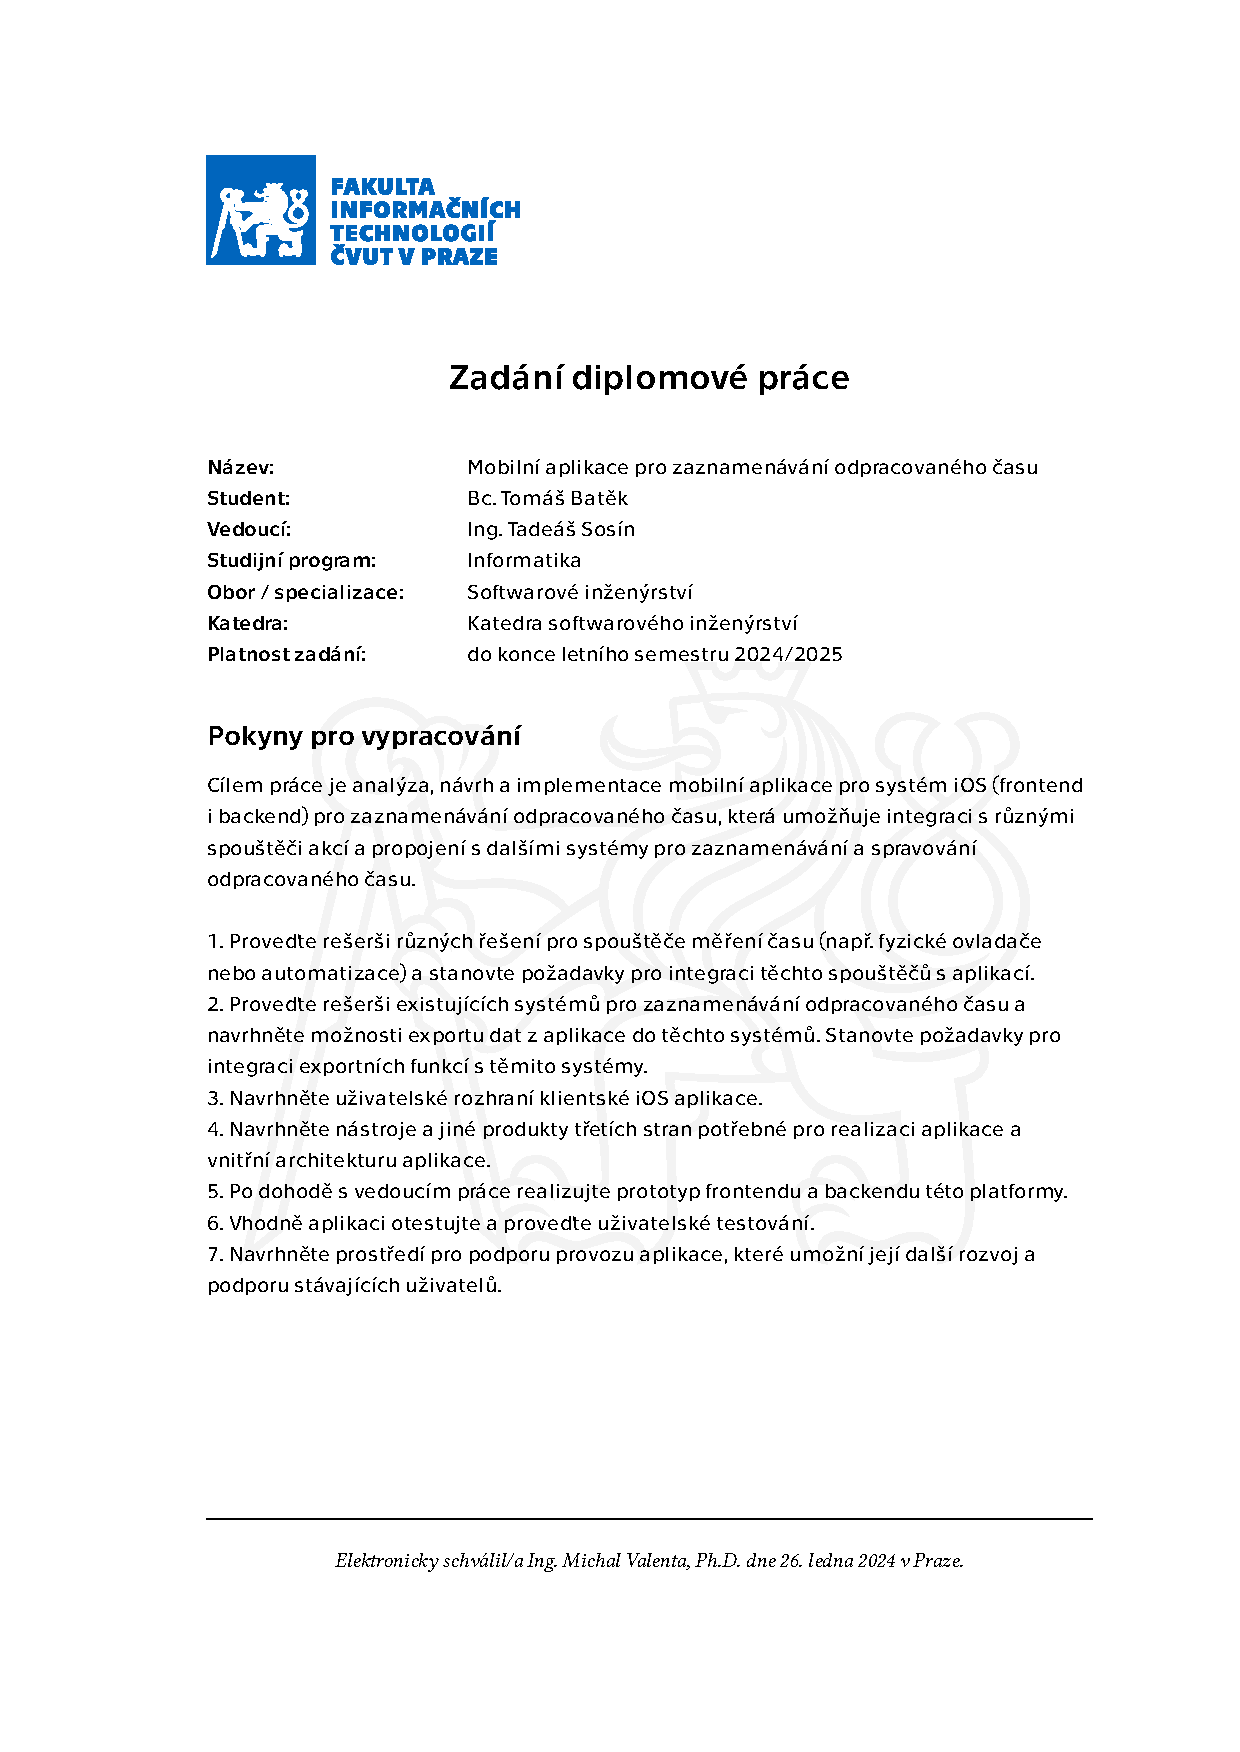
\includepdf{assignment-include.pdf} % replace that file with your thesis assignment provided by study office

\thispagestyle{empty}\cleardoublepage\maketitle % do not remove these three commands

\imprintpage % do not remove this command

\tableofcontents % do not remove this command
%%%%%%%%%%%%%%%%%%%%%%
% list of other contents: figures, tables, code listings, algorithms, etc.
% add/remove commands accordingly
%%%%%%%%%%%%%%%%%%%%%%
\listoffigures % list of figures
\begingroup
\let\clearpage\relax
%\listoftables % list of tables
% \lstlistoflistings % list of source code listings generated by the listings package
\listoflistings % list of source code listings generated by the minted package
\endgroup
%%%%%%%%%%%%%%%%%%%%%%
% list of other contents END
%%%%%%%%%%%%%%%%%%%%%%

%%%%%%%%%%%%%%%%%%%
% ACKNOWLEDGMENT
% FILL IN / MODIFY
% This is a place to thank people for helping you. It is common to thank your supervisor.
%%%%%%%%%%%%%%%%%%%
\begin{acknowledgmentpage}
	Chtěl bych poděkovat svému vedoucímu práce, panu Ing. Tadeášovi Sosínovi, za pomoc a~vstřícnost během tvorby práce. Také bych chtěl poděkovat své rodině za podporu při studiu.
\end{acknowledgmentpage} 
%%%%%%%%%%%%%%%%%%%
% ACKNOWLEDGMENT END
%%%%%%%%%%%%%%%%%%%


%%%%%%%%%%%%%%%%%%%
% DECLARATION
% FILL IN / MODIFY
%%%%%%%%%%%%%%%%%%%
% INSTRUCTIONS
% ENG: choose one of approved texts of the declaration. DO NOT CREATE YOUR OWN. Find the approved texts at https://courses.fit.cvut.cz/SFE/download/index.html#_documents (document Declaration for FT in English)
% CZE/SLO: Vyberte jedno z fakultou schvalenych prohlaseni. NEVKLADEJTE VLASTNI TEXT. Schvalena prohlaseni najdete zde: https://courses.fit.cvut.cz/SZZ/dokumenty/index.html#_dokumenty (prohlášení do ZP)
\begin{declarationpage}
Prohlašuji, že jsem předloženou práci vypracoval samostatně a~že jsem uvedl veškeré použité informační zdroje v~souladu s~Metodickým pokynem o~dodržování etických principů při přípravě vysokoškolských závěrečných prací.

Beru na vědomí, že se na moji práci vztahují práva a~povinnosti vyplývající ze zákona č.~121/2000~Sb., autorského zákona, ve znění pozdějších předpisů, zejména skutečnost, že České vysoké učení technické v~Praze má právo na uzavření licenční smlouvy o~užití této práce jako školního díla podle §60 odst.~1 citovaného zákona.
\end{declarationpage}
%%%%%%%%%%%%%%%%%%%
% DECLARATION END
%%%%%%%%%%%%%%%%%%%

\printabstractpage % do not remove this command

%%%%%%%%%%%%%%%%%%%
% SUMMARY
% FILL IN / MODIFY
% OR REMOVE ENTIRELY (upon agreement with your supervisor)
% (appropriate to remove in most theses)
%%%%%%%%%%%%%%%%%%%
% \begin{summarypage}
% \section*{Summary section}
% 
% \lipsum[1][1-8]
% 
% \section*{Summary section}
% 
% \lipsum[2][1-6]
% 
% \section*{Summary section}
% 
% \lipsum[3]
% 
% \section*{Summary section}
% 
% \lipsum[2]
% 
% \section*{Summary section}
% 
% \lipsum[1][1-8] Lorem lorem lorem.
% \end{summarypage}
%%%%%%%%%%%%%%%%%%%
% SUMMARY END
%%%%%%%%%%%%%%%%%%%

%%%%%%%%%%%%%%%%%%%
% ABBREVIATIONS
% FILL IN / MODIFY
% OR REMOVE ENTIRELY
% List the abbreviations in lexicography order.
%%%%%%%%%%%%%%%%%%%
\chapter{Seznam zkratek}
	
\begin{tabular}{rl}
API & Application Programming Interface\\
BLE & Bluetooth Low Energy\\
SDK & Software Development Kit\\
UI & User Interface\\
BaaS & Backend as a Service\\
DBaaS & Database as a Service\\
CSV & Comma-Separated Values\\
JSON & JavaScript Object Notation\\
URL & Uniform Resource Locator\\
IP & Internet Protocol\\
HTTP & Hypertext Transfer Protocol\\
DTO & Data transfer object\\
OS & Operating System\\
\end{tabular}
%%%%%%%%%%%%%%%%%%%
% ABBREVIATIONS END
%%%%%%%%%%%%%%%%%%%

\mainmatter\mainmatterinit % do not remove these two commands

%%%%%%%%%%%%%%%%%%%
% THE THESIS
% MODIFY ANYTHING BELOW THIS LINE
%%%%%%%%%%%%%%%%%%%

% Do not forget to include Introduction

\graphicspath{ {./images} }

%---------------------------------------------------------------
\chapter*{Úvod}
%---------------------------------------------------------------
\addcontentsline{toc}{chapter}{Úvod}
\setcounter{page}{1}
\markboth{Úvod}{Úvod}

Zaznamenávání a~správa odpracovaného času je problematikou, která může sloužit velkému množství uživatelů různých odvětví zaměstnání. Ať už se jedná o~sledování pracovních hodin za účelem fakturace, za účelem sledování docházky, nebo za účelem analýzy produktivity, jedná se o~službu, kterou vyžaduje a~používá velké množství zaměstnanců a~zaměstnavatelů.

Vzhledem k~tomu, že je poptávka po službě zprostředkovávající měření a~správu odpracovaného času poměrně vysoká, existuje řada řešení, které se tuto službu snaží s~různými přístupy a~funkcionalitami nabízet. Mohou proto nastávat situace, kdy budou uživatelé potřebovat nějakou formu integračního prvku, který bude moct propojovat více řešení a~přístupů, jak odpracovaný čas měřit a~jak ho analyzovat. 

Tato práce nabízí implementaci vlastního řešení aplikace pro měření a~správu odpracovaného času a~jako přidanou hodnotu analyzuje možnosti integrace se spouštěči měření času (fyzické ovladače, automatizace, \dots), možnosti integrace s~existujícími systémy pro správu odpracovaného času, poté navrhuje, jaké typy integrací implementovat, a~v~realizované aplikaci tyto integrace nabízí.

Podkladem pro funkcionality realizované aplikace je analýza existujících řešení a~přístupů pro měření správu času, analýza možností pro integraci a~návrh používání aplikace z~výstupů analýzy.

Implementace aplikace zhotovená v~rámci této práce nemá šanci se vyrovnat existujícím aplikacím řešícím problematiku měření a~správy času, které mají mnohem větší časové a~finanční rozpočty a~stojí za nimi roky vývoje velkých týmů. Má ale šanci poskytnout základ aplikace, která mimo samotnou možnost měření a~správy odpracovaného času dokáže nabídnout i~nějaké vhodné formy integrace se spouštěči měření a~těmito zmíněnými existujícími aplikacemi. Na tomto základu poté může být navázáno dalším úsilím, které funkcionality a~možnosti integrace aplikace rozšíří. 

Mimo poskytnutí základu integrační aplikace pro měření a~správu odpracovaného času má také tato práce potenciál nabídnout seznámení s~aktuálními moderními přístupy vývoje mobilních aplikací a~s~nástroji k~tomu potřebnými.

%---------------------------------------------------------------
\chapter{Cíl práce}
%---------------------------------------------------------------

Hlavním cílem diplomové práce je analýza, návrh a~implementace mobilní aplikace pro systém iOS (frontend i~backend) pro zaznamenávání odpracovaného času, která umožňuje integraci s~různými spouštěči akcí a~propojení s~dalšími systémy pro zaznamenávání a~spravování odpracovaného času. V~rámci návrhu je cílem navrhnout vhodné technické řešení pro implementaci aplikace, funkcionality aplikace a~jejich uživatelské rozhraní a~tohoto návrhu se poté při realizaci aplikace držet. Následně je cílem práce realizované řešení vhodně otestovat a~provést uživatelské testování. 

Vedlejším cílem realizovaného řešení je flexibilita a~rozšiřovatelnost technické implementace aplikace. Jelikož základ integrační aplikace pro měření a~správu odpracovaného času, který tato práce realizuje, má široké možnosti budoucího rozšíření, ať už o~aplikace pro další platformy (Android, Web, \dots), tak o~další funkcionality (propojení s~mnohými dalšími řešeními), tak je přinejmenším vhodné, aby na tyto rozšíření byla co nejlepším způsobem připravena.

Výsledky diplomové práce budou přínosné pro potenciální budoucí uživatele nové realizované platformy, ale také pro čtenáře, kteří se chtějí seznámit s~technickým přístupem řešení, které bylo v~této práci zvoleno, proč bylo zvoleno, jaké byly alternativy a~jaké je poté v~závěru zhodnocení tohoto přístupu. Vývoj mobilních aplikací je~stále rostoucím průmyslem, který je stále ve fázi objevování nových přístupů a~řešení, a~tato práce má potenciál do něj přispět zkušenostmi, které byly při její realizaci získány.

%---------------------------------------------------------------
\chapter{Analýza}
%---------------------------------------------------------------

Tato kapitola rozebírá, k~čemu slouží zaznamenávání odpracovaného času. Poté popisuje možnosti, které umožňují měření času spouštět a také se věnuje příkladům řešení, která již pro zaznamenávání odpracovaného času existují, a jaké jsou možnosti propojení s~těmito řešeními. V~dalších sekcích se poté obecně zaměřuje na vývoj aplikací pro mobilní platformu iOS včetně možností multi-platformního a cross-platformního vývoje.

%---------------------------------------------------------------
\section{Zaznamenávání odpracovaného času}
%---------------------------------------------------------------

Zaznamenávání odpracovaného času může být potřeba z~několika různých důvodů, buď z~pohledu jednotlivce, nebo z~pohledu spolupráce v~nějakém týmu. Mezi tyto důvody může patřit například:
\begin{itemize}
\item\textbf{Sledování pracovních hodin:} Pomáhá zaměstnancům a podnikům sledovat, kolik času strávili na různých úkolech, projektů a aktivitách během pracovní doby. To může být užitečné pro sledování produktivity, hodnocení efektivity práce a plánování rozpočtu času.
\item\textbf{Fakturace a účtování:} Pro profesionály a firmy, které účtují za své služby na základě odpracovaného času, umožňuje zaznamenávání snadné sledování času stráveného na jednotlivých projektech a klientech pro účely fakturace.
\item\textbf{Analýza produktivity:} Poskytuje data a statistiky o~tom, jaký čas je věnován různým úkolům a projektům. To umožňuje identifikovat trendy v~pracovních návycích, optimalizovat časové plánování a zlepšit efektivitu práce.
\item\textbf{Správa projektů:} Pomáhá organizovat časové údaje spojené s~různými projekty a úkoly, což usnadňuje plánování, delegování a monitorování pokroku.
\item\textbf{Transparentnost a komunikace:} Pro týmy umožňuje transparentně sdílet informace o~čase stráveném na různých aktivitách, což podporuje spolupráci a komunikaci v~rámci týmu.
\end{itemize}

Celkově zaznamenávání slouží k~lepšímu řízení času, sledování produktivity a optimalizaci využití pracovního času pro jednotlivce i~organizace.

\begin{figure}[h]
	\centering
	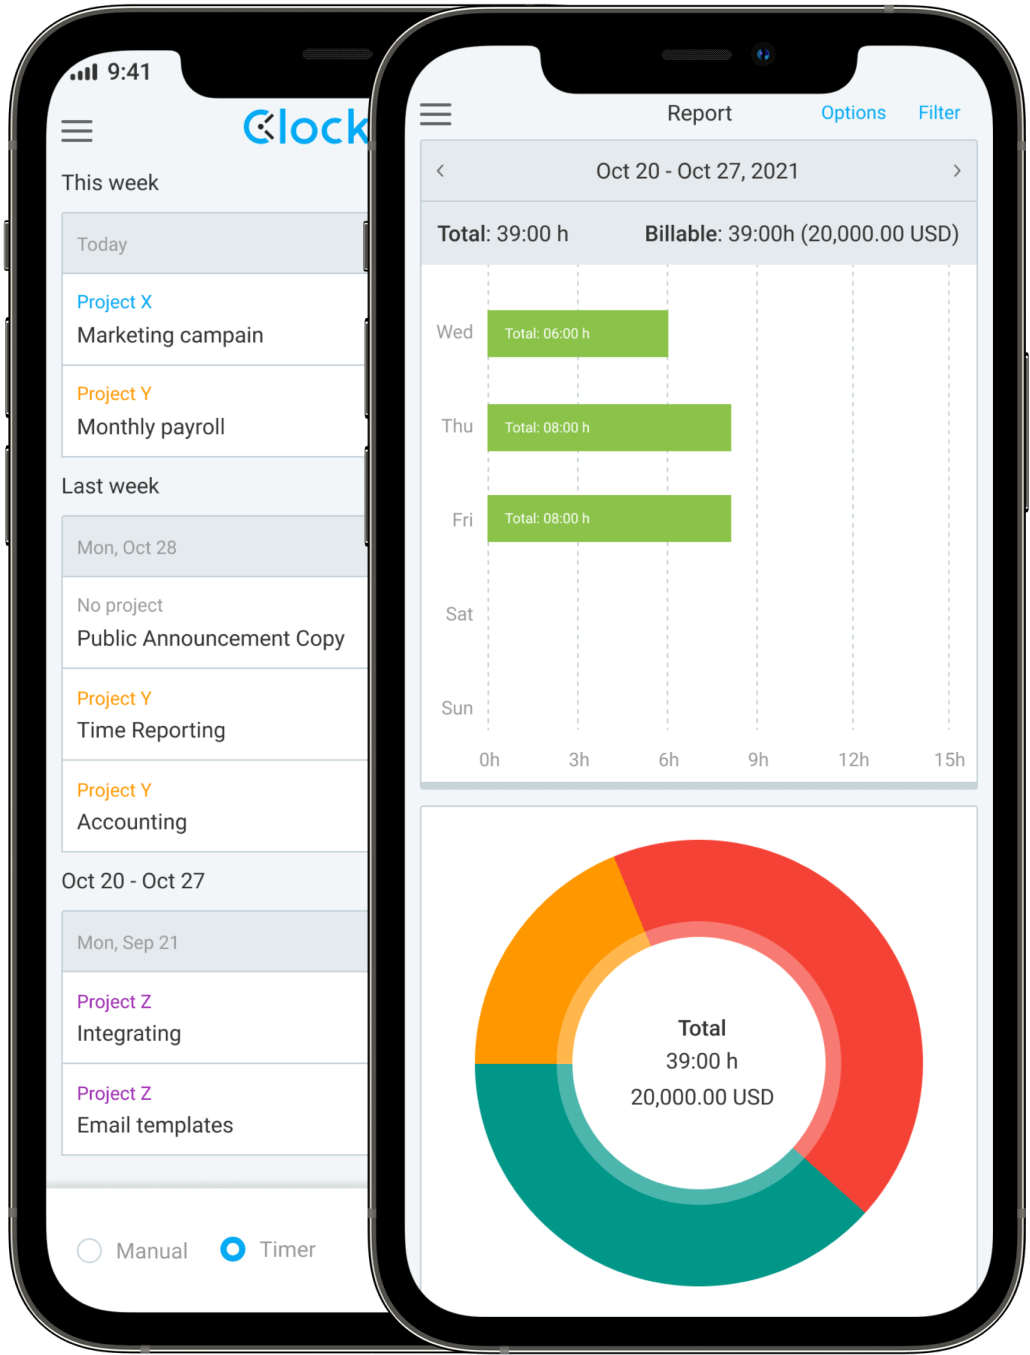
\includegraphics[width=10cm]{clockify-ios.png}
	\caption{Clockify – iOS aplikace pro měření času \cite{clockify-ios}}
	\label{fig:clockify-ios}
\end{figure}

%---------------------------------------------------------------
\section{Spouštěče měření času}\label{tracking-triggers}
%---------------------------------------------------------------

Jedním z~cílů této práce je prozkoumat různá řešení pro spouštěče měření času. Nejjednodušším spouštěčem je samozřejmě ruční zapnutí nějaké formy časovače v~samotné aplikaci, která pro měření času slouží. To ale umí kdejaké již existující řešení a přidanou hodnotou této práce by měly být nějaké možnosti, jak spouštění uživateli ulehčit. Tyto možnosti se dají rozdělit do dvou kategorií – fyzické a softwarové.

%---------------------------------------------------------------
\subsection{Fyzické}
%---------------------------------------------------------------

Za fyzické spouštěče měření času lze považovat jakoukoli formu fyzického ovladače, kterou může uživatel nějak ovládat a tím spouštět časovač měření času.

Častým typem fyzického spouštěče je nějaká forma takzvaného platónského tělesa (krychle, osmistěn, dvanáctistěn, atd.), které může uživatel otáčet. Podle toho, na kterou stranu ho položí, tak se spustí časovač s danými parametry. Různé strany tělesa mohou sloužit například pro identifikování toho, na kterém projektu uživatel zrovna pracuje.

Mezi fyzické spouštěče patří například tyto produkty:
\begin{itemize}
\item\textbf{TIMEFLIP:} Dvanáctistěnné těleso, na které si uživatel může nalepovat cokoli, co bude identifikovat odpracovaný čas. Těleso se propojí s~mobilní aplikací, která poté spravuje naměřený čas. \cite{timeflip}
\item\textbf{TIMEULAR:} Stejný princip jako \emph{TIMEFLIP}, akorát používá osmistěnné těleso. Jednotlivé strany jdou také přizpůsobovat nálepkami. \cite{timeular}
\item\textbf{timeBuzzer:} Fyzické tlačítko, které lze umístit na stůl a zapojit do počítače. Stisknutí tlačítka otevře okno měřící aplikace, otočením tlačítka lze vybrat projekt a opětovným stisknutím se začne daný projekt měřit. \cite{timebuzzer}
\end{itemize}

\begin{figure}[h]
	\centering
	\begin{subfigure}[b]{5.2cm}
		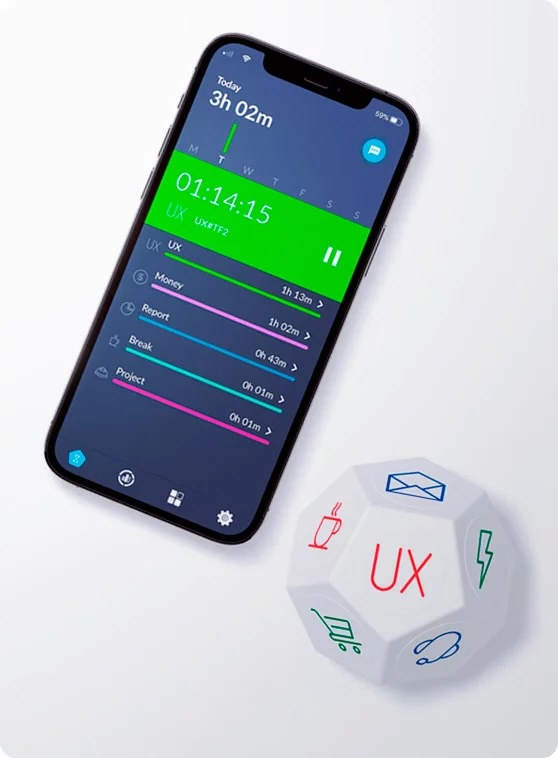
\includegraphics[width=5.2cm]{timeflip.jpeg}
		\caption{TIMEFLIP – Kostka a aplikace \cite{timeflip}}
		\label{pic:timeflip}
	\end{subfigure}
	\hspace{2cm}
	\begin{subfigure}[b]{7cm}
		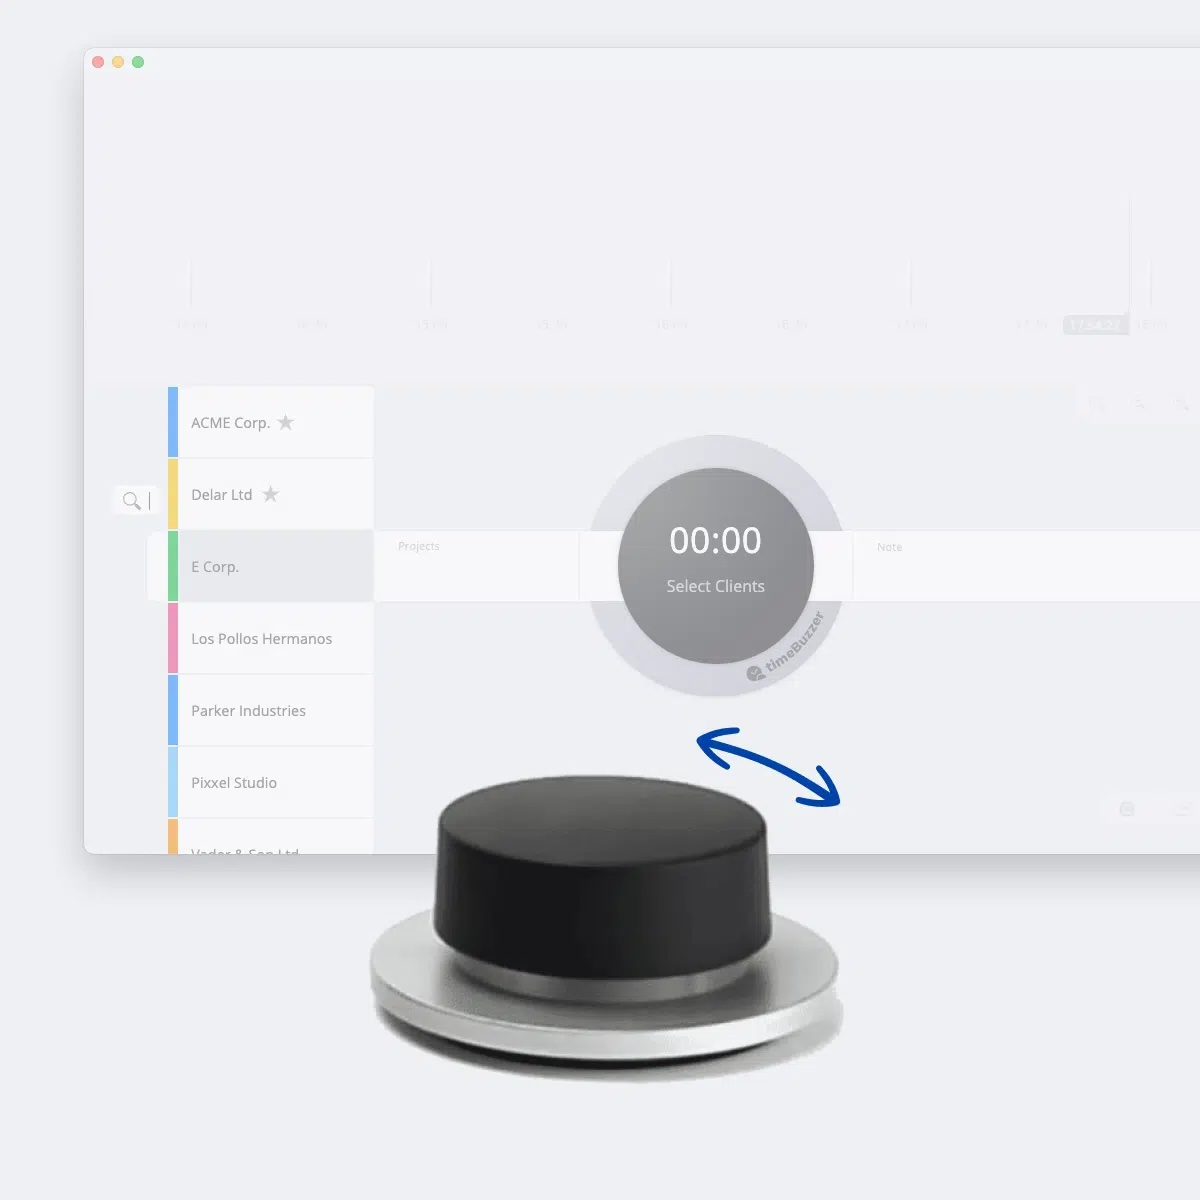
\includegraphics[width=7cm]{timebuzzer.jpeg}
		\caption{timeBuzzer – tlačítko a aplikace \cite{timebuzzer}}
		\label{pic:timebuzzer}
	\end{subfigure}
\end{figure}

Všechny ze zmíněných produktů poskytují veřejné API pro aplikace, se kterými komunikují \cite{timeflip-api} \cite{timeular-api} \cite{timebuzzer-api}. Pokud by tedy bylo potřeba produkty propojit s~vlastní aplikací, která by mohla naměřený čas spravovat, bylo by potřeba, aby aplikace komunikovala s~těmito nástroji. Pořád by byl potřeba prostředník, kterým by byla aplikace daného produktu. Výjimkou je v~těchto produktech pouze \emph{TIMEFLIP}, který poskytuje veřejný protokol pro BLE komunikaci \cite{timeflip-ble-api}. Tento produkt by tedy mohl komunikovat s~novou aplikací napřímo.

Pokud by nová aplikace měla umožňovat budoucí propojení s~jakýmkoli dalším hardwarovým produktem, tak by také měla poskytovat veřejné API, které by takovou komunikaci umožňovalo. Vývoj takových produktů by mohl být předmětem návrhu pro budoucí vylepšení aplikace.

%---------------------------------------------------------------
\subsection{Softwarové}\label{software-tracking-triggers}
%---------------------------------------------------------------

Za softwarové spouštěče měření času lze považovat určité formy integrace a automatizace v~rámci zařízení, na kterém aplikace běží. V~případě aplikace na platformě iOS to mohou být následující možnosti:
\begin{itemize}
\item\textbf{Automatizace podle polohy:} Aplikace by mohla reagovat na polohu uživatele a spouštět nebo vypínat časovač na základně informace, kde se uživatel nachází. Uživatel by si mohl například nastavit určitá místa, kde by chtěl, aby se automaticky spustil časovač. Mohl by se zapnout přímo s~konkrétními přednastavenými parametry (projekt, klient, \dots), nebo by se jen mohlo ukázat upozornění, aby si uživatel časovač zapnul sám, s~parametry, které zadá. Podobně by aplikace mohla reagovat i na opuštění nějakého místa – například pokud uživatel opustí místo, které má označeno jako práci, tak by dostal upozornění, zda si nechce vypnout časovač.
\item\textbf{Automatizace podle času:} Jednoduchá forma automatizace by mohla fungovat na základě času. V~přednastavených časech by se mohl zapnout nebo vypnout časovač s~danými parametry, nebo by aplikace mohla uživatele jen upozornit.
\item\textbf{Automatizace podle kalendáře:} Užitečná by také mohla být integrace s~kalendářem uživatele. Podle naplánovaných událostí by se časovač mohl automaticky zapínat, přepínat, nebo vypínat, s~parametry z~kalendáře. Nebo opět pouze uživatele upozornit, zda si kvůli nějaké události nechce měření času aktualizovat.
\item\textbf{Automatizace podle režimu soustředění:} Systém iOS umožňuje od verze 15.0 uživatelům používat takzvané \emph{Režimy soustředění} \cite{ios-focus-modes}. Uživatel si může konfigurovat různé režimy a nastavovat, jaké mu v~tomto režimu budou chodit upozornění, jaké aplikace může používat, kdo mu může volat, apod. Od iOS verze 16 také Apple umožňuje vývojářům přizpůsobovat chování aplikace podle toho, jaký režim soustředění je zapnutý \cite{ios-focus-modes-adjustment}. Toho by se dalo vhodně využít například tak, že by se mohl automaticky spouštět časovač (nebo by uživatel mohl být upozorněn) podle toho, do jakého režimu soustředění se uživatel právě přepnul.
\item\textbf{Automatizace pomocí zkratek:} Apple nabízí uživatelům s~iOS verze 13.0 nebo novější aplikaci \emph{Zkratky} \cite{ios-shortcuts-app}, která umožňuje tvorbu vlastních automatizujících procesů \cite{ios-shortcuts}. Tento způsob automatizace umožňuje uživatelům i~vývojářům velkou míru přizpůsobitelnosti – zkratky jdou propojovat s~dalšími aplikacemi, s~hlasovým asistentem a s~mnoha různými akcemi. Všechny předchozí způsoby automatizace jdou také nějakým způsobem vytvořit pomocí zkratek. \cite{ios-shortcuts-developer}
\end{itemize}

%---------------------------------------------------------------
\section{Existující systémy pro měření a správu odpracovaného času}\label{existing-tracking-solutions}
%---------------------------------------------------------------

Systémů pro měření a správu odpracovaného času existuje mnoho. Existuje dokonce několik různých článků o~tom, které systémy jsou nejlepší a jaké je jejich srovnání \cite{forbes-tracking-apps-article} \cite{zapier-tracking-apps-article}. Následující výběr příkladů je učiněn podle těchto článků, podle osobní preference a podle počtu stažení na iOS platformě. U~každého příkladu jsou také rozebrány možnosti importu dat, od kterých se mohou odvíjet požadavky na export dat z~nové aplikace.

%---------------------------------------------------------------
\subsection{Clockify}
%---------------------------------------------------------------

Clockify je jednoduchá a rozšířená aplikace primárně určená pro měření a správu odpracovaného času. Mobilní aplikace má více než 1 milion stažení \cite{clockify-app-magic} a celý systém používají miliony lidí \cite{clockify-customers}. 

V článku Forbes je hodnocena jako celkově nejlepší aplikace pro měření času pro rok 2024. Má široké spektrum funkcionalit – umožňuje měření a správu času pro různé projekty, klienty a zařízení. Mimo měření času nabízí také sledování prezence pro mzdy a účetnictví, optimalizaci produktivity zaměstnanců, měření vykazovatelného času a sdílení pokroku na projektech s~klienty. \cite{forbes-tracking-apps-article}

Clockify nabízí aplikace pro mnoho platforem: Desktopovou aplikaci pro Mac, Windows a Linux, doplněk webového prohlížeče pro Chrome, Firefox a Edge, mobilní aplikaci pro iOS a Android a nakonec sdílené Kioskové řešení, na kterém si uživatelé mohou zapisovat příchody, přestávky a další. \cite{clockify-apps}

V~základní variantě je používání aplikace zdarma. Clockify ale nabízí i~placené plány, které nabízí přidané funkce, jako audity naměřených časů, používání přestávek a další. Tyto placené plány mohou stát od \$3.99 měsíčně za uživatele až po \$11.99 měsíčně za uživatele. \cite{clockify-pricing} 

\begin{figure}[p]
	\centering
	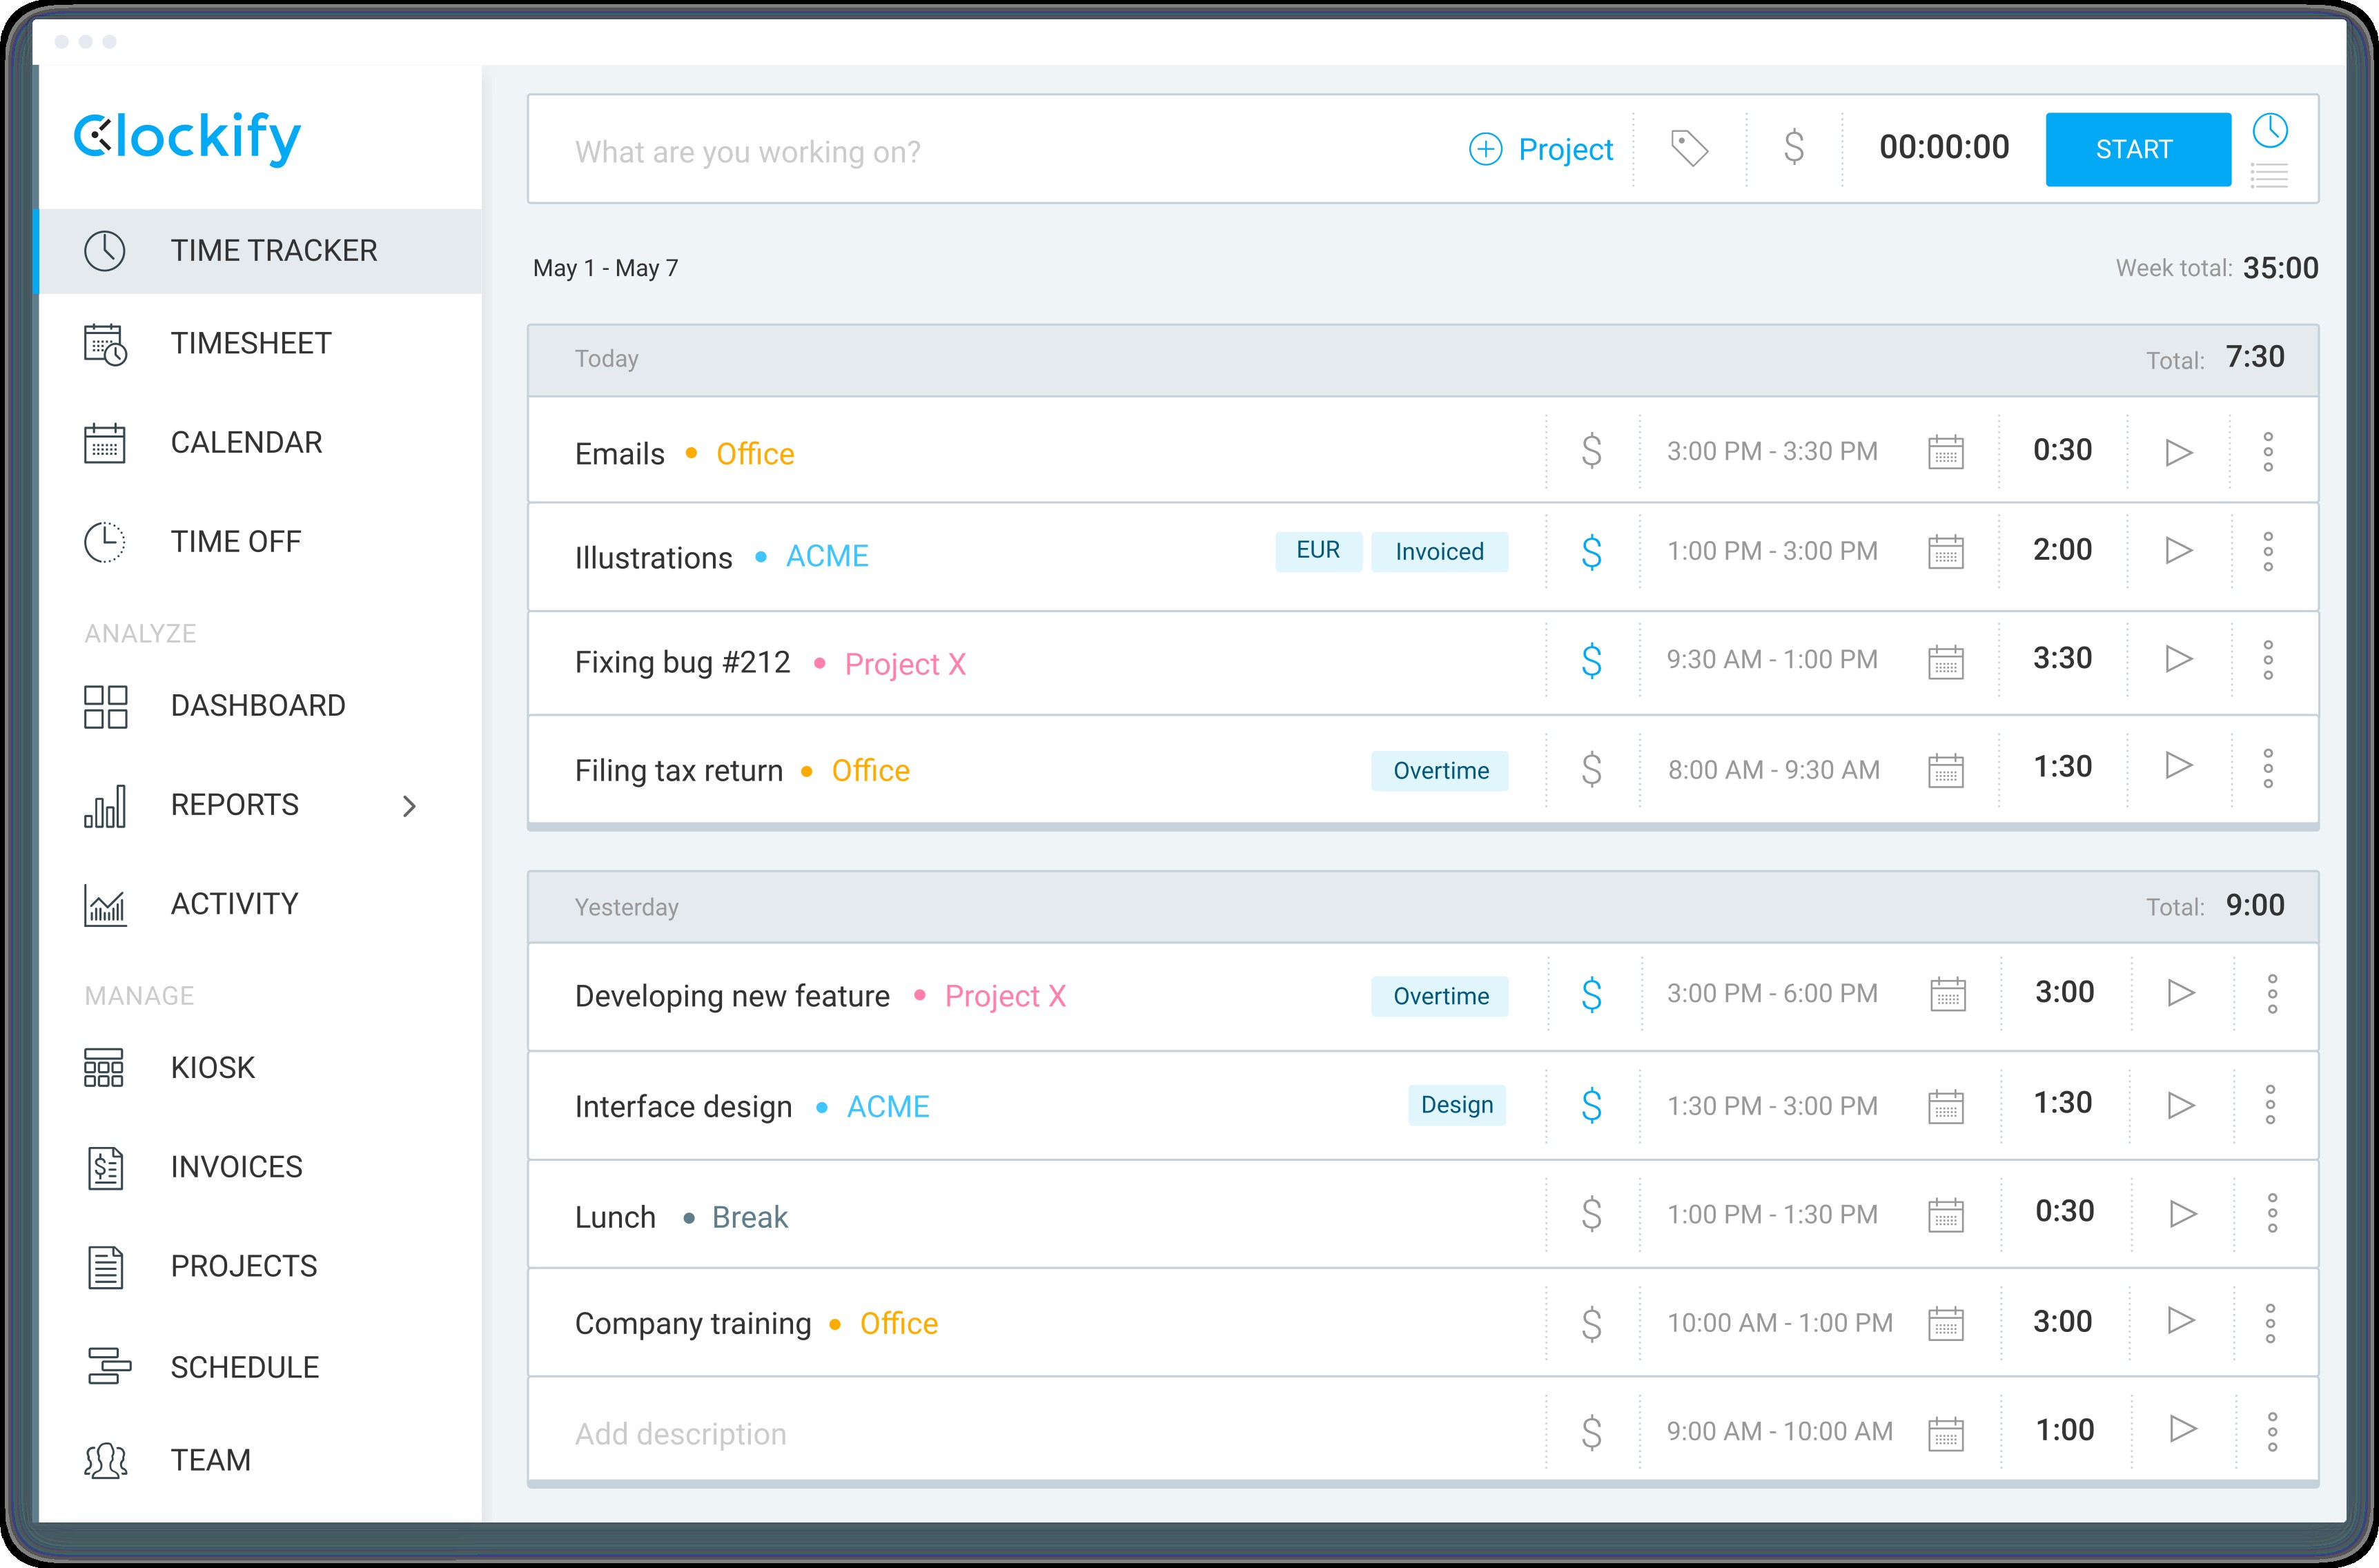
\includegraphics[width=0.9\textwidth]{clockify-timer.jpg}
	\caption{Časovač na měření času v~aplikaci Clockify \cite{clockify-features}}
	\label{fig:clockify-timer}
	\vspace{1cm}
	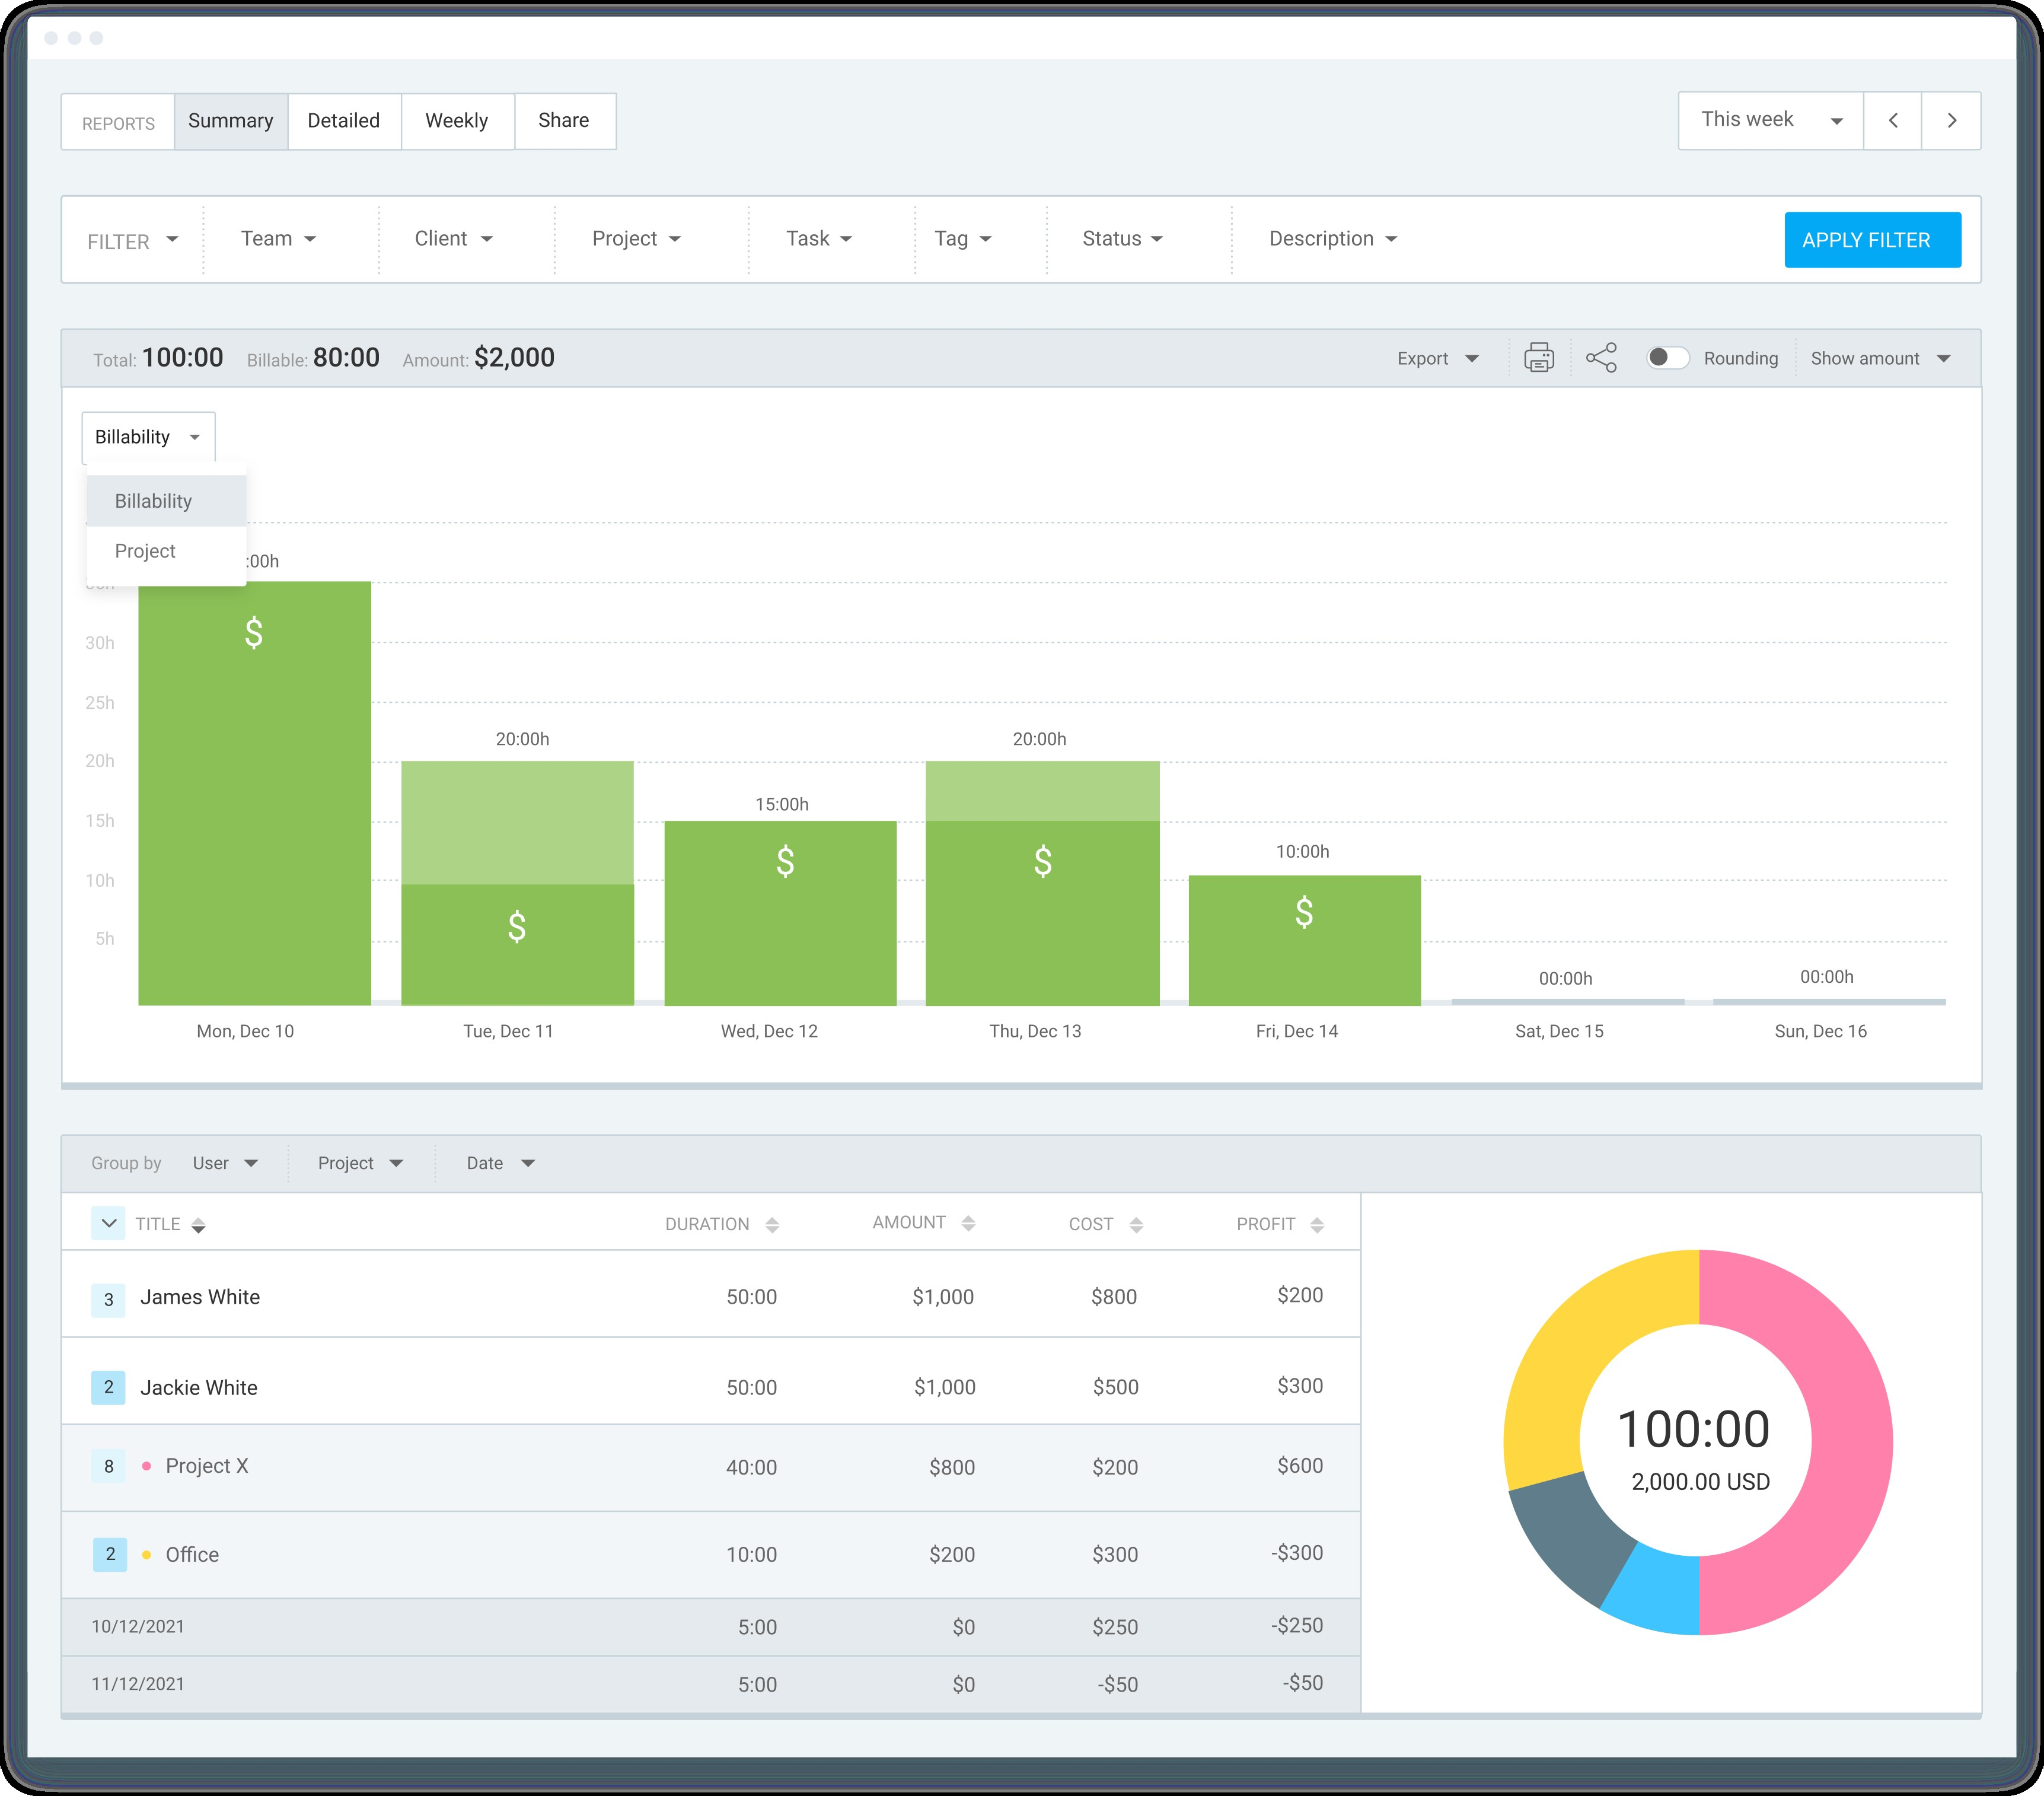
\includegraphics[width=0.9\textwidth]{clockify-report.jpg}
	\caption{Reporty v~aplikaci Clockify \cite{clockify-features}}
	\label{fig:clockify-report}
\end{figure}

Clockify nabízí dobře zdokumentované API pro své služby \cite{clockify-api}. Napojení na funkce systému lze tedy jednoduše udělat i~z~vlastního řešení. Do Clockify lze také data importovat z~CSV tabulek, jsou-li data vhodně naformátována \cite{clockify-import-timesheets}.

Mezi nevýhody systému Clockify Forbes uvádí, že projekty nejdou označit jako dokončené, a že shrnující reporty mohou být zpočátku matoucí. Celkově Clockify ale vnímá jako nejlepší řešení pro pokrytí celé škály funkcionalit.

Na obrázku \ref{fig:clockify-timer} je vidět hlavní obrazovka ve webové verzi aplikace – časovač. Uživatel si zde může časovat ručně zapnout a vypnout, přidělit projekt, přidat značky, označit vykazovatelnost a přidat popisek. Také má možnost přidat odpracovaný čas ručně, tedy ne pomocí časovače. K~tomu stačí jen napsat čas začátku a konce. Pod ovládacím panelem časovače potom uživatel vidí seznam svých již zadaných časových záznamů, které zde může jakkoli upravovat.

Dále je na obrázku \ref{fig:clockify-report} vidět obrazovka určená pro reporty. Uživatel si zde může vybrat časový úsek, pro který chce report vypracovat, a může si nastavit filtry, podle kterých chce časové vstupy filtrovat (tým, klient, projekt, úkol, značka, stav a popisek). Po aplikování filtru poté uživatel uvidí report své práce vyhovující zadaným parametrům, který si může exportovat ve formátech PDF, CSV a Excel.

%---------------------------------------------------------------
\subsection{Toggl Track}
%---------------------------------------------------------------

Toggl track je další poměrně rozšířená aplikace pro měření a správu času. Na platformě iOS má více než 1 milion stažení \cite{toggl-track-app-magic}. 

Forbes tuto aplikaci považuje za nejlepší pro malé týmy, protože nabízí plán zdarma pro týmy do 5 uživatelů a nabízí neomezený počet klientů a projektů. \cite{forbes-tracking-apps-article}

Aplikace nabízí určitou formu automatické detekce toho, že uživatel nemá zapnutý časovač, i~když pracuje, nebo automatickou detekci naopak toho, že uživatel už nepracuje, ale časovač má zapnutý. Aplikace nabízí detailní denní, týdenní a měsíční reporty.

Toggl Track také pokrývá více platforem: Webovou aplikací, mobilní aplikací pro iOS a Android a desktopovou aplikací pro Windows a Mac. \cite{toggl-track}

\begin{figure}[h]
	\centering
	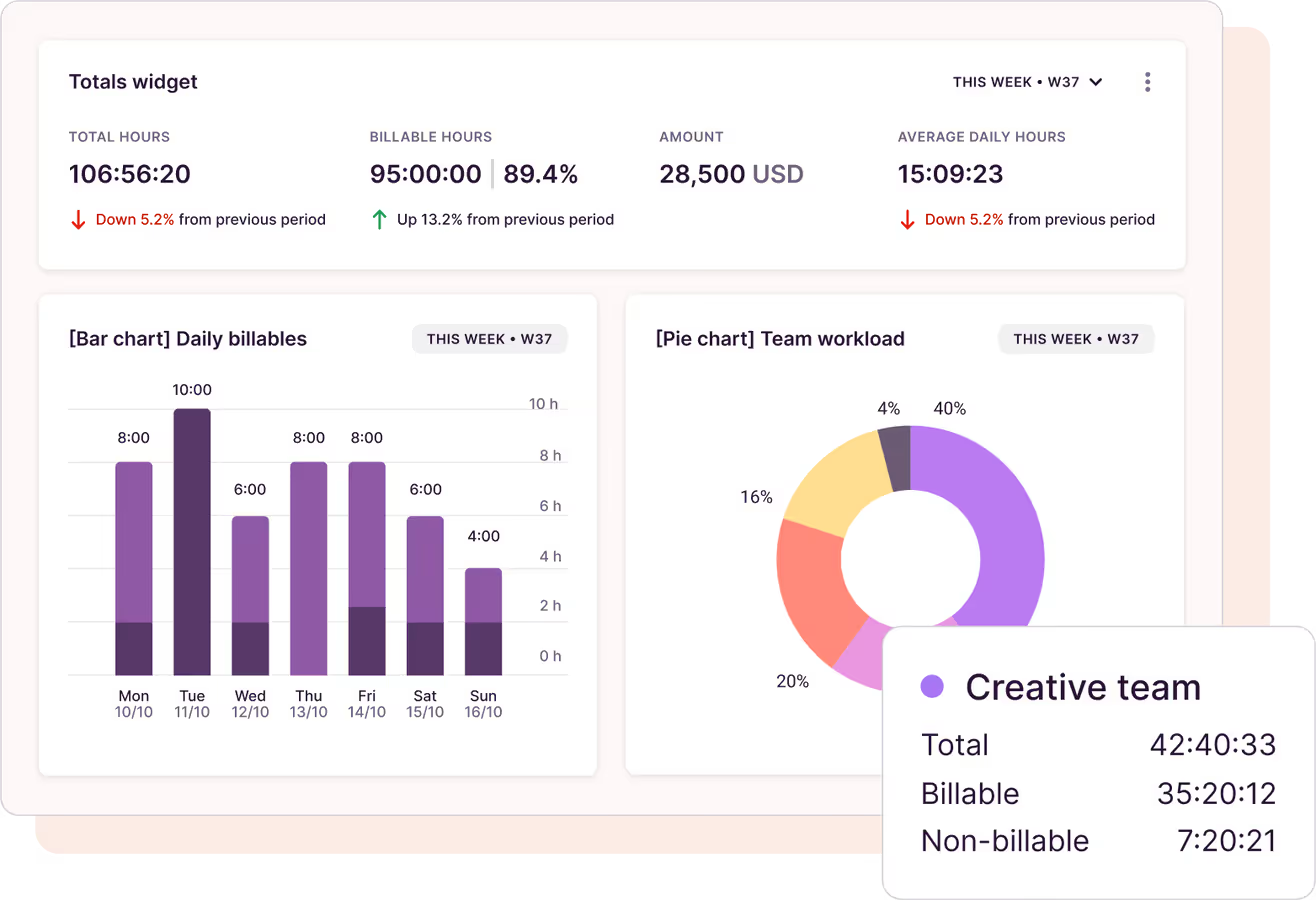
\includegraphics[width=\textwidth]{toggl-track.png}
	\caption{Aplikace Toggl Track \cite{toggl-track}}
\end{figure}

Toggl Track také nabízí možnost importu dat z~CSV tabulky, ve velmi podobném formátu jako Clockify \cite{toggl-track-import-csv}. A stejně jako Clockify nabízí vlastní otevřené API \cite{toggl-track-api}.

%---------------------------------------------------------------
\subsection{Deputy}\label{deputy}
%---------------------------------------------------------------

Deputy je další aplikací, která umožňuje měření a správu odpracovaného času. Jejím hlavním účelem je však plánování směn zaměstnanců. Je uvedena jako jeden z~příkladů proto, aby šlo nahlédnout na problém měření času i~z~jiného úhlu, než striktně měření času primárně za účelem vykazování, fakturování nebo analýzy efektivity. Je také velice rozšířenou aplikací – počty stažení na mobilních telefonech překračují 5 milionů \cite{deputy-app-magic}.

Právě plánování směn zaměstnanců je hlavním důvodem, proč Forbes tuto aplikaci ve svém seznamu zmiňuje. Aplikace totiž nabízí plánování neomezeného počtu směn za měsíc. Uživatelé se mohou přihlásit k~aplikacím pro plánování a pro prezenci zvlášť. I~neplacený plán umožňuje automatické plánování směn, což šetří čas manažerům. Toto plánování umožňuje i~započítání obědových pauz, přestávek a dalšího, přímo do plánu směn, podle příslušných zákonů.  \cite{forbes-tracking-apps-article}

Deputy nabízí aplikaci pro měření odpracovaného času pro mobilní platformy iOS a Android. 

\begin{figure}[h]
	\centering
	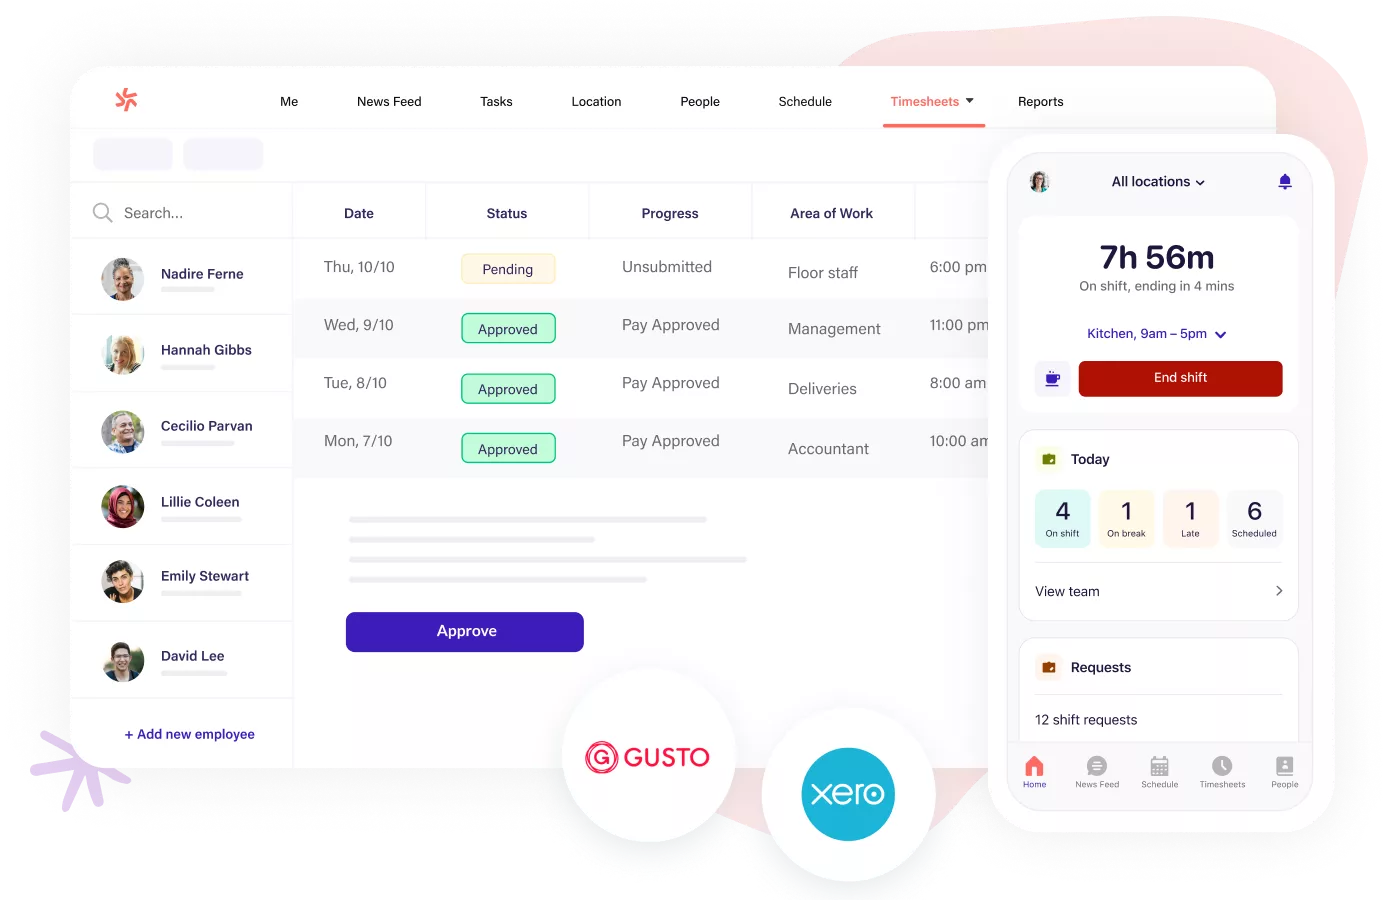
\includegraphics[width=\textwidth]{deputy.png}
	\caption{Aplikace Deputy \cite{deputy-time-tracking-app}}
\end{figure}

Stejně jako předchozí systémy, Deputy nabízí možnost importu dat z~CSV tabulky \cite{deputy-import-csv}. Vzhledem k~trochu jinému byznysovému modelu této aplikace ale tyto data musí narozdíl od předchozích systémů obsahovat dodatečná data, jako místo, pauzy na oběd, a další. A ani u~této aplikace nechybí otevřené API \cite{deputy-api}.

%---------------------------------------------------------------
\section{Vývoj mobilních aplikací pro systém iOS}
%---------------------------------------------------------------

Tato sekce se věnuje několika klíčovým tématům souvisejícím s~vývojem aplikací pro zařízení s operačním systémem iOS. Tyto témata shrnuje a poskytuje tím základ pro diskuzi o~vývoji aplikací pro tento systém.

%---------------------------------------------------------------
\subsection{Historie a vývoj iOS platformy}
%---------------------------------------------------------------

Historie operačního systému iOS začala v~roce 2007, kdy byl představen a začal se prodávat první mobilní telefon od společnosti Apple, kterým byl iPhone. V~tomto telefonu byl od výroby nainstalován operační systém, který ještě v~tu dobu nenesl název \emph{iOS}, ale \emph{iPhone OS}. Název \emph{iOS} se začal používat až později od verze systému 4. Přestože z~dnešního pohledu chybělo v~systému mnoho funkcí, se kterými si dnes mobilní telefony spojujeme, jako možnost instalace aplikací třetích stran, tak to byl v~tu dobu velký posun. Věci jako \emph{Multitouch screen}, vizuální znázornění hlasové schránky, nebo integrace s~\emph{iTunes}, byly obrovskou výhodou. Mezi předinstalované aplikace patřil kalendář, fotky, fotoaparát, poznámky, prohlížeč webu \emph{Safari}, e-mailový klient, telefon a \emph{iPod} (který se později rozdělil na aplikace pro hudbu a aplikace pro videa).

\begin{figure}[h]
	\centering
	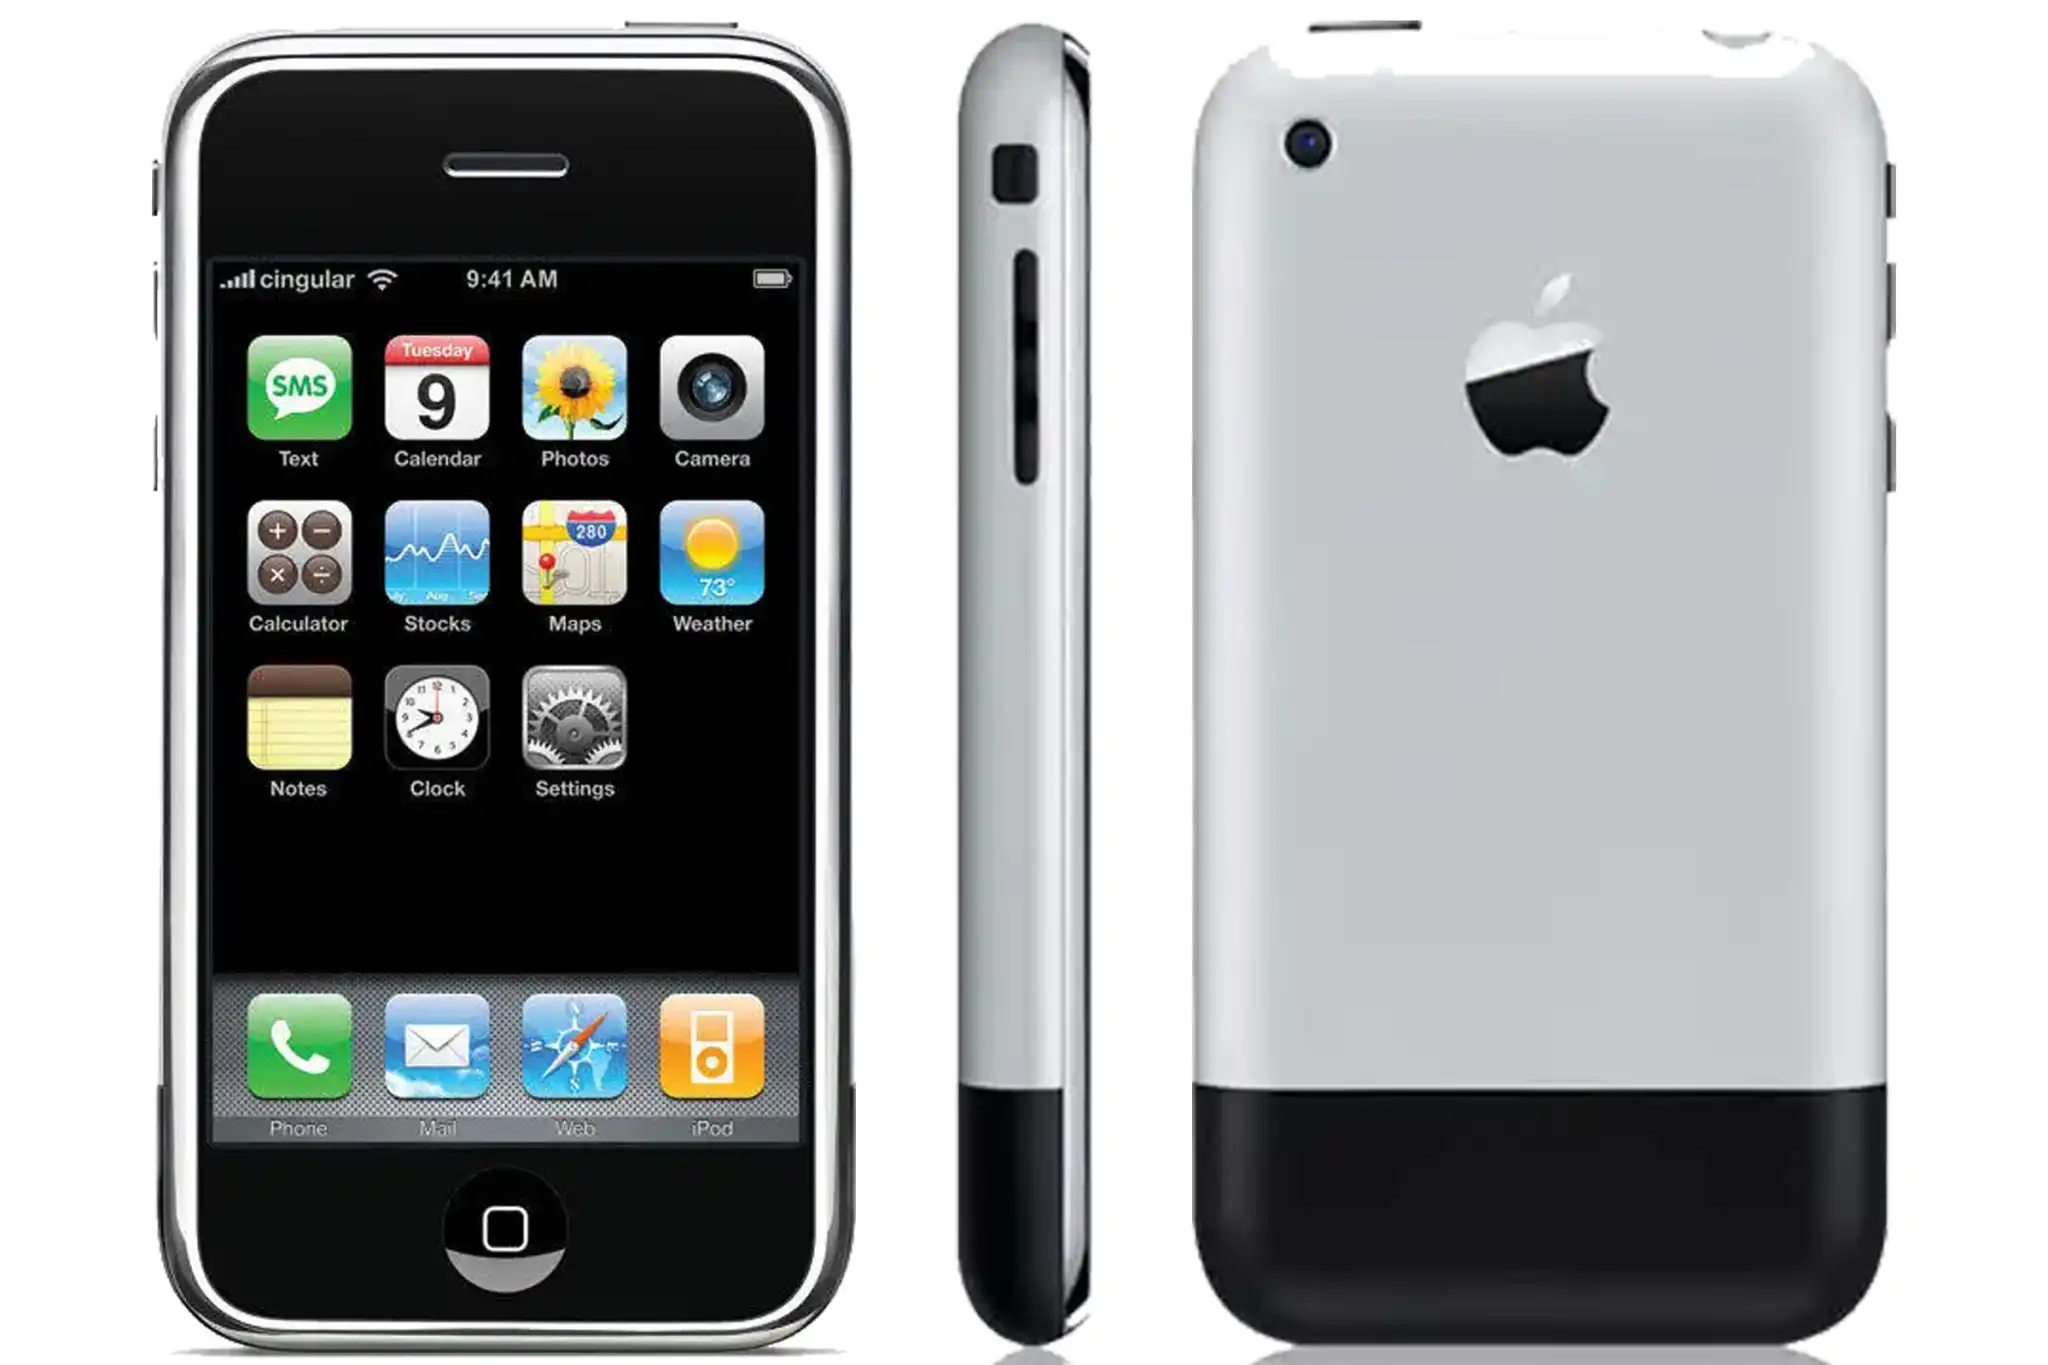
\includegraphics[width=10cm]{iphone.png}
	\caption{První model mobilního telefonu iPhone \cite{iphone-review}}
\end{figure}

O~rok později, v~roce 2008, byla představena nová generace mobilního telefonu s~názvem iPhone~3G, se kterým také vznikla nová verze operačního systému iOS (iPhone OS) 2.0. Hlavní novinkou této nové verze byl nový obchod s~aplikacemi třetích stran, \emph{App Store}. Až 500 aplikací bylo v~obchodě k~dispozici v~době, kdy byl zpřístupněn uživatelům.

V~roce 2009 poté s~novým iPhonem 3GS přišla verze iOS (iPhone OS) 3, která přinesla hlavně vylepšení, jako možnost používat kopírování a vkládání, vyhledávání přes \emph{Spotlight}, podporu MMS a možnost natáčet videa (do té doby iPhone uměl pouze pořizovat fotky). Také to byla první verze operačního systému, která fungovala i~na nových tabletech od společnosti Apple – na iPadech. První iPad byl představen v~roce 2010.

V~roce 2010 byl představen nový iPhone 4 a s~ním verze operačního systému 4. Od této verze se začal používat název \emph{iOS}, který nahradil do té doby používaný \emph{iPhone OS}. Toto nové pojmenování mělo sjednocovat názvosloví pro více zařízení – iPhone, iPad a iPod. iPhone 4 byl poměrně velkou změnou, protože disponoval novým hranatým designem a iOS 4 přineslo novinky, které tento operační systém pomalu začaly rýsovat do dnešní podoby. Mezi novinky patřil \emph{FaceTime}, \emph{multitasking}, \emph{iBooks}, organizování aplikací do složek, osobní hotspot nebo sdílení dat pomocí \emph{AirPlay} a \emph{AirPrint}. Také to byla první verze iOS, která nepodporovala všechny dosud vydané iPhony, protože nebyla kompatibilní s~prvním iPhonem.

O~rok později, s~iPhonem 4S, byl představen iOS verze 5. Apple v~ní reagoval na rostoucí trend bezdrátovosti a \emph{cloud computing} představením několika nových funkcí a platforem. Mezi ně patřil třeba iCloud nebo synchronizace s~iTunes přes Wi-Fi. Také vznikla platforma \emph{iMessage} a začalo se používat oznamovací centrum.

Dalším modelem byl iPhone 5, který poprvé změnil velikost displeje a zvětšil ji z 3,5 palce na 4. S~tímto modelem přišla verze iOS 6, kterou doprovázelo mnoho problémů. V~této verzi Apple představil hlasového asistenta \emph{Siri}, který i~přes to, že ho později předčila konkurence, byl poměrně zásadní novinkou. Dále Apple v~nové verzi představil nové aplikace pro mapy, na které do té doby používal řešení od firmy Google. Tyto mapy od začátku obsahovaly mnoho chyb a celkově byly považovány za dost nedokončené, což způsobilo ve firmě mnoho problémů.

V~roce 2013, s~novým modelem iPhone 5S, přišla verze iOS 7. Tato verze zásadním způsobem změnila vzhled uživatelského rozhraní, které se na začátku od uživatelů netěšilo příliš dobrému přijetí, ale po několika vylepšeních a po tom, co si uživatelé na nový vzhled zvykli, tak problémy ustaly. Mezi nové funkce této verze se řadí sdílení dat s~dalšími uživateli přes \emph{AirDrop}, používání operačního systému v~displejích automobilů přes \emph{CarPlay}, ovládací centrum, nebo nový způsob odemykání zařízení pomocí otisku prstu – \emph{Touch ID}.

\begin{figure}[h]
	\centering
	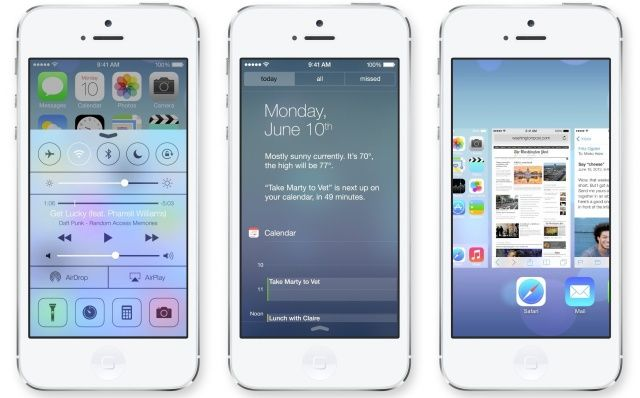
\includegraphics[width=10cm]{ios7.jpg}
	\caption{Nový vzhled iOS verze 7 \cite{ios-7-design}}
\end{figure}

S~dalším rokem a novým modelem iPhone 6 přišla verze iOS 8. iPhone 6 opět zásadně změnil svůj vzhled, ale v~operačním systému se moc zásadních změn nedělo. Apple se v~této verzi soustředil hlavně na nové funkce. Mezi ně se řadí \emph{Apple Music}, placení přes \emph{Apple Pay}, cloudové úložiště \emph{iCloud Drive}, sdílení práce mezi Apple zařízeními přes \emph{Handoff}, rodinné sdílení a další.

Rok 2015 přinesl iPhone 6S a iOS 9. V~této verzi se Apple soustředil hlavně na optimalizaci a stabilitu, příliš nových funkcí představeno nebylo – pouze nasvícení pro noční používání \emph{Night shift}, režim nízké spotřeby a možnost používat veřejný testovací beta program.

Dalším modelem byl v~roce 2016 iPhone 7 s~iOS~10. Opět nepřinesl moc nových funkcí, mimo například možnosti mazat původní nainstalované aplikace.

O~rok později poté s iPhonem~8 přišel iOS~11. V~této verzi se Apple soustředil převážně na nové funkcionality pro iPad, které se jeho použití snažily přiblížit k~plnohodnotnému počítači. Nově přibyly funkce jako podpora tužky \emph{Apple Pencil}, podpora více otevřených oken a pracovních ploch nebo prohlížeč souborů. Apple ale na závěr představení představil ještě další nový iPhone – iPhone X. Jednalo se o~další velký redesign, kdy se výrazně zvětšila plocha displeje, zmizelo přední tlačítko a vzniklo ověření uživatele pomocí obličeje – \emph{Face ID}.

V~roce 2018 Apple představil iPhone~XS a levnější variantu XR, se kterými přišel iOS~12, kde se jednalo opět jen o~mírná vylepšení. 

S~dalším rokem přišel iPhone~11 a iOS~13. Tento systém už se rozdělil – pro zařízení iPad nyní vznikl oddělený \emph{iPadOS}. V~iOS~13 Apple představil možnost tmavého režimu pro celý systém, nové možnosti bezpečnosti a soukromí a s~tím související možnost přihlášení přes Apple.

V~roce 2020 s~iPhonem~12 a iOS~14 Apple přidal několik menších změn a vylepšení, jako \emph{Widgety} na domovské obrazovce.

Podobně to bylo i~v~roce 2021, kdy Apple s~novým iPhonem~13 a iOS~15 přidával velké množství menších vylepšení, primárně do vlastních aplikací.

S~rokem 2022 přišel iPhone~14 a iOS~16, který přinesl sadu vylepšení a nových funkcí pro zamčenou obrazovku, spolu s~dalšími vylepšeními,

Poslední velký update iOS přišel v~roce 2023 s~iPhonem~15 a iOS~17. A jak už bylo v~posledních letech zvykem, tak tato aktualizace přinášela větší množství menších vylepšení a aktualizací, které ale už nijak zásadně neměnily systém a interakci s~ním. \cite{history-of-ios}

Za těchto 17 let vývoje se operační systém iOS dostal do stavu, kdy ho v~současnou chvíli používá 1,46 miliard aktivních uživatelů. Mobilních telefonů iPhone se od roku 2007 prodalo 2,3 miliard. \cite{iphone-user-statistics}

%---------------------------------------------------------------
\subsection{Vývojové nástroje a prostředí}\label{ios-dev-tools}
%---------------------------------------------------------------

Jak již bylo zmíněno v~předchozí sekci, obchod s~aplikacemi \emph{App Store} byl uživatelům dostupný od roku 2008. Ve stejnou dobu také Apple zpřístupnil vývojářům iPhone SDK ve svém vývojovém prostředí \emph{Xcode}. Toto vývojové prostředí od Applu již existovalo od roku 2003, kdy vzniklo jako rebranding původního vývojového prostředí \emph{Project Builder}. S~příchodem App Storu Apple umožnil všem vývojářům v~Xcodu vyvíjet aplikace pro iPhone OS od verze 2.0 pomocí zmíněného iPhone SDK. 

Vývojové prostředí Xcode je jednotné integrované vývojové prostředí, které slouží pro vývoj aplikací pro všechny platformy společnosti Apple. Lze stáhnout zdarma z~obchodu \emph{Mac App Store} nebo ze stránek společnosti Apple. Instalace vývojového prostředí obsahuje i~instalaci dalších pomocných nástrojů, jako je simulátor zařízení (iPhone, iPad, \dots), nástroje příkazové řádky, a další. \cite{xcode-history}

Pro nativní vývoj iOS aplikací se dříve používal programovací jazyk \emph{Objective-C} \cite{objc} a pro tvorbu uživatelského rozhraní knihovna \emph{UIKit}. V~roce 2014 Apple přidal podporu svého nového programovacího jazyku \emph{Swift} \cite{swift} a v~roce 2019 přidal podporu nové deklarativní knihovny pro tvorbu uživatelského rozhraní \emph{SwiftUI} \cite{swiftui}.

%---------------------------------------------------------------
\subsection{Architektura aplikací}\label{app-architecture}
%---------------------------------------------------------------

Jako u~každého softwarového projektu, architektura je důležitou součástí jeho návrhu. K~architekturám mobilních aplikací existuje mnoho přístupů. Například u~Android aplikací sám Google doporučuje, jaké architektonické vzory by měly být používány a doporučuje architektury pro tyto aplikace \cite{android-app-arch}. Apple přímo žádné architektury pro aplikace cílící na iOS platformu nedoporučuje. 

Dokumentace pro iOS platformu ale obsahuje mnoho ukázek kódu věnujících se konkrétním tématům (například \cite{swift-ui-tutorial-complex-interfaces}), kde je vždy nějaký náznak architektury připraven. V~těchto ukázkách se vyskytuje architektura \emph{Model-View-Controller} (zkráceně MVC). Narozdíl od tradiční MVC architektury se ta používaná Applem mírně liší, jelikož tradiční MVC architektura není moc dobře aplikovatelná na moderní iOS vývoj. Jak lze vidět na obrázcích \ref{fig:mvc}, v~tradičním MVC by mělo \emph{View} být beze stavu a měl by ho pouze překreslovat \emph{View Controller}. Toto sice je možné v~iOS aplikaci implementovat, ale nedává to moc smysl, protože všechny tyto 3 entity jsou hluboce provázané, což dramaticky snižuje jejich opětovné použití. Při použití v~iOS aplikaci je \emph{Controller} mediátorem mezi \emph{View} a \emph{Model}, kteří o~sobě navzájem nic nevědí. Jelikož je ale \emph{View Controller} zpravidla velice provázán s~\emph{View}, tak vzniká potřeba psát masivní \emph{View Controller}. Proto se v~iOS vývoji často referuje na MVC jako na \emph{Massive View Controller}.

\begin{figure}[h]
	\centering
	\begin{subfigure}[b]{0.35\textwidth}
		\centering
		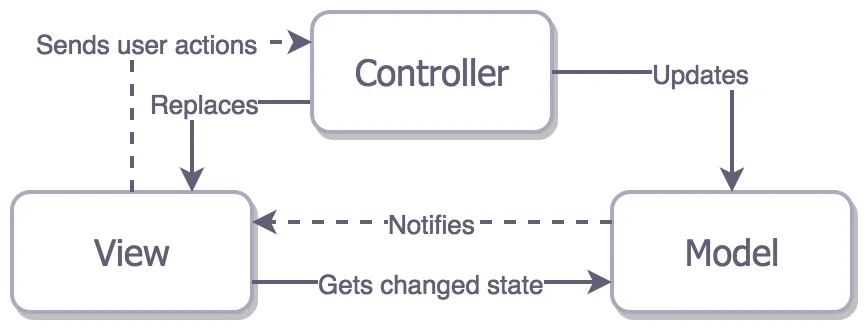
\includegraphics[width=6cm]{traditional-mvc.png}
		\caption{Tradiční MVC architektura}
	\end{subfigure}
	\hspace{1cm}
	\begin{subfigure}[b]{0.45\textwidth}
		\centering
		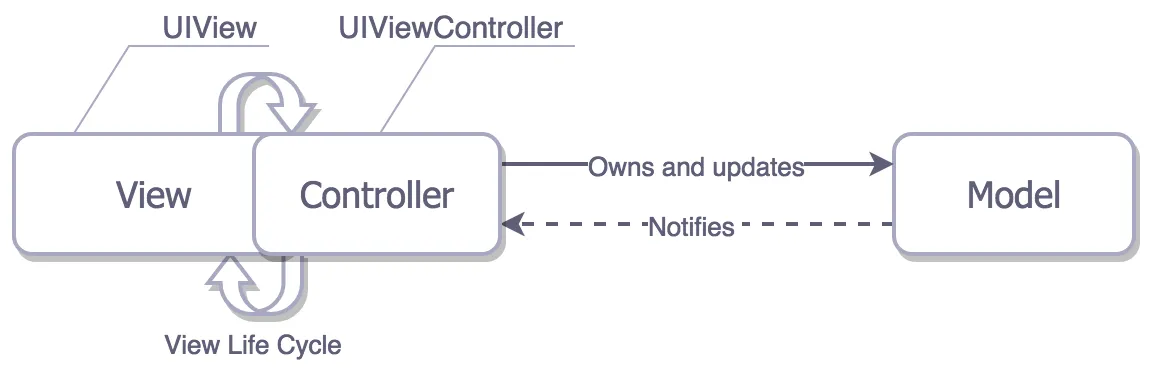
\includegraphics[width=7cm]{apple-mvc.png}
		\caption{MVC architektura v~iOS aplikacích}
	\end{subfigure}
	\caption{Architektura Model-View-Controller \cite{ios-architecture-patterns}}
	\label{fig:mvc}
\end{figure}

Architektura MVC je ale v~ukázkách kódu od Applu používána pravděpodobně převážně proto, protože se hodí pro výstižné a krátké ukázky kódu – obsahuje totiž minimální \emph{overhead}. Pro potřeby větších projektů začíná být nedostačující. Nelze nijak testovat logika prezentování, a \emph{View} také nelze pomocí jednotkových testů otestovat. Jediné, co lze testovat, je \emph{Model}. A velkou nevýhodou je právě zmíněný masivní \emph{View Controller}, který pro složitější obrazovky přestává být přehledný.

Velmi rozšířenou architekturou v~iOS vývoji je \emph{Model-View-ViewModel} (zkráceně MVVM). \emph{View} a \emph{Model} zastávají stejnou funkci jako v~MVC, a mediátorem je zde \emph{View Model}. \emph{View} je v~tomto případě konkrétní obrazovka a/nebo \emph{View Controller}. \emph{View Model} je nezávislý na knihovně uživatelského rozhraní, což umožňuje jeho lepší testovatelnost. Drží stav obrazovky, vyvolává změny pro \emph{Model} a aktualizuje se podle něj. Vizuální reprezentace architektury MVVM lze nahlédnout v~obrázku \ref{fig:mvvm}.

\begin{figure}[h]
	\centering
	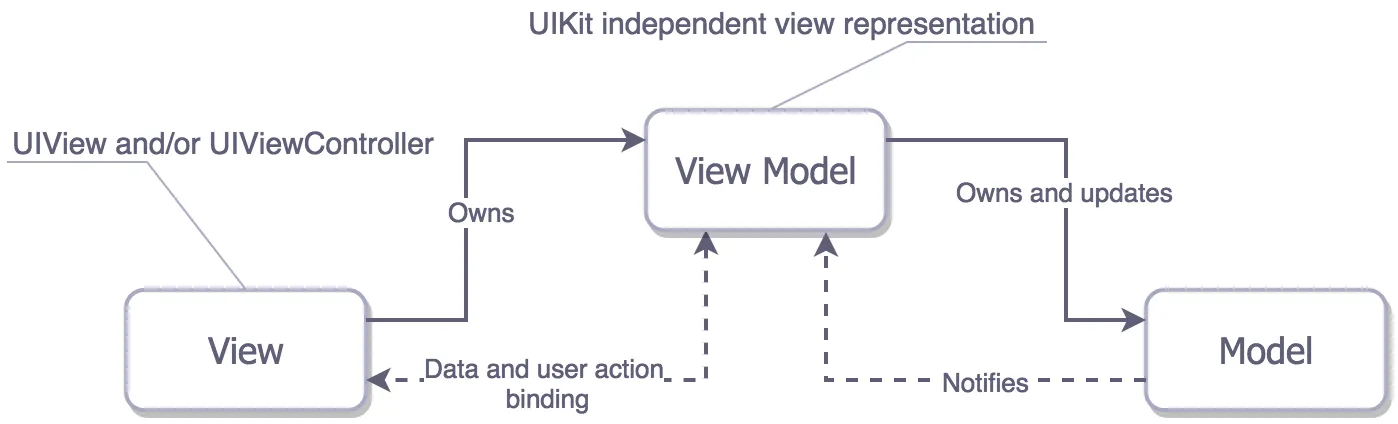
\includegraphics[width=10cm]{mvvm.png}
	\caption{Architektura MVVM \cite{ios-architecture-patterns}}
	\label{fig:mvvm}
\end{figure}

Další rozšířenou architekturou v~iOS aplikacích je \emph{Viper}. Tato architektura nepochází ze skupiny MV(X). \emph{Viper} se snaží vzít rozdělovaní odpovědností o~krok dále – obsahuje 5 vrstev:
\begin{itemize}
\item\textbf{View:} Zastává stejnou funkcionalitu jako v MV(X), tedy \emph{View} a/nebo \emph{View Controller}.
\item\textbf{Interactor:} Obsahuje byznysovou logiku související s~daty, jako tvorba instancí nebo načítání dat ze serveru.
\item\textbf{Presenter:} Obsahuje byznysovou logiku UI, ale je nezávislý na UI knihovně. Volá metody \emph{Interactoru}.
\item\textbf{Entities:} Čisté objekty dat.
\item\textbf{Router:} Odpovědný za přechody mezi \emph{Viper} moduly.
\end{itemize}
Tato architektura je poměrně volná v~tom, co bude konkrétní \emph{Viper} modul reprezentovat. Může to být jedna samotná obrazovka, ale může to být celá část aplikace. Lze si všimnout několika rozdílů od architektur ze skupiny MV(X):
\begin{itemize}
\item Model (interakce s~daty) je přesunut do \emph{Interactoru} pomocí \emph{Entities}.
\item Pouze povinnosti UI reprezentace \emph{Controlleru}/\emph{View Modelu} je přesunuta do \emph{Presenteru}, ale ne byznysová logika s~daty.
\item \emph{Viper} explicitně adresuje odpovědnost navigace, kterou řeší \emph{Router}.
\end{itemize}
Vizualizace architektury \emph{Viper} lze nahlédnout v~obrázku \ref{fig:viper}. \cite{ios-architecture-patterns}

\begin{figure}[h]
	\centering
	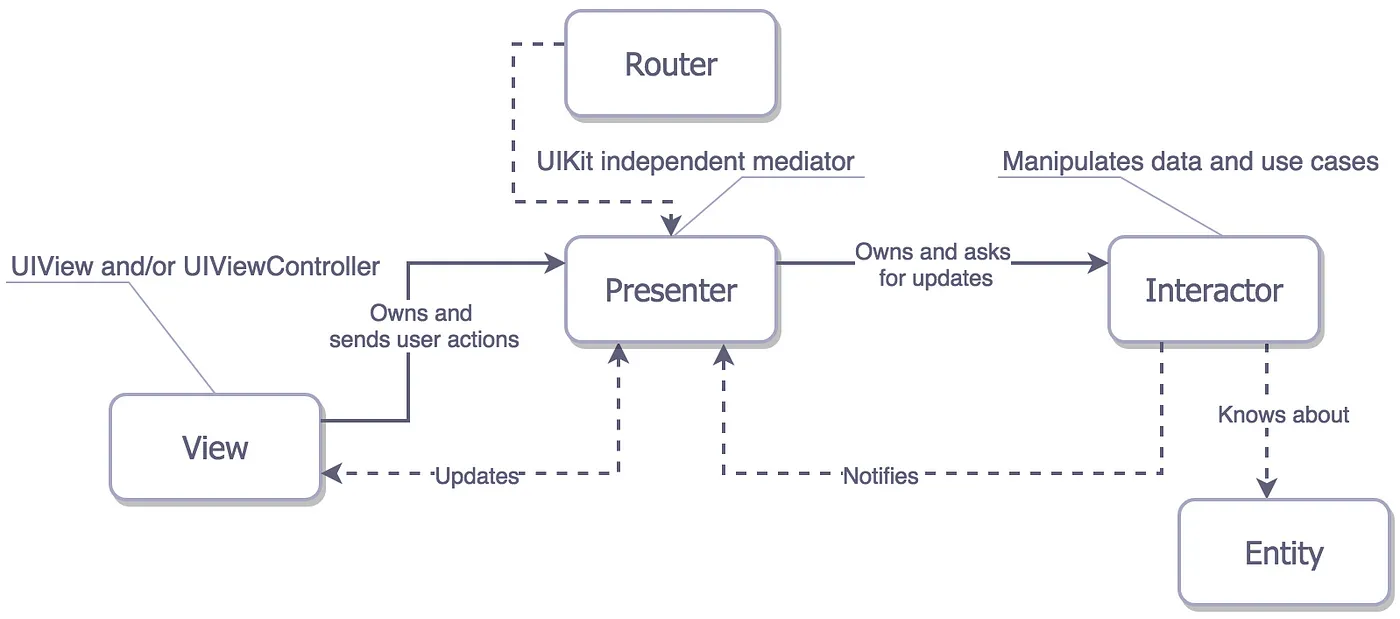
\includegraphics[width=12cm]{viper.png}
	\caption{Architektura \emph{Viper} \cite{ios-architecture-patterns}}
	\label{fig:viper}
\end{figure}

Existuje také rozšíření architektury MVVM o~navigační logiku, takzvaná MVVM-C, kde písmeno C představuje \emph{Flow Coordinator}. Tato vrstva je odpovědná za navigační tok, vytváří instance \emph{View} a/nebo \emph{View Controller} a prezentuje je, předává data mezi těmito instancemi a obsluhuje akce uživatele. Struktura \emph{Flow Coordinatoru} je vhodně navržena tak, aby se dala také dobře testovat. \cite{ios-mvvm-c}

Jednotlivé architektury mají také své aktualizované varianty pro nově používanou deklarativní UI knihovnu \emph{SwiftUI}. Všechny ze zmíněných architektur se dají vhodně použít i~s~touto knihovnou. Ve \emph{SwiftUI} už se jednotlivé obrazovky nerozdělují na \emph{View} a \emph{View Controller}, ale zůstává zde pouze \emph{View}. \emph{SwiftUI} ale ze své podstaty jako deklarativní knihovna přináší nové možnosti, jak k~architektuře aplikace přistupovat.

Jednou z~novějších architektur, které využívají výhody deklarativních UI knihoven, jako je \emph{SwiftUI}, je \emph{Model-View-Intent} (zkráceně MVI). \emph{View} a \emph{Model} reprezentují stejné vrstvy jako doposud a \emph{Intent} reprezentuje nějaký úmysl vyvolat určitou akci. Tím může být například kliknutí uživatele. Konkrétní \emph{Intent} poté pomocí nějaké byznysové logiky aktualizuje stav, podle kterého se následně aktualizuje \emph{View}. \cite{swiftui-mvi}

Všechny výše popsané architektury pracují s~daty pomocí nějakého \emph{Modelu} (\emph{Viper} pomocí \emph{Interactoru}). Práce s~daty ale obvykle není jednoduchá logika, která by si zasloužila pouze zmínku o~tom, že se o~ní stará nějaký \emph{Model}. Může se totiž jednat o~poměrně komplikovanou doménovou a byznysovou logiku, stahování dat ze serveru, cache dat, práce s~databází, a další. V~tomto ohledu je namístě diskutovat o~nějaké obecnější architektuře aplikace, ne pouze o~prezentační logice, tedy primárně o~logice uživatelského rozhraní. Obecným zvykem je aplikace rozdělovat do třívrstvé architektury. Tyto vrstvy se mohou nazývat různě, ale obvykle jde o:
\begin{itemize}
\item\textbf{Prezentační vrstva:} Logika uživatelského rozhraní, interakce s~uživatelem, obrazovky, \dots
\item\textbf{Doménová/byznysová vrstva:} Byznysová a doménová logika.
\item\textbf{Datová vrstva:} Práce s~daty (komunikace se serverem, databáze, \dots)
\end{itemize}
Rozšířená architektura, vhodná pro iOS aplikace, která definuje strukturu aplikace, je \emph{Clean Architecture}. Tato architektura je navržena pro dobrou testovatelnost, rozdělení odpovědnosti, a vyhovění dalším zašlým návrhovým vzorům týkajících se návrhu softwaru. V~této architektuře se jednotlivé vrstvy skládají z~následujících částí:
\begin{itemize}
\item\textbf{Prezentační vrstva:} \emph{View}, \emph{View Controllery}, \emph{View Modely}, a další, podle dané architektury (MVC, MVVM, Viper, \dots). Tato vrstva má závislost na doménové vrstvě a volá její \emph{Use Cases}.
\item\textbf{Doménová vrstva:} Rozhraní \emph{Use Cases} a jejich implementace, rozhraní \emph{Repositories}, které \emph{Use Cases} používají a doménové objekty. \emph{Use Cases} obsahují byznysovou logiku aplikace a datovou logiku nechávají na \emph{Repositories}.
\item\textbf{Datová vrstva:} Implementace \emph{Repositories}, rozhraní \emph{Providers} a implementace \emph{Providers}. Implementace repozitářů jsou nezávislé na konkrétních knihovnách třetích stran, obsahují logiku s~daty. Implementace \emph{Providers} už jsou závislé na konkrétních knihovnách. Jednotlivé \emph{Providers} se mohou starat například o~práci s~konkrétní databází nebo s~konkrétní knihovnou pro serverovou komunikaci.
\end{itemize}
V~\emph{Clean Architecture} se také pracuje s~\emph{Dependency Injection}, což řeší logiku toho, které konkrétní implementace budou dosazeny jednotlivým rozhraním (\emph{Use Cases, Repositories, Providers}). \cite{ios-clean-arch-mvvm}

%---------------------------------------------------------------
\section{Cross-platformní a multi-platformní možnosti}\label{crossplatform-multiplatform}
%---------------------------------------------------------------

V~současném prostředí mobilního vývoje se rozhodnutí ohledně vhodné platformy pro tvorbu aplikací stává klíčovým faktorem pro úspěch projektu. Existuje široká škála přístupů, které vývojáři mohou zvolit, od tradičních nativních řešení až po moderní multi-platformní a cross-platformní frameworky. Tato sekce se zaměřuje na analýzu těchto možností s~ohledem na tvorbu mobilní aplikace pro zaznamenávání odpracovaného času. Zhodnocuje jejich výhody, nevýhody a vhodnost pro konkrétní aplikaci. Tento přístup umožní lépe pochopit, jakým směrem se vydat při návrhu a implementaci projektu.

Pro rozdíl mezi cross-platformním a multi-platformním vývojem neexistuje přesná definice a v~různých zdrojích lze nalézt různé interpretace (např. \cite{cross-multiplatform-alternative-intepretation-one} a \cite{cross-multiplatform-alternative-intepretation-two}). V~kontextu vývoje pro mobilní aplikace si budeme tyto pojmy vykládat následovně:
\begin{itemize}
\item Cross-platformní vývoj představuje řešení, ve kterých sdílený kód běží na koncových platformách přímo přes nějakou formu abstrakce nebo interpretace.
\item Multi-platformní vývoj představuje řešení, ve kterých se sdílený kód přímo interpretuje do nativního kódu specifického pro každou platformu.
\end{itemize}

%---------------------------------------------------------------
\subsection{Nativní vývoj}
%---------------------------------------------------------------

Nativní vývoj pro platformu iOS znamená vytváření mobilních aplikací přímo v~jazyce \emph{Swift} nebo \emph{Objective-C} s~využitím oficiálních nástrojů poskytovaných společností Apple, jako je Xcode IDE a iOS SDK. Tento přístup umožňuje vytvořit aplikaci, která je optimalizovaná pro konkrétní operační systém a využívá všech funkcí a výhod, které iOS nabízí.

Výhody nativního vývoje pro iOS spočívají především v~plné integraci s~ekosystémem Apple, což zajišťuje vysokou kvalitu, rychlost a stabilitu aplikací. Vývojáři mají přístup ke kompletní sadě nástrojů, dokumentace a podpory přímo od výrobce platformy, což usnadňuje vývoj a řešení potíží. Díky nativnímu přístupu je možné vytvářet aplikace s~vysokou výkonností a možnostmi, které jsou na míru prostředí iOS.

Nevýhody nativního vývoje spočívají v~tom, že vyžaduje znalost specifických jazyků a nástrojů pro každou platformu (\emph{Swift}/\emph{Objective-C} pro iOS, \emph{Kotlin}/\emph{Java} pro Android), což může zvýšit náklady na vývoj a časovou náročnost. Navíc nativní přístup vyžaduje oddělený vývoj pro každou platformu, což může být neefektivní pro projekty s omezeným rozpočtem nebo krátkým časovým rámcem.

Nativní vývoj je ideální pro projekty, které se zaměřují na plné využití možností iOS platformy, jako jsou výkonné aplikace nebo aplikace s~náročnějším uživatelským rozhraním. Také je vhodný pro aplikace, které potřebují maximální stabilitu a bezpečnost, například bankovní aplikace nebo aplikace pro zpracování citlivých údajů. Pro vývojáře, kteří chtějí mít plnou kontrolu nad každým aspektem aplikace a využít všech funkcí, které iOS nabízí, je nativní vývoj nejlepší volbou.

%---------------------------------------------------------------
\subsection{Cross-platformní vývoj}
%---------------------------------------------------------------

Cross-platformní vývoj se zaměřuje na tvorbu mobilních aplikací, které mohou běžet na více než jedné platformě (např. iOS a Android) s~využitím jediného kódu a jednoho vývojového prostředí. Tento přístup umožňuje vývojářům sdílet co nejvíce kódu mezi různými platformami, čímž snižuje náklady a zjednodušuje správu aplikací pro různé zařízení.

Mezi hlavní výhody cross-platformního vývoje patří efektivita a rychlost vývoje díky sdílení kódu mezi platformami. Vývojáři mohou využít frameworky jako \emph{Flutter} \cite{flutter-cross-platform}, \emph{React Native} \cite{react-native-cross-platform} nebo \emph{Xamarin} \cite{xamarin-cross-platform}, které umožňují psát kód v~populárních jazycích (např. \emph{JavaScript}, \emph{TypeScript}, \emph{Dart}, \emph{C\#}) a následně ho spouštět na různých platformách. Tento přístup také usnadňuje aktualizace a údržbu aplikací, protože změny se projeví na všech podporovaných platformách současně.

Nevýhody cross-platformního vývoje se mohou projevit ve snížené flexibilitě a omezení přístupu k~některým pokročilým funkcím a knihovnám specifickým pro danou platformu. Rovněž může docházet k~omezení rychlosti nebo výkonu aplikace v~porovnání s~nativními aplikacemi. Další nevýhodou může být závislost na externích frameworcích a jejich aktualizacích.

Cross-platformní vývoj je ideální pro projekty, které vyžadují rychlou dostupnost na více platformách s~omezenými zdroji. Hodí se pro aplikace s~jednodušším uživatelským rozhraním, obsahově orientované aplikace (např. novinky, e-commerce), nebo pro firemní aplikace, které nevyžadují specifické funkce jednotlivých platforem. Tento přístup je také vhodný pro malé a střední projekty, kde je důležitá rychlá a efektivní tvorba aplikace pro více platforem.

%---------------------------------------------------------------
\subsection{Multi-platformní vývoj}
%---------------------------------------------------------------

Multi-platformní vývoj se liší od cross-platformního vývoje tím, že přímo kompiluje zdrojový kód do nativního kódu specifického pro každou platformu, místo aby spoléhal na vrstvu abstrakce nebo interpretaci. To znamená, že výsledná aplikace běží jako nativní aplikace bez vrstvy prostřednictvím frameworku. Typickým příkladem multi-platformního vývoje je použití jazyka jako \emph{Kotlin} pro Android a \emph{Kotlin/Native} pro iOS, které se kompilují do nativního kódu pro obě platformy. Tato technologie se nazývá \emph{Kotlin Multiplatform} \cite{kotlin-multiplatform}.

Výhody multi-platformního vývoje zahrnují možnost sdílet větší část kódu mezi různými platformami a zároveň dosahovat výkonnosti a funkčnosti nativních aplikací. To znamená, že vývojáři mohou využívat specifické funkce a knihovny pro každou platformu, aniž by se museli spoléhat na obecné abstraktní vrstvy. Tento přístup také umožňuje lepší optimalizaci výkonu a přístup k pokročilým funkcím operačních systémů.

Nevýhody multi-platformního vývoje mohou zahrnovat větší složitost a náročnost vývoje oproti čistě cross-platformním frameworkům. Každá platforma může vyžadovat jiné postupy a úpravy, ačkoli základní kód je sdílen. Některé specifické funkce nebo optimalizace pro konkrétní platformu mohou být obtížnější dosáhnout pomocí multi-platformního přístupu než s nativním vývojem.

Multi-platformní vývoj je vhodný pro projekty, které vyžadují vysokou výkonnost a přístup k nativním funkcím a knihovnám, ale zároveň potřebují sdílet co nejvíce kódu mezi platformami. Ideální je pro rozsáhlejší projekty nebo aplikace, které potřebují plnou integraci s operačním systémem, ale zároveň chtějí minimalizovat duplicitu práce a zjednodušit správu a údržbu kódu. Multi-platformní vývoj je také vhodný pro situace, kdy je důležitá konzistence a shoda funkcí mezi různými verzemi aplikace na různých platformách.

%---------------------------------------------------------------
\section{Backendová řešení pro mobilní aplikace}\label{backend}
%---------------------------------------------------------------

Backendová část mobilních aplikací hraje klíčovou roli v~poskytování dat, zpracování požadavků a správě uživatelských účtů a obsahu. Tato sekce se zaměřuje na analýzu různých backendových řešení a technologií, které jsou vhodné pro podporu mobilních aplikací. Při výběru správného backendového řešení je důležité pochopit úlohu, kterou backend hraje v~kontextu mobilního prostředí a identifikovat faktory, které ovlivňují výběr a implementaci.

Backendová část mobilní aplikace zajišťuje komunikaci mezi klientem (mobilní aplikací) a serverem, zpracování dat, autentizaci uživatelů, a další potřebné funkce. Tento centrální prvek infrastruktury zabezpečuje efektivní a spolehlivé fungování mobilních aplikací, přičemž umožňuje sdílení dat mezi různými zařízeními a poskytuje uživatelům personalizovaný a interaktivní zážitek.

Při výběru backendového řešení pro mobilní aplikaci je důležité zvážit několik faktorů. Patří mezi ně škálovatelnost a výkon serveru, podpora pro bezpečnostní standardy a autentizaci, možnosti správy uživatelských dat, a také kompatibilita s~konkrétními požadavky a technologiemi použitými ve frontendové části aplikace. Dále je důležité zvážit náklady na provoz, údržbu a rozvoj backendového systému v průběhu životního cyklu aplikace.

Existuje široká škála backendových technologií a frameworků, které lze použít při vývoji mobilních aplikací. Od tradičních serverových platforem a frameworků až po moderní cloudová řešení a služby. Každá možnost má své vlastní výhody a nevýhody. Důkladná analýza těchto možností je zásadní k~správnému výběru backendové architektury pro konkrétní mobilní aplikaci.

%---------------------------------------------------------------
\subsection{Backend as a Service (BaaS) a jiná delegovaná řešení}\label{baas}
%---------------------------------------------------------------

Tato podsekce se zaměřuje na možnosti, kdy jsou části backendové infrastruktury mobilní aplikace outsourcovány na externí poskytovatele služeb, jako je \emph{Firebase}, \emph{AWS Amplify} nebo \emph{Parse}. Tento přístup umožňuje vývojářům rychle nasadit backendovou část aplikace bez nutnosti spravovat a udržovat vlastní serverovou infrastrukturu.

Jednou z~hlavních výhod BaaS je urychlení vývoje aplikace a snížení nákladů a komplexity provozování backendu. Poskytovatelé BaaS nabízejí hotová řešení pro autentizaci uživatelů, ukládání dat, notifikace, analýzu chování uživatelů a řadu dalších funkcí, což umožňuje vývojářům zaměřit se více na samotnou funkcionalitu aplikace a méně na infrastrukturální detaily.

Další výhodou je škálovatelnost a výkon poskytovaných služeb, který může být optimalizován poskytovatelem a automaticky přizpůsobován podle potřeb aplikace. Tento přístup je obzvláště užitečný pro malé a střední projekty s~omezenými zdroji nebo pro projekty, které potřebují rychle nasadit MVP (Minimum Viable Product) bez investice do vlastní infrastruktury.

Nevýhodou použití BaaS může být omezení v~možnostech škálování a přizpůsobení, zejména u složitějších aplikací nebo projektů se specifickými požadavky na infrastrukturu. Dále může být problémem závislost na externím poskytovateli služeb a jejich možná změna podmínek nebo dostupnosti.

Jako příklad BaaS lze uvést \emph{Firebase} od společnosti Google \cite{firebase}. Firebase poskytuje širokou škálu služeb, včetně realtime databáze, autentizace, cloudového úložiště, notifikací, analýzy a mnoha dalších. Tato platforma je oblíbená mezi vývojáři pro svou jednoduchost a širokou nabídku poskytovaných funkcí, což umožňuje rychlý vývoj a nasazení mobilních aplikací s~minimálním úsilím na správu backendové infrastruktury.

Dalšími příklady BaaS služeb jsou \emph{AWS Amplify} od společnosti Amazon \cite{aws-amplify} a \emph{Parse} \cite{parse}, který je open-source frameworkem pro tvorbu aplikací. Tyto služby nabízejí podobné funkce jako \emph{Firebase} a umožňují vývojářům využít hotová řešení pro backendovou část svých mobilních aplikací bez nutnosti psát a spravovat vlastní kód pro serverovou stranu.

%---------------------------------------------------------------
\subsection{Vývoj vlastního backendu}
%---------------------------------------------------------------

Tato sekce se zaměřuje na možnosti vytvoření a implementace vlastního backendového řešení pro podporu mobilních aplikací. Tento přístup umožňuje vývojářům plnou kontrolu nad backendovou infrastrukturou a její přizpůsobení specifickým požadavkům aplikace.

Jednou z~hlavních výhod vývoje vlastního backendu je možnost plného přizpůsobení infrastruktury a funkcí podle konkrétních potřeb mobilní aplikace. Vývojáři mají kontrolu nad škálovatelností, bezpečností a výkonem backendu, což je zvláště důležité pro aplikace s~vyššími nároky na bezpečnost, správu dat nebo specifické obchodní požadavky.

Další výhodou je snížená závislost na externích poskytovatelích služeb a jejich změnách v~podmínkách či dostupnosti. Vlastní backend umožňuje také integraci s~existujícími systémy a infrastrukturou v~organizaci, což může být podstatné pro firemní aplikace nebo projekty s~komplexními integračními požadavky.

Nevýhodou vývoje vlastního backendu může být zvýšená náročnost a časová zátěž vývoje a údržby. Vývojáři si musí sami implementovat všechny potřebné funkce backendu, včetně autentizace, ukládání dat, správy uživatelů a dalších. To může vést ke zvýšeným nákladům a časovému zpoždění při nasazení aplikace na trh.

Mezi nejpoužívanější řešení pro vývoj vlastního backendu patří frameworky jako \emph{Node.js} \cite{node-js} s~frameworky \emph{Express} \cite{node-js-express} nebo \emph{NestJS} \cite{nest-js} pro \emph{JavaScript}/\emph{TypeScript}, \emph{Ruby on Rails} \cite{ruby-on-rails} pro \emph{Ruby}, \emph{Django} \cite{django} pro \emph{Python} nebo \emph{Spring Boot} \cite{spring-boot} pro \emph{Javu}. Tyto frameworky nabízejí komplexní sadu nástrojů pro rychlý vývoj a nasazení backendové aplikace s~podporou různých funkcí, včetně routování, databázového přístupu, autentizace a dalších.

Každý z~těchto frameworků má své výhody a nevýhody. Například \emph{Node.js} s~\emph{Express} je velmi populární pro svou rychlost a flexibilitu, zatímco \emph{Spring Boot} je oblíbený pro svou robustnost a škálovatelnost v~prostředí \emph{Java} \cite{spring-boot-vs-node-js}. Výběr správného frameworku závisí na preferencích vývojářů, technologických požadavcích a cílech aplikace.

%---------------------------------------------------------------
\subsection{Databáze}
%---------------------------------------------------------------

Implementace databáze je dalším důležitým prvkem vývoje vlastního backendu pro mobilní aplikace, neboť poskytuje úložiště pro data, která aplikace zpracovává a uchovává. Existuje několik možností pro implementaci databází v~rámci backendového prostředí, které se liší podle typu databáze a potřeb aplikace.

Mezi nejpoužívanější řešení patří relační databáze, jako je \emph{Oracle Database} \cite{oracle-database} nebo \emph{PostgreSQL} \cite{postgresql}, a také \emph{noSQL} databáze, jako je \emph{MongoDB} \cite{mongodb} nebo \emph{Redis} \cite{redis}. Relační databáze jsou založené na modelu relačního datového skladu s~použitím \emph{SQL} (Structured Query Language) pro manipulaci s~daty. Tyto databáze jsou vhodné pro aplikace, které vyžadují komplexní transakční operace a silné zajištění integrity dat. Na druhou stranu \emph{noSQL} databáze jsou navrženy tak, aby byly flexibilnější a lépe škálovatelné pro různé typy dat. Jsou ideální pro aplikace, které mají různorodá data a vyžadují rychlý a flexibilní přístup k~nim.

Výhody relačních databází zahrnují silnou konzistenci dat, vysokou integritu a možnost provádět komplexní dotazy pomocí SQL. Na druhou stranu \emph{noSQL} databáze nabízejí vyšší škálovatelnost, flexibilitu datového modelu a lepší výkon pro určité aplikace s~velkým objemem dat. \cite{fit-lecture-no-sql}

Výběr správného typu databáze závisí na specifických požadavcích a charakteristikách projektu. Pro aplikace s~potřebou silné konzistence a transakcí jsou vhodné relační databáze, zatímco pro aplikace s~velkým objemem různorodých dat a vyššími požadavky na škálovatelnost jsou vhodnější \emph{noSQL} databáze.

Výběr implementace databázového řešení lze také outsourcovat na externí poskytovatele služeb BaaS. Jak bylo zmíněno v~sekci \ref{baas}, poskytovatelé jako \emph{Firebase} \cite{firebase} nebo \emph{AWS Amplify} \cite{aws-amplify} již implementují databázové řešení, které lze v~rámci těchto platforem využít. Existují také řešení, která poskytují pouze databázi jako externí řešení. Tato řešení jsou někdy nazývána DBaaS (Database as a Service) \cite{mongodb-dbaas}. Příkladem tohoto řešení je například \emph{MongoDB Atlas} \cite{mongodb-atlas}, právě pro databázi \emph{MongoDB}.

V implementaci vlastního backendu pro mobilní aplikace je důležité pečlivě zvážit výběr databázového řešení, aby byly splněny požadavky na výkon, škálovatelnost a bezpečnost aplikace. Zvážení výhod a nevýhod jednotlivých databázových systémů pomůže zajistit optimální implementaci a správu dat pro mobilní aplikaci pro zaznamenávání odpracovaného času.

%---------------------------------------------------------------
\section{Závěr analýzy}
%---------------------------------------------------------------

V~této kapitole byly probrány všechny informace potřebné pro navazující návrh mobilní aplikace pro zaznamenávání odpracovaného času. 

Co se týče domény problému, tak byla provedena rešerše spouštěčů měření času, ze které mohou být vhodně navrženy požadavky pro aplikaci na propojení s~nimi. Dále byla také provedena rešerše existujících systémů pro zaznamenávání odpracovaného času, ze které lze také vhodným způsobem navrhnout požadavky na integraci s~těmito systémy.

Dále se kapitola věnovala vývoji mobilních aplikací pro systém iOS, různým možnostem cross-platformního a multi-platformního vývoje a možnostem, jak přistupovat k~backendovým řešením podporující mobilní aplikace. Tyto informace by měly být plně postačující pro vhodný návrh funkcionalit aplikace, jejího uživatelského rozhraní, vnitřní architektury a nástrojů k~tomu potřebným.













































%---------------------------------------------------------------
\chapter{Návrh}
%---------------------------------------------------------------

Tato kapitola se věnuje návrhu aplikace, tedy technologické architektury celé platformy a jednotlivých implementací, návrhu funkcionalit a uživatelskému rozhraní aplikace. V~následujících sekcích budou rozebírány jednotlivé navržené funkcionality a jejich rozhraní. Nejprve je ale potřeba si stanovit nějaký vzhledový styl aplikace.

Pro návrh uživatelského rozhraní aplikace byl použit nástroj \emph{Figma} \cite{figma}, dále byly použity zdroje z~šablony \emph{Apple Design Resources} \cite{apple-design-resources}.

%---------------------------------------------------------------
\section{Vzhledový styl aplikace}
%---------------------------------------------------------------

Aplikace cílí na platformu iOS, což bude důležitou součástí jejího návrhu. Apple definuje rozsáhlou příručku pro návrh uživatelského rozhraní pro platformu iOS \cite{apple-design-guidelines-ios} a návrh aplikace se touto příručkou bude v~mnoha ohledech řídit.

Každá aplikace má nějaký svůj vzhledový styl, který definuje základní barvy, které bude aplikace používat, vzhledy tlačítek, textových polí, fontů a dalšího. Následující definice těchto prvků vychází převážně z~osobní preference, která se soustředí spíše na jednoduchost a ne příliš velkou výraznost rozhraní. Cílem tedy bude se přiblížit systémovému vzhledu platformy iOS a přidat vlastní mírný vzhledový jazyk.

%---------------------------------------------------------------
\subsection{Barvy}
%---------------------------------------------------------------

Základní návrh barev aplikace lze nahlédnout v~obrázku \ref{fig:colors}. Barvy jsou navrženy tak, aby vždy vznikl dostatečný kontrast mezi barvou pozadí a barvou popředí.

\begin{figure}[h]
	\centering
	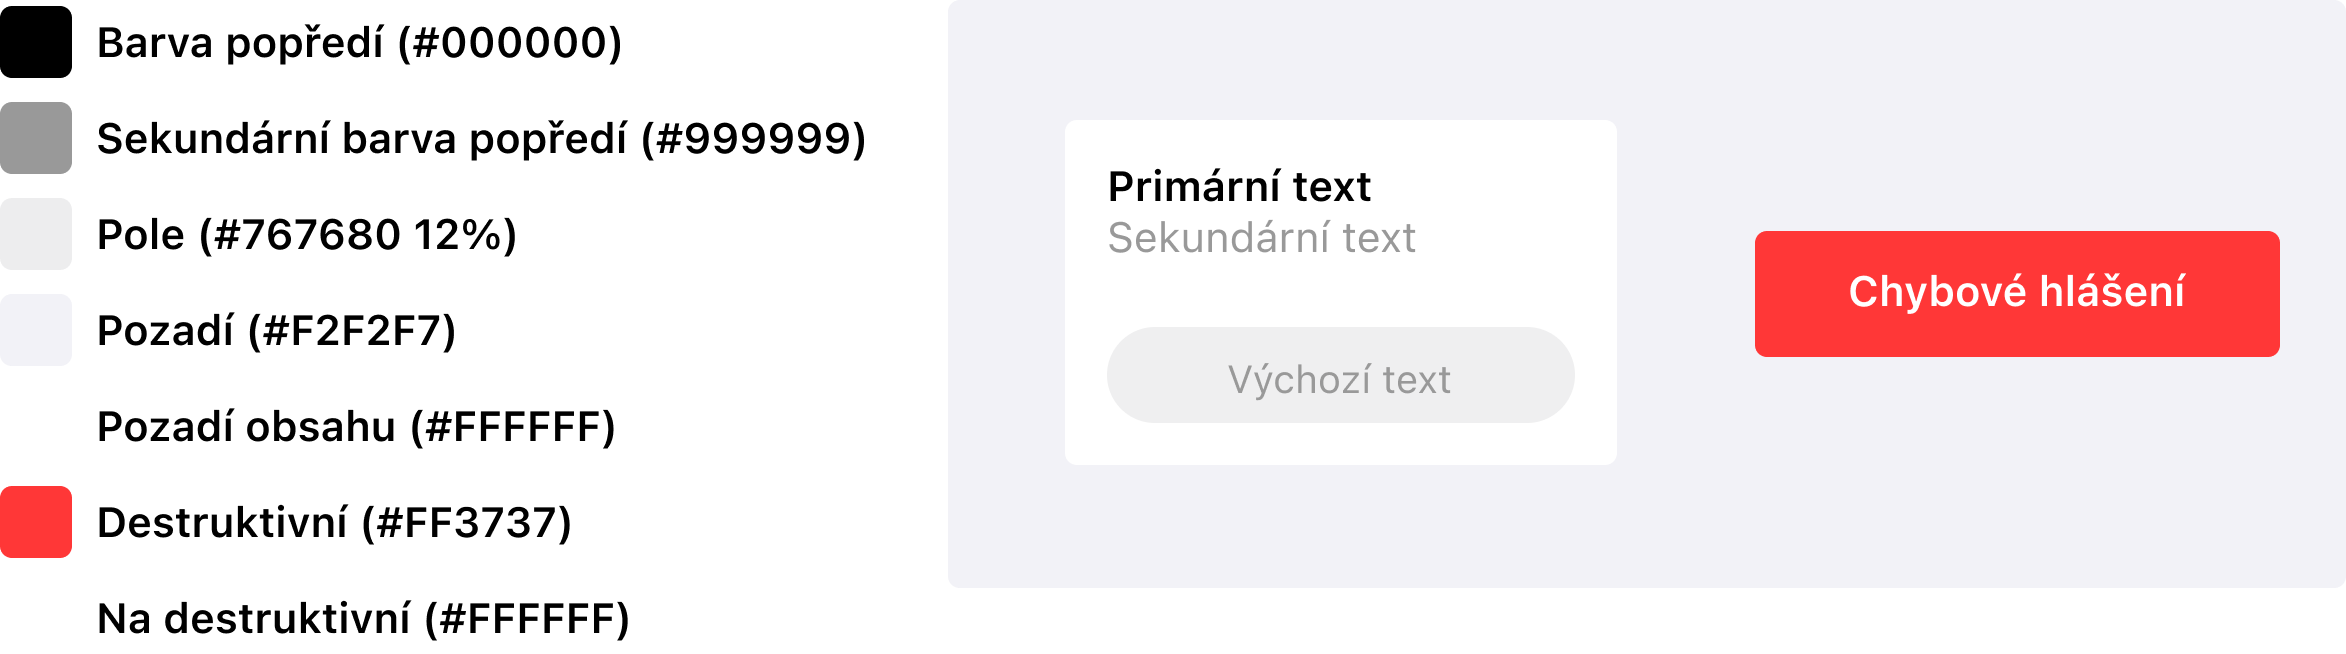
\includegraphics[width=\textwidth]{colors.png}
	\caption{Vzhledový styl aplikace – Barvy}
	\label{fig:colors}
\end{figure}

%---------------------------------------------------------------
\subsection{Fonty}
%---------------------------------------------------------------

Základní návrh fontů lze nahlédnout v~obrázku \ref{fig:fonts}. Daný font bude vždy používat systémovou rodinu fontů, tedy obvykle \emph{San Francisco} (SF). Jednotlivé velikosti jsou pouze referenční, protože aplikace by měla podporovat dynamické fonty a reflektovat tak škálování uživatele. Daná velikost je tedy velikost pro výchozí nastavení škálování textu.

\begin{figure}[h]
	\centering
	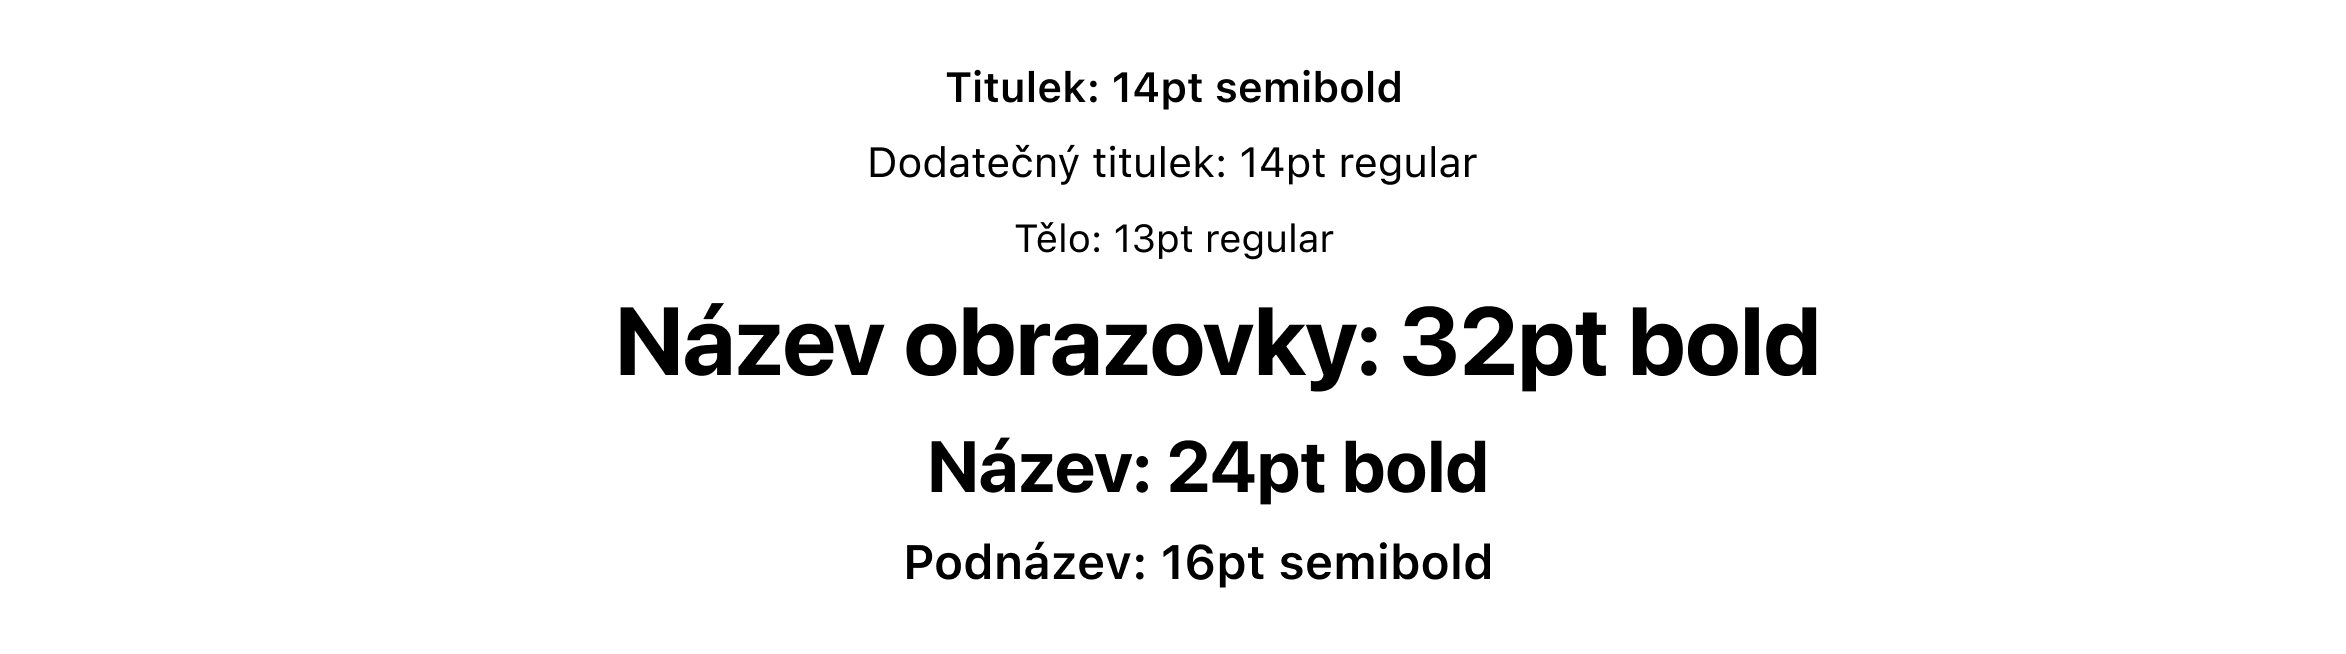
\includegraphics[width=\textwidth]{fonts.png}
	\caption{Vzhledový styl aplikace – Fonty}
	\label{fig:fonts}
\end{figure}

%---------------------------------------------------------------
\subsection{Prvky}
%---------------------------------------------------------------

Návrh prvků rozhraní vychází z~již definovaných barev a fontů, lze jej nahlédnout v~obrázku \ref{fig:elements}.

\begin{figure}[h]
	\centering
	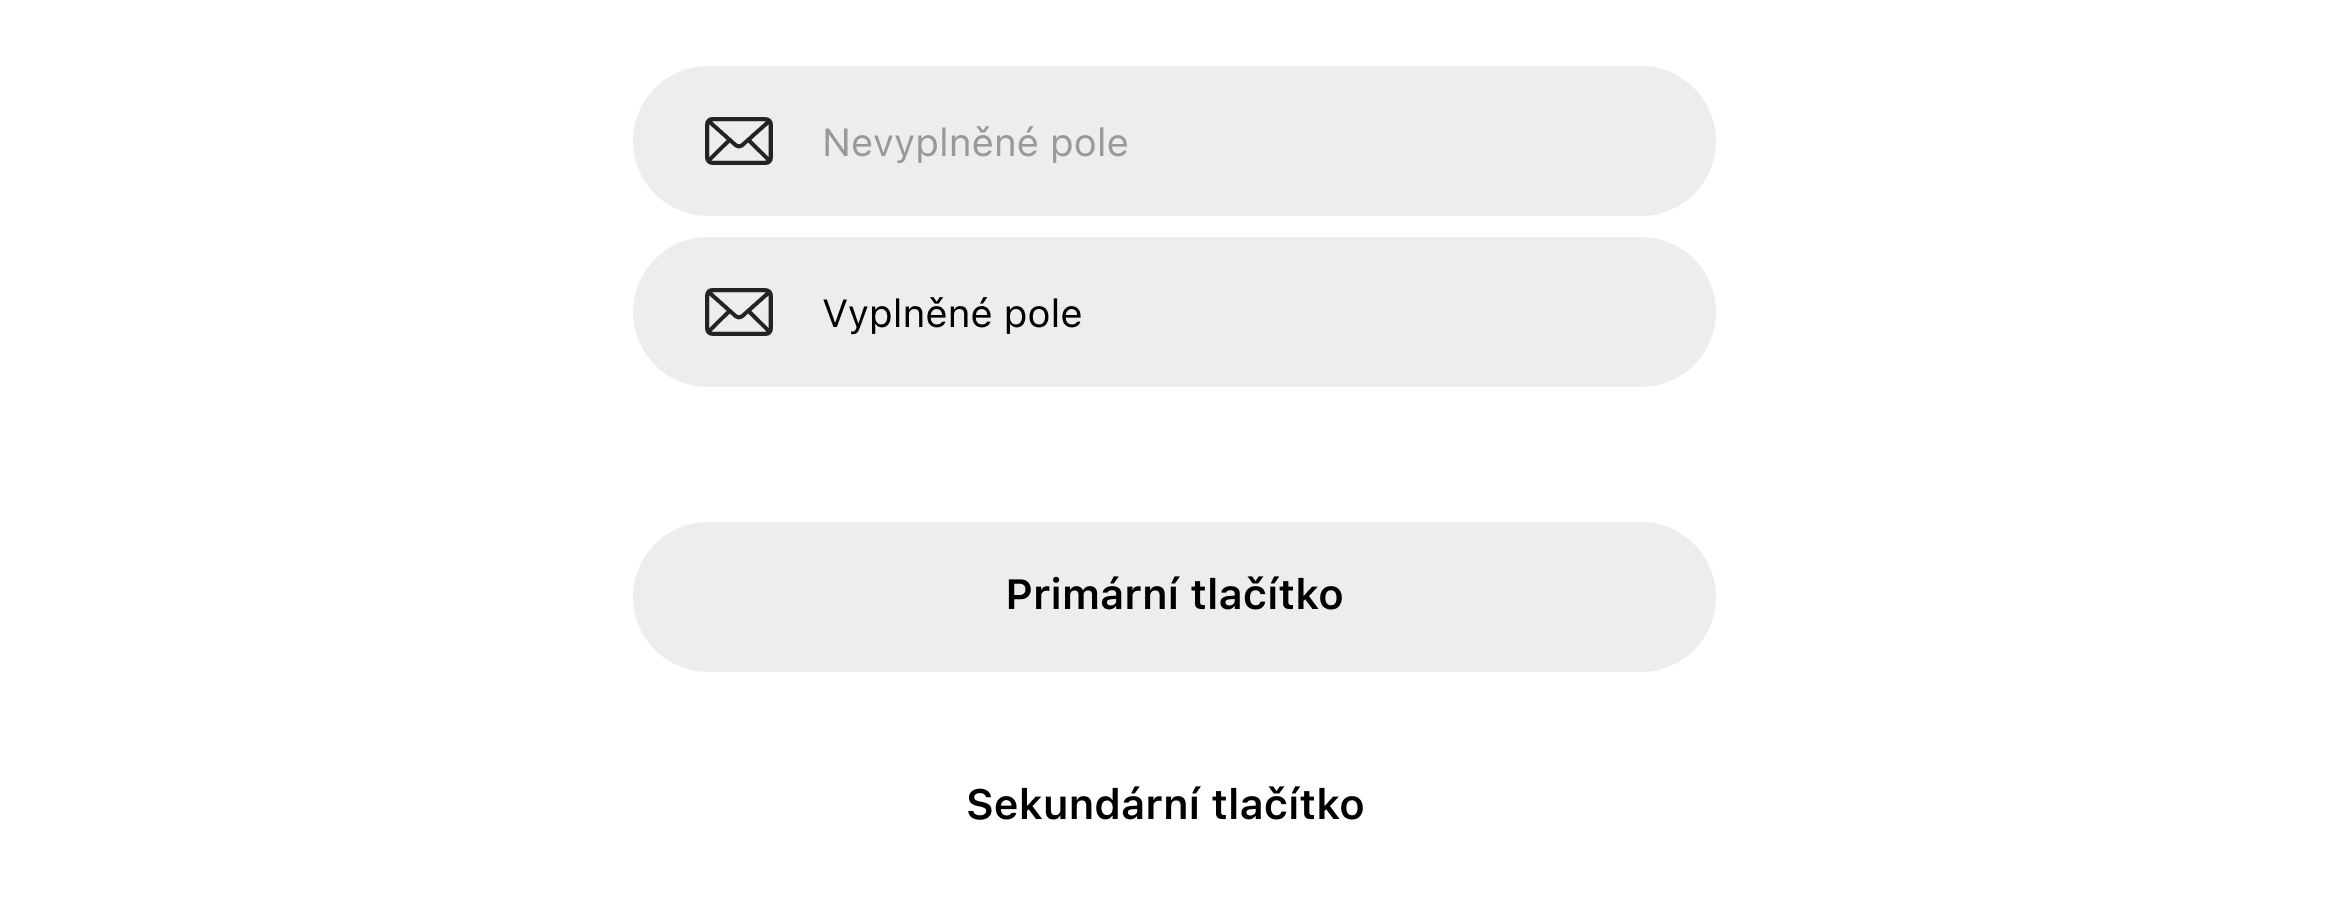
\includegraphics[width=\textwidth]{elements.png}
	\caption{Vzhledový styl aplikace – Prvky}
	\label{fig:elements}
\end{figure}

Na všechny ostatní prvky, jako prvky navigace, seznamy, alerty, a další, bude využito systémových prvků. Tím bude nejlépe vyhověno vzhledové příručce firmy Apple, pouze budou upravné některé barvy těchto prvků, aby ladily k~vzhledu aplikace.

%---------------------------------------------------------------
\subsection{Název a ikona}
%---------------------------------------------------------------

Návrh chytlavého názvu bývá obvykle složitá věc. Pro tuto aplikaci byl zvolen název \emph{Trackee} (anglicky [tra·ki]), který je odvozen z~anglického pojmu \emph{Time tracking}, což představuje měření odpracovaného času. Koncovka \emph{-ee} je také poslední dobou častou volbou pro názvy různorodých aplikací, jako \emph{Spendee} \cite{spendee}, \emph{Fondee} \cite{fondee} a další. Pod tímto názvem není registrována žádná ochranná známka \cite{upd-database}, ani není veden žádný záznam u~správce české domény \cite{cz-nic-trackee}.

Ikona aplikace také neprocházela nijak složitým procesem návrhu, byl pouze použit systémový symbol časovače na pozadí s~barvami aplikace popředí a pole. Ikonku lze nahlédnout v~obrázku \ref{fig:app-icon}.

\begin{figure}[h]
	\centering
	
\includegraphics[width=5cm]{trackee.png}
	\caption{Ikona aplikace}
	\label{fig:app-icon}
\end{figure}

%---------------------------------------------------------------
\section{Funkcionality aplikace a jejich uživatelské rozhraní}\label{features}
%---------------------------------------------------------------

Aplikace bude primárně sloužit pro zaznamenávání odpracovaného času. Je tedy potřeba, aby každý uživatel měl možnost si vytvářet vlastní záznamy a další data, která budou propojena pouze s~ním, a ke kterým bude mít přístup pouze on. Toto obvyklý případ užití mobilní aplikace, který ze své podstaty vyžaduje nějakou formu vytvoření uživatelského účtu, se kterým budou data propojena, a jeho autentizace. Nejobvyklejším způsobem autentizace je autentizace pomocí e-mailu a hesla. Tento způsob je i~poměrně jednoduchý z~hlediska implementace a spousta poskytovatelů BaaS (Backend as a Service, vizte \ref{baas}) tento způsob autentizace implementuje. 

%---------------------------------------------------------------
\subsection{Přihlášení a registrace}\label{feature-onboarding}
%---------------------------------------------------------------

Přihlašovací obrazovka bude obsahovat pouze nadpis, pole pro vyplnění e-mailu, hesla, primární tlačítko pro přihlášení a sekundární tlačítko pro registraci. Obrazovka pro registraci, která se otevře po kliku na tlačítko pro registraci, poté bude od uživatele potřebovat také jen e-mail a heslo, které je ale zvykem napsat dvakrát, aby se snížila šance, že se v~něm vyskytl překlep. Obrazovky přihlášení a registrace lze nahlédnout v~obrázku \ref{fig:onboarding}. Úspěšné přihlášení a registrace uživatele přesměruje na hlavní obrazovku aplikace.

\begin{figure}[h]
    \centering
    \begin{subfigure}[b]{0.4\textwidth}
		\centering
		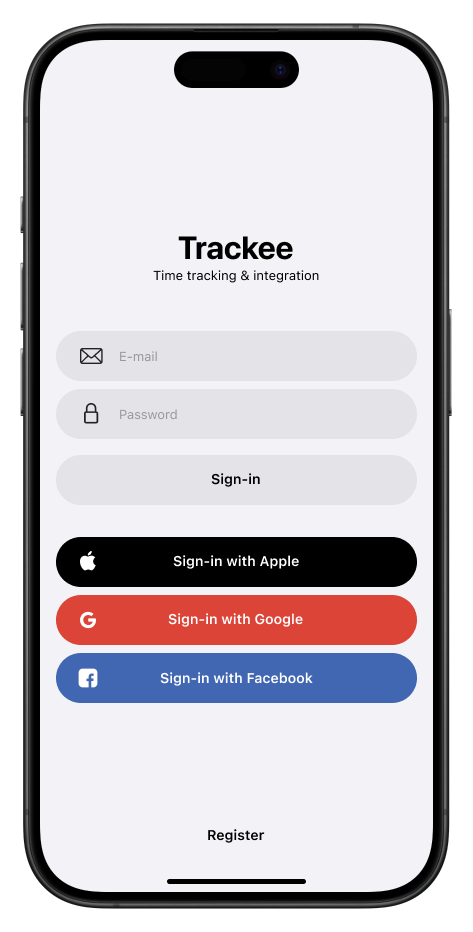
\includegraphics[width=6cm]{login.png}
		\caption{Přihlášení}
		\label{fig:login}
	\end{subfigure}
	\hspace{2cm}
	\begin{subfigure}[b]{0.4\textwidth}
		\centering
		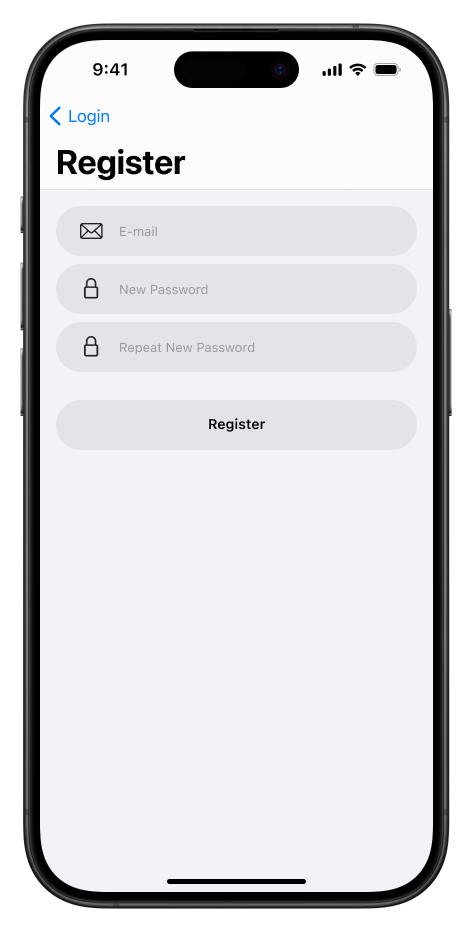
\includegraphics[width=6cm]{register.png}
		\caption{Registrace}
	\end{subfigure}
	\caption{Onboarding}
	\label{fig:onboarding}
\end{figure}

%---------------------------------------------------------------
\subsection{Lišta karet a časovač}\label{feature-timer}
%---------------------------------------------------------------

Navigace mezi hlavními obrazovkami aplikace bude řešena pomocí lišty karet, jelikož se jedná o~častý a doporučený způsob, jak navigovat mezi vzájemně exkluzivními částmi obsahu \cite{apple-guidelines-tabbars}. Hlavní obrazovkou bude přehled, na kterém bude uživatel moct ovládat časovač, a kde uvidí historii svých časových záznamů, seřazenou od nejnovějších po nejstarší. Jelikož pro uživatele je nejjednodušší dosáhnout na ovládací prvky, které jsou ve spodní části displeje, bude ovládání časovače umístěno ve spodní části obrazovky, a časové záznamy se budou řadit nad ním. Návrh této obrazovky lze nahlédnout na obrázku \ref{fig:timer}.

\begin{figure}[h]
    \centering
    \begin{subfigure}[b]{0.4\textwidth}
		\centering
		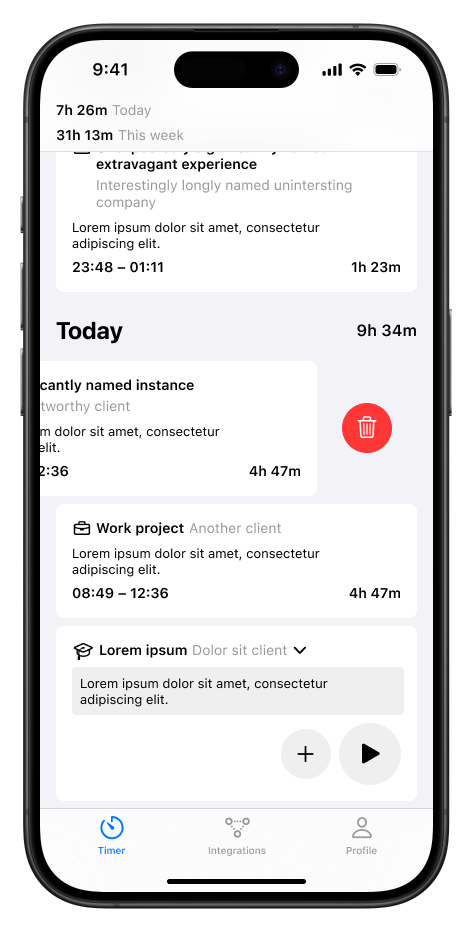
\includegraphics[width=6cm]{timer.png}
		\caption{Časovač}
		\label{fig:timer}
	\end{subfigure}
	\hspace{2cm}
	\begin{subfigure}[b]{0.4\textwidth}
		\centering
		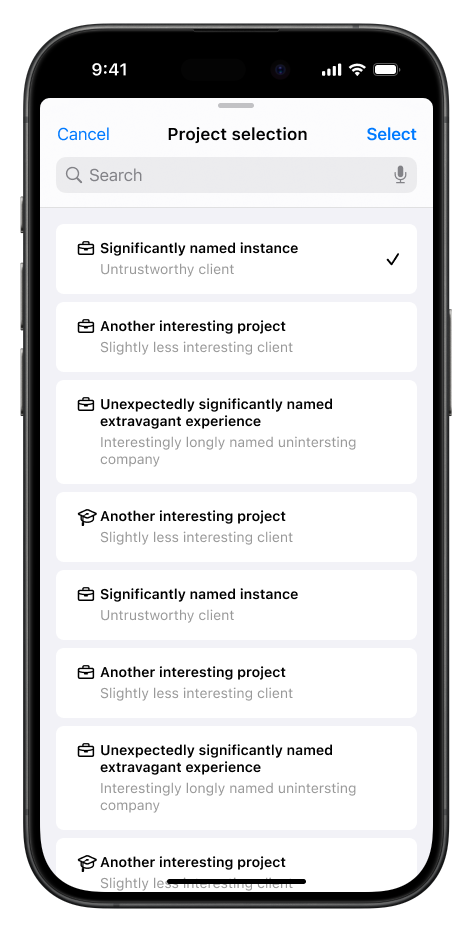
\includegraphics[width=6cm]{project-selection.png}
		\caption{Výběr projektu}
		\label{fig:project-selection}
	\end{subfigure}
	\caption{Hlavní obrazovka}
	\label{fig:timer-and-project-selection}
\end{figure}

Ovládací panel pro časovač může mít různé varianty, jak bude vypadat, podle toho, v~jakém je stavu. Návrh počítá se dvěma možnostmi, jak půjde přidávat časové záznamy do historie:
\begin{itemize}
\item Pomocí časovače – uživatel zapne časovač, když bude chtít začít měření, a poté ho vypne, když bude měření chtít ukončit, čímž se automaticky uloží záznam se zadanými vlastnostmi.
\item Ručně – uživatel ručně zadá začátek a konec záznamu a poté časový záznam uloží.
\end{itemize}
Ovládací panel půjde přepínat mezi těmito dvěma stavy pomocí vedlejšího tlačítka. Hlavní ovládací tlačítko bude vypínat/zapínat časovač, pokud bude přepnut do stavu časovače, nebo bude přidávat ruční záznam, pokud bude v~ručním stavu. V~ovládacím panelu časovače bude také možné vybrat projekt a popis, které budou k~danému záznamu přiděleny. Klik na volbu projektu otevře novou obrazovku, která umožní vyhledávání v~projektech a výběr projektu, jak lze vidět na obrázku \ref{fig:project-selection}. Různé stavy časovače (časovač/manuální, zapnutý/vypnutý, vyplněný/nevyplněný, atd.) lze nahlédnout v~obrázku \ref{fig:timer-control-variants}.

\begin{figure}[h]
	\centering
	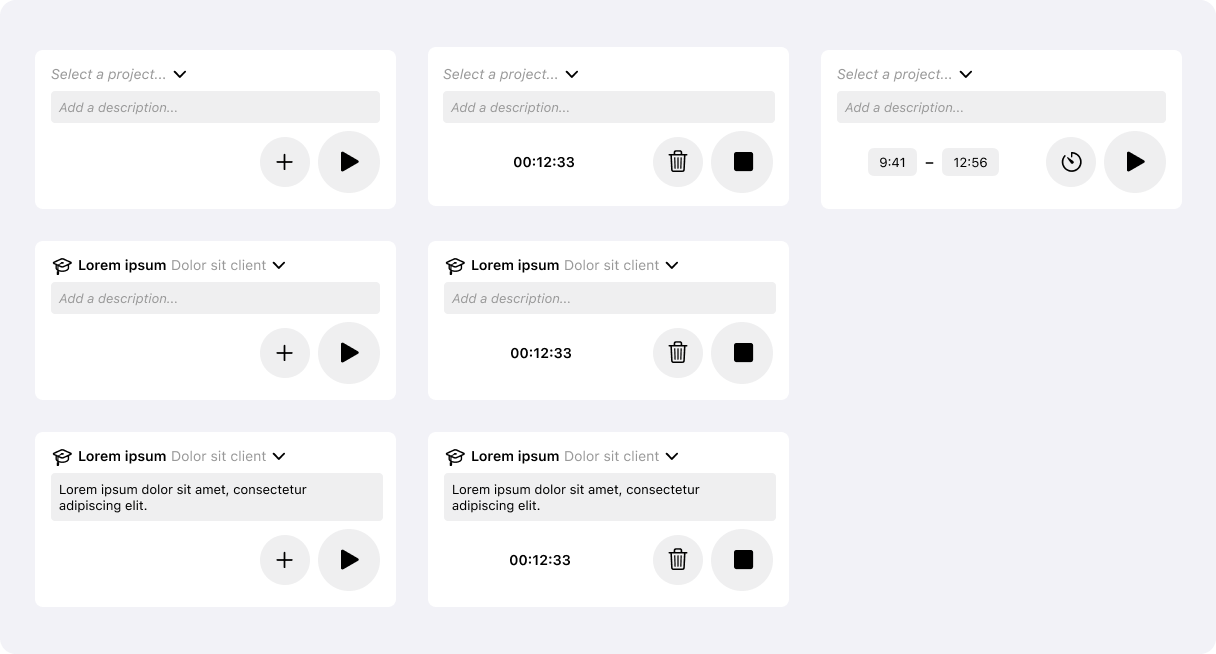
\includegraphics[width=\textwidth]{timer-control-variants.png}
	\caption{Různé stavy ovladače pro časovač}
	\label{fig:timer-control-variants}
\end{figure}

Na obrázku \ref{fig:timer} lze dále v~horní části obrazovky vidět souhrn časových záznam za tento den a týden. Uživatel tak uvidí, kolik času již odpracoval v~daný den i~týden. Časové záznamy v~historii budou také seskupeny podle dnů – každý den bude mít nadpis s~datem a součtem odpracovaného času za ten den. Jednotlivé záznamy také půjdou mazat pomocí posuvného gesta.

Vzhledem k~tomu, že v~historii se může časem nacházet mnoho záznamů, měla by tato obrazovka podporovat stránkování, tedy funkci, že nebude ze zdroje načítat všechny záznamy najednou, ale pouze nějaký kus (stránku), a postupně může načítat další, pokud si to uživatel bude přát. Pokud se během načítání objeví chyba, tak se na této obrazovce ovládací panel časovače ani historie záznamů vůbec nezobrazí – zobrazí se pouze popis chyby a tlačítko pro opakování pokusu o~načtení. Pokud uživatel zatím žádné záznamy mít nebude, tak nebude potřeba zobrazovat nějakou explicitní formu prázdné obrazovky – pouze bude ve spodní části obrazovky ovládací panel a nad tím prázdno.

U~obrazovky pro výběr projektu bude také explicitní chybový stav, který ukáže popis chyby včetně tlačítka pro opakování. Na této obrazovce už ale bude potřeba definovat i~prázdný stav, aby se zobrazila nějaká instrukce, že uživatel nemá vytvořené žádné projekty a musí si je vytvořit na místě k~tomu určeném (bude navrženo dále). Prázdná data lze ale ještě rozdělit do dvou kategorií – prázdná data kvůli tomu, že uživatel žádné projekty nemá, nebo prázdná data kvůli tomu, že jeho vyhledávání neodpovídá žádný projekt. Pro tyto dva stavy je potřeba použít rozdílné texty pro uživatele.

%---------------------------------------------------------------
\subsection{Profil uživatele}
%---------------------------------------------------------------

Poslední kartou v~navigační liště aplikace bude karta s~Profilem. Uživatel zde bude mít základní přehled a akce týkající se jeho účtu, jak lze nahlédnout na obrázku \ref{fig:profile-overview}. Uživatel se odsud dostane do seznamu klientů a seznamu profilů, dále si může pomocí tlačítka svůj účet smazat, nebo se odhlásit, což ho vrátí zpět na přihlašovací obrazovku \ref{fig:login}. Mazání účtu je nevratná akce, která vymaže spoustu dat spojených s~uživatelem, je tedy potřeba alespoň ukázat ověřující dialog, který lze nahlédnout na obrázku \ref{fig:profile-delete}. 

\begin{figure}[h]
    \centering
    \begin{subfigure}[b]{0.4\textwidth}
		\centering
		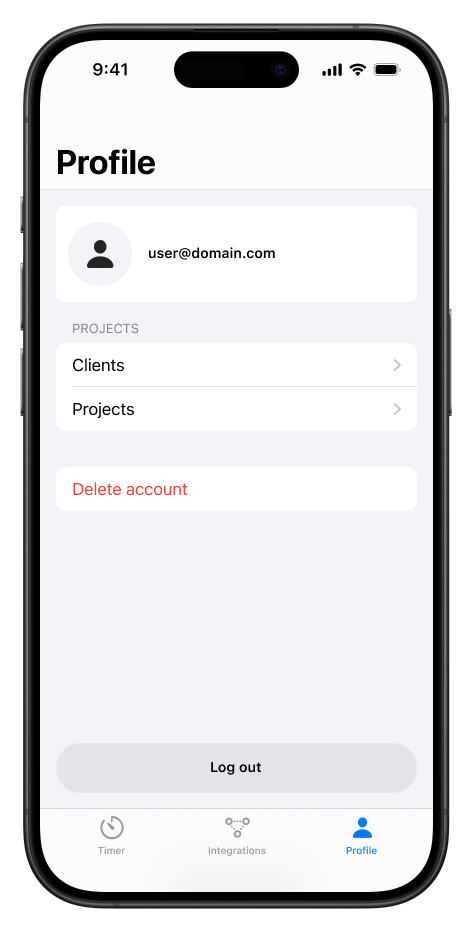
\includegraphics[width=6cm]{profile.png}
		\caption{Přehled}
		\label{fig:profile-overview}
	\end{subfigure}
	\hspace{2cm}
	\begin{subfigure}[b]{0.4\textwidth}
		\centering
		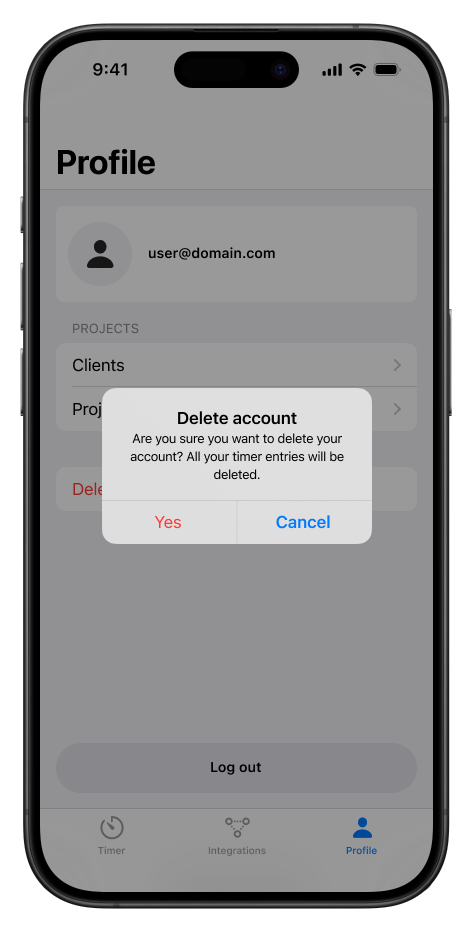
\includegraphics[width=6cm]{profile-delete.png}
		\caption{Smazání účtu}
		\label{fig:profile-delete}
	\end{subfigure}
	\caption{Profil}
	\label{fig:profile}
\end{figure}

V~horní části obrazovky se také nachází uživatelův e-mail, jako indikace toho, na kterém účtě je uživatel přihlášen.

Pokud uživatel klikne na tlačítko klientů, zobrazí se mu seznam jeho klientů, jak lze vidět na obrázku \ref{fig:client-list}. V~tomto seznamu může v~klientech vyhledávat, otevřít detail klienta, nebo vytvořit nového, pomocí tlačítka vpravo nahoře v~navigační liště. Při kliknutí na konkrétního klienta, s~cílem zobrazit jeho detail, i~při kliknutí na volbu tvorby nového klienta, se zobrazí stejná obrazovka detailu, kterou lze nahlédnout na obrázku \ref{fig:new-client}. V~případě zobrazení detailu již existujícího klienta se akorát změní název v~navigační liště, předvyplní se hodnoty klienta a zobrazí se navíc tlačítko pro smazání klienta.

Při tvorbě nebo úpravě klienta uživatel může zvolit jeho název. V~budoucnu je možné přidat další parametry, které by mohly být ke klientovi přiděleny. Kliknutím na tlačítko \emph{Uložit} v~navigační liště se upravený klient uloží a uživatel bude odnavigován zpět na seznam klientů. V~případě, že uživatel klikne na tlačítko zrušit, bude také odnavigován zpět na seznam, ale všechny změny budou zahozeny.

Seznam projektů by měl mít také definované stavy pro chybu a prázdná data. V~případě chyby se zobrazí popis chyby a tlačítko pro opakování, v~případě, že uživatel nemá žádné klienty, se zobrazí tato informace a instrukce k~tomu, aby si nějakého klienta vytvořil. Opět je také potřeba rozlišit mezi tím, zda se žádní klienti nezobrazují proto, protože žádní nejsou, nebo protože žádní nevyhovují vyhledávánému výrazu.

Detail klienta bude mít také explicitní chybový stav, ale prázdný stav zde potřeba není, jelikož existující klient musí mít data vždycky, a nový klient určitě žádná nemá, tudíž budou pole prázdná.

\begin{figure}[h]
    \centering
    \begin{subfigure}[b]{0.4\textwidth}
		\centering
		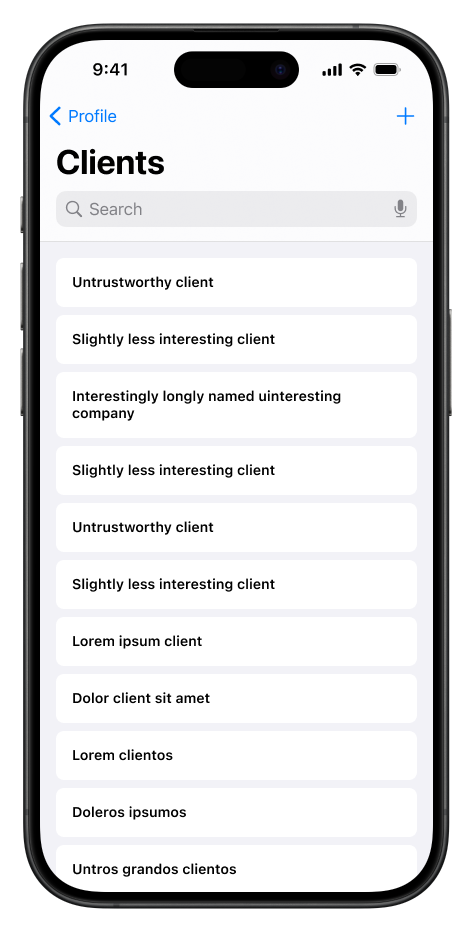
\includegraphics[width=6cm]{clients.png}
		\caption{Seznam}
		\label{fig:client-list}
	\end{subfigure}
	\hspace{2cm}
	\begin{subfigure}[b]{0.4\textwidth}
		\centering
		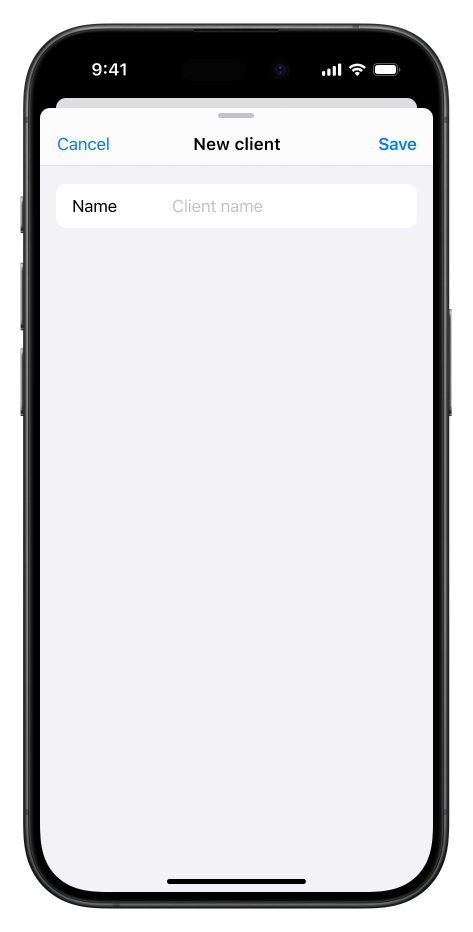
\includegraphics[width=6cm]{new-client.png}
		\caption{Nový klient}
		\label{fig:new-client}
	\end{subfigure}
	\caption{Klienti}
	\label{fig:clients}
\end{figure}

Seznam projektů a detail projektu funguje stejným způsobem, jako u~klientů. Kliknutí na tlačítko projektů v~profilu otevře seznam, odkud lze otevřít detail/tvorbu nového projektu. Seznam projektů lze nahlédnout na obrázku \ref{fig:project-list} a detail projektu na obrázku \ref{fig:new-project}.

Detail projektu narozdíl od klienta obsahuje více informací. Každý projekt musí patřit k~nějakému klientovi, tudíž je potřeba tohoto klienta zvolit, k~čemuž bude sloužit další obrazovka pro výběr klienta, která bude vypadat stejně, jako seznam klientů \ref{fig:client-list}, ale funkčně bude stejná, jako výběr projektu v~časovači \ref{fig:project-selection}. Dále je možnost nastavit jméno projektu, a poté nepovinný údaj o~typu projektu, což bude definovaný seznam hodnot, ze kterého půjde volit (\emph{Práce}, \emph{Škola} a další).

Chybové a prázdné stavy budou fungovat stejným způsobem, jako u~klientů.

\begin{figure}[h]
    \centering
    \begin{subfigure}[b]{0.4\textwidth}
		\centering
		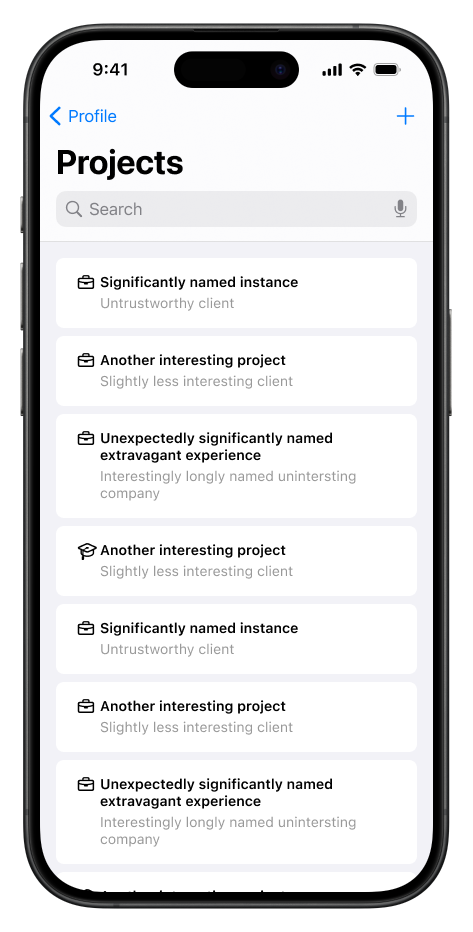
\includegraphics[width=6cm]{projects.png}
		\caption{Seznam}
		\label{fig:project-list}
	\end{subfigure}
	\hspace{2cm}
	\begin{subfigure}[b]{0.4\textwidth}
		\centering
		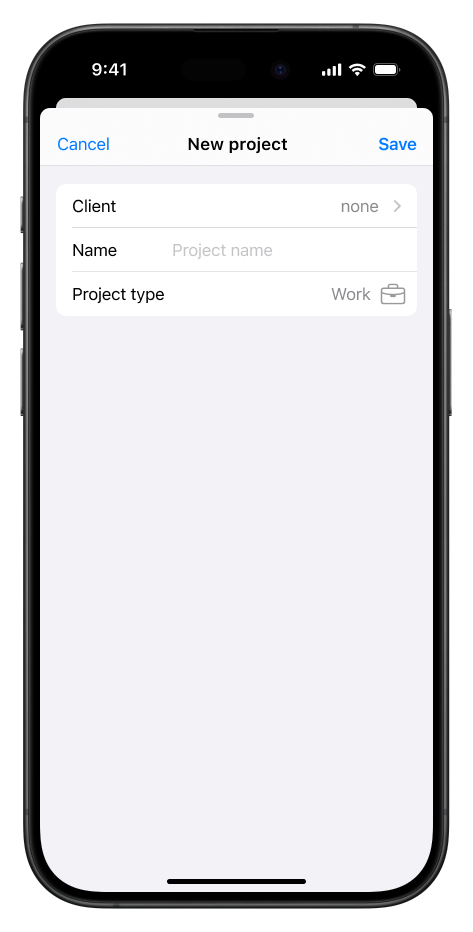
\includegraphics[width=6cm]{new-project.png}
		\caption{Nový projekt}
		\label{fig:new-project}
	\end{subfigure}
	\caption{Projekty}
	\label{fig:projects}
\end{figure}

%---------------------------------------------------------------
\subsection{Integrace}
%---------------------------------------------------------------

Jedním z~cílů práce je stanovit požadavky pro integraci spouštěčů měření času, dále požadavky na integraci aplikace s~existujícími systémy pro měření času, a tyto požadavky v~aplikaci implementovat. Tyto dva typy integrací lze rozdělit do skupin \emph{import} (integrace se spouštěči) a \emph{export} (integrace s~existujícími systémy).

%---------------------------------------------------------------
\subsubsection{Import}
%---------------------------------------------------------------

V~sekci \ref{tracking-triggers} byly popsány teoretické možnosti, s~jakými spouštěči by aplikace šla propojit.

Prvním typem spouštěčů měření času byly fyzické spouštěče, tedy nějaké fyzické formy ovladače. Z~uvedených příkladů v~analýze byl pouze jeden, který by uměl uskutečnit napojení na aplikaci napřímo, a to \emph{TIMEFLIP} \cite{timeflip}, který poskytuje protokol pro BLE komunikaci. Implementace BLE komunikace s~hardwarovým produktem je ale poměrně komplexní záležitost, která byla začleněna nad rámec rozsahu této práce, která se už takto věnuje návrhu a implementaci celé platformy pro měření odpracovaného času. Implementace tohoto typu komunikace tedy může být podnětem pro budoucí rozšíření aplikace.

Důležité ale je, aby na takové rozšíření byla aplikace dobře připravená, a aby minimálně poskytovala veřejné API umožňující se z~jakéhokoli budoucího konfigurovatelného hardwarového řešení na aplikaci napojit.

Dalším typem spouštěčů byly softwarové spouštěče, tedy nějaké formy automatizace. V~sekci \ref{software-tracking-triggers} zabývající se tomuto tématu bylo rozebráno několik typů automatizace (podle polohy, času, režimu soustředění, a podobně). Také bylo ale zmíněno systémové řešení pomocí aplikace \emph{Zkratky} \cite{ios-shortcuts-app}, které dokáže automatizaci všech těchto typů vytvořit. \emph{Zkratky} poskytují společné systémové API, které je velmi rozšířené a Apple se snaží vývojáře přesvědčit, aby nějakou část funkcionality aplikace na toto API napojili. Potenciál této platformy je velký, protože její API umožňuje propojování různých procesů navzájem, aplikace si můžou přeposílat výsledky jednotlivých procesů, navazovat na ně a pracovat s~nimi. 

Aplikace se mohou na toto API napojit pomocí definic takzvaných \emph{App Intents}. Apple v~jejich dokumentaci \cite{ios-app-intents} poskytuje podrobné informace k~tomu, jak tyto \emph{App Intents} definovat, jak pro ně vytvářet parametry, a další. Tyto struktury reprezentují nějakou akci aplikace, kterou uživatel může spustit. Nejpoužívanější (podle očekávání) automatizovatelné funkce aplikace budou zapínání časovače, vypínaní časovače a případně rušení časovače. Bylo by tedy vhodné pro tyto tři funkce vytvořit \emph{App Intents}, které uživatelům umožní vytvářet zkratky a automatizace pro jejich spuštění. V~případě zapínání časovače se také naskytuje možnost použití dvou nepovinných parametrů, a to projekt a popis, který bude uživatel chtít k~záznamu přiřadit.

Implementace integrace se systémovými zkratkami umožní širokou a potenciálně velmi rozšiřovatelnou míru integrace, protože se jedná o~společné systémové API, na které lze napojit jakoukoli aplikaci, a spousta aplikací nějakou formu napojení na zkratky implementuje. U~systémových aplikací to dokonce platí pro všechny – pokrytí automatizovatelných funkcí je zde velmi široké.

%---------------------------------------------------------------
\subsubsection{Export}
%---------------------------------------------------------------

V~sekci \ref{existing-tracking-solutions} byly popsány populární systémy \emph{Clockify}, \emph{Toggl Track} a \emph{Deputy}, které poskytují funkce pro zaznamenávání odpracovaného času. Všechny tyto systémy poskytují možnost importu dat z~CSV souborů, a u~\emph{Clockify} a \emph{Toggl Track} šlo o~velmi podobné formáty.

Možnost exportu z~aplikace do CSV souboru by tedy byla silným nástrojem, pomocí kterého by se záznamy z~aplikace mohly nejen importovat do těchto systémů, ale byla by uživatelům poskytnuta volná možnost, co s~exportovanými daty dělat. V~různých programech by si je mohli dle svého uvážení analyzovat, vizualizovat, a další. Možnost exportu dat do CSV souboru by tedy v~aplikaci neměla chybět. Ideálně by mělo jít o~formát, který půjde importovat jak do systému \emph{Clockify}, tak do systému \emph{Toggl Track}. Systém \emph{Deputy} cílí na trochu jinou cílovou skupinu, napojení na něj by proto nebylo tolik relevantní, jak již bylo popsáno v~sekci \ref{deputy}.

Všechny zmíněné systémy také poskytovaly veřejné API pro napojení na jejich struktury. Zde už se nepůjde spolehnout na nějaké obecné řešení, které bude pasovat na více systémů, ale bude se potřeba na každý systém napojit zvlášť. V~rámci implementace by mohla být vytvořena integrace alespoň s~jedním systémem, a zároveň by implementace mohla být připravena pro rozšíření o~napojení na další systémy.

Rozhraní pro integraci s~dalšími systémy bylo navrženo následovně. V~pořadí druhá, tedy prostřední, karta v~navigační liště bude sloužit pro vytváření integrací. Aby aplikace mohla v~budoucnu podporovat různé typy integrací a zároveň aby si uživatel mohl svá nastavení integrací ukládat, bude hlavní obrazovku integrací představovat seznam již vytvořených integrací, který lze nahlédnout na obrázku \ref{fig:integration-list}.

\begin{figure}[h]
    \centering
    \begin{subfigure}[b]{0.4\textwidth}
		\centering
		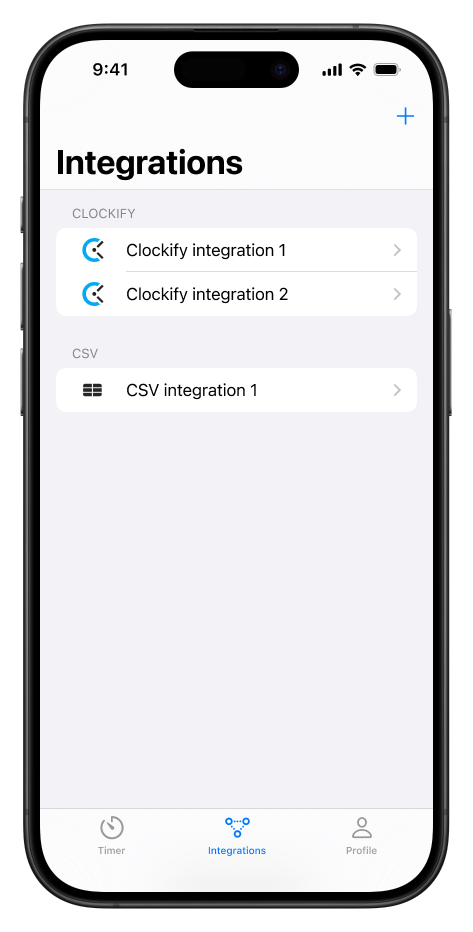
\includegraphics[width=6cm]{integrations.png}
		\caption{Seznam}
		\label{fig:integration-list}
	\end{subfigure}
	\hspace{2cm}
	\begin{subfigure}[b]{0.4\textwidth}
		\centering
		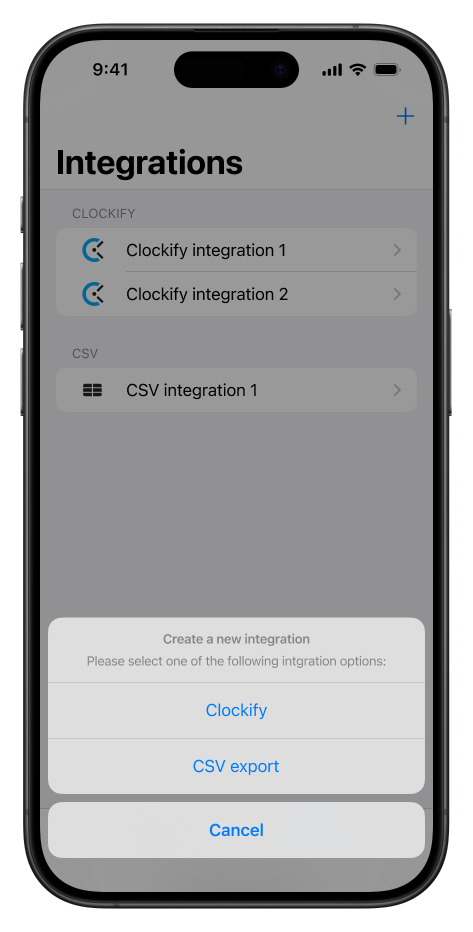
\includegraphics[width=6cm]{new-integration.png}
		\caption{Nová integrace}
		\label{fig:new-integration}
	\end{subfigure}
	\caption{Integrace}
	\label{fig:integrations}
\end{figure}

V~tomto seznamu budou prvky jednotlivých vytvořených integrací, které budou mít přidělenou ikonku podle toho, o~jaký typ integrace se jedná (CSV, \emph{Clockify}, a další). Vpravo nahoře v~navigační liště bude tlačítko pro přidání nové integrace, které otevře dialog s~možnostmi, jaký typ integrace chce uživatel vytvořit, jak lze nahlédnout na obrázku \ref{fig:new-integration}. Tento seznam bude mít definovaný chybový stav, kde se místo seznamu zobrazí popis chyby a tlačítko pro opakování, a prázdný stav, který zobrazí jen informaci o~tom, že si uživatel žádné integrace zatím nevytvořil.

Vytvoření nové integrace, nebo otevření detailu existující integrace, otevře obrazovku pro detail integrace, jak lze vidět na obrázku \ref{fig:clockify-integration}. Obrázek \ref{fig:clockify-integration} reprezentuje detail \emph{Clockify} integrace, u~které je potřeba nastavit název integrace, API klíč pro napojení na \emph{Clockify} účet a případně nějaké další parametry pro exportování dat. Tento detail se bude lišit pro různé typy integrací podle toho, jaké parametry budou pro exportování dat potřeba. Například u~exportu do CSV dat bude potřeba jen název a nic dalšího. Tato obrazovka bude potřebovat definic chybového stavu, který bude opět zobrazovat popis chyby a tlačítko pro opakování. Prázdný stav zde nemá smysl. Obrazovky pro vytvoření nové integrace, nebo pro úpravu existující integrace, se budou lišit akorát v~možnosti odstranění integrace – u~existující integrace se přidá tlačítko, které to umožní.

Kliknutí na tlačítko exportu dat otevře další obrazovku, která lze vidět na obrázku \ref{fig:export-data}. Tato obrazovka bude sloužit pro manuální export dat v~zadaném období. U~některých typů integrací totiž bude dávat smysl nabídnout automatický export dat, například u~\emph{Clockify} integrace, kde je možné každý nově vytvořený záznam rovnou automaticky exportovat do \emph{Clockify} účtu. Ale například u~exportu do CSV souboru taková automatizace nedává smysl, tento typ integrace bude tedy sloužit pouze pro manuální export. Tato obrazovka je poměrně jednoduchá, vyžaduje po uživateli pouze zadání od kdy a do kdy chce časové záznamy exportovat. Pokud zadá validní interval a klikne na tlačítko pro export, aplikace data exportuje. V~případě \emph{Clockify} integrace se pokusí data odeslat na \emph{Clockify} API, v~případě CSV integrace nabídne uživateli výsledný soubor, který si s~ním poté může dělat co chce – uložit do souborů, odeslat e-mailem, otevřít v~jiné aplikaci, atd. U~této obrazovky není potřeba definovat žádné chybové nebo prázdné stavy, protože samotná obrazovka žádná data nepotřebuje.

\begin{figure}[h]
    \centering
    \begin{subfigure}[b]{0.4\textwidth}
		\centering
		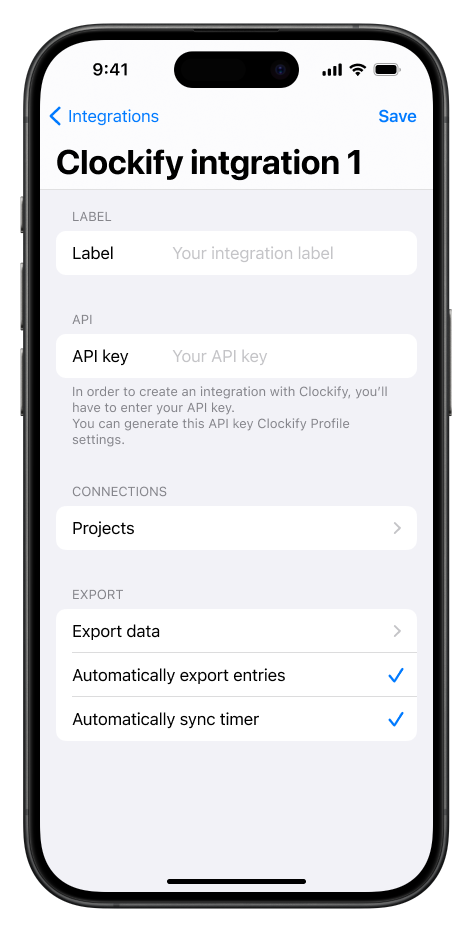
\includegraphics[width=6cm]{clockify-integration.png}
		\caption{Clockify integrace}
		\label{fig:clockify-integration}
	\end{subfigure}
	\hspace{2cm}
	\begin{subfigure}[b]{0.4\textwidth}
		\centering
		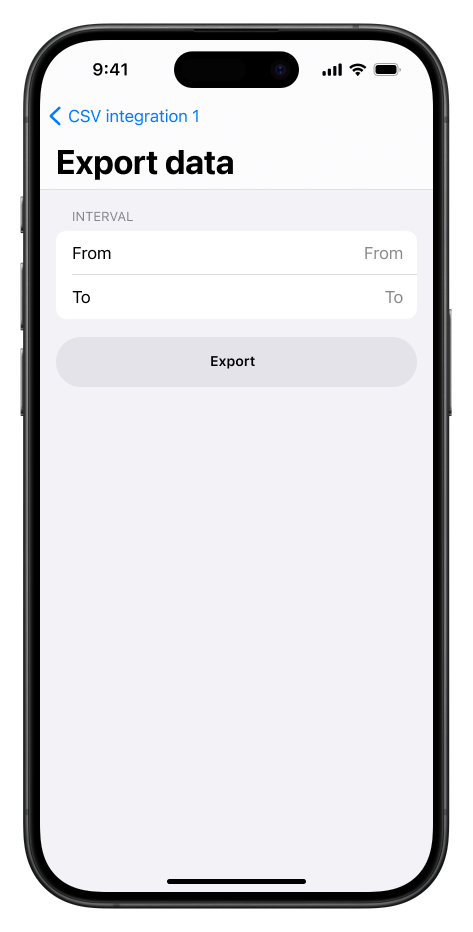
\includegraphics[width=6cm]{export-data.png}
		\caption{Export dat}
		\label{fig:export-data}
	\end{subfigure}
	\caption{Detail integrace}
	\label{fig:integration-detail}
\end{figure}

%---------------------------------------------------------------
\section{Architektura}
%---------------------------------------------------------------

V~analýze v~sekcích \ref{app-architecture}, \ref{crossplatform-multiplatform} a \ref{backend} byly popsány různé architektury pro mobilní aplikace, backendová řešení a databáze. Tato sekce se bude věnovat návrhu architektury celé platformy a nástrojů či jiných produktů, které budou potřeba pro realizaci aplikace.

%---------------------------------------------------------------
\subsection{Architektura platformy}\label{platform-architecture}
%---------------------------------------------------------------

V~první řadě je potřeba se rozhodnout, jakou architekturu bude mít celá platforma, tedy jaký přístup bude zvolen pro vývoj mobilní aplikace, jaké řešení bude zvoleno pro implementaci backendu a jaká bude zvolena implementace databáze. Kombinace těchto řešení lze seřadit na stupnici, která má dva konce:
\begin{itemize}
\item Outsourcování co největší části platformy na externí poskytovale (BaaS, DBaaS, atd.). Tento přístup by byl nejjednodušší z~hlediska komplexní a časové náročnosti implementace, ale ze své podstaty by byl nejvíce omezující ve flexibilitě a možnosti budoucích rozšíření. V~případě, že by bylo v~budoucnu rozhodnuto, že se například změní poskytovatel databáze, tak by bylo značně náročnější implementaci pro takovou změnu upravit. Zejména v~případě, kdyby na jednom externím poskytovateli záviselo více částí infrastruktury.
\item Vlastní implementace všech částí platformy. Toto by vyžadovalo vlastní implementaci nativní aplikace, backendu i~databáze. V~případě, že by bylo v~budoucnu rozhodnuto, že se aplikace rozšíří například o~Android aplikaci, musela by být implementována tato aplikace celá, ale zase by se jen napojila na existující backend. V~tomto ohledu je toto řešení nejvíce flexibilní. Předchozí příklad eventuální změny implementace databáze by byl mnohem jednodušší, pouze by se změnil zdroj dat v~implementaci backendu. Tento přístup by byl ale zásadně náročnější na komplexnost a časovou náročnost implementace. 
\end{itemize}

Vhodné řešení pro implementaci této aplikace bude pravděpodobně ležet někdy mezi těmito dvěma extrémy. Vzhledem k~tomu, že zadání aplikace vyžaduje implementaci aplikace pouze pro platformu iOS, nabízí se lákavé řešení implementovat pouze tuto nativní aplikaci a veškerý zbytek infrastruktury opravdu delegovat na nějaký BaaS. Z~osobních preferencí a kvůli solidní konkurenceschopnosti řešení a jeho obstání jako práce z~dílny oboru softwarového inženýrství se ale toto řešení zdá jako poněkud méně šťastné. Jako jedním z~vedlejších cílů této práce byla zvolena široká možnost budoucích rozšíření této aplikace. Potenciál, kam dále by se implementace dala rozšířit, je široký – aplikace by mohla být rozšířena o~již zmíněnou Android aplikaci, ale třeba také o~webovou aplikaci, nebo o nějakou administrátorskou variantu. Zmíněné řešení s~delegováním celé infrastruktury mimo nativní aplikaci na BaaS by jednoduché řešení těchto rozšíření moc neumožňovala, protože každé další napojení by muselo být implementováno úplně odděleně a muselo by se nějakým způsobem na BaaS napojit, čímž by navíc vznikla silná závislost na poskytovateli BaaS služby.

Zajímavou technologií, která byla zmíněna v~sekci \ref{crossplatform-multiplatform} je \emph{Kotlin Multiplatform} \cite{kotlin-multiplatform}. Z~osobního pohledu tato technologie činí ideální kompromis mezi maximálním využití funkcí jednotlivých platforem a snahy sdílení co největší části kódu. Tato technologie poskytuje nástroje pro sdílení kódu mezi aplikacemi pro různé platformy – iOS, Android, Web a další. Využití této technologie, přestože se realizace bude věnovat pouze implementaci pro platformu iOS, poskytne mnohem jednodušší možnosti pro budoucí rozšíření o~další platformy. Ve sdíleném kódu bude potřeba jen přidat nové moduly podle cílových platforem a bude možnost využít co největší část sdíleného kódu, který je společný pro všechny platformy. Použití této technologie je také osobní preferencí kvůli sympatiím s~jejím používáním, lehkou znalostí práce s~ní a možnost se s~touto technologií více seznámit napřímo.

Rozhodnutí využít technologie \emph{Kotlin Multiplatform} ovlivní i~rozhodnutí při volbě technologie pro implementaci backendu. Pro jazyk \emph{Kotlin} totiž existuje knihovna \emph{Ktor} \cite{ktor}, která poskytuje silné nástroje pro serverovou komunikaci. Poskytuje nástroje jak pro implementaci backendu, tak pro implementaci klienta a jejich vzájemnou komunikaci. Přestože tato knihovna není tak rozšířená a známá jako například \emph{Spring Boot} nebo \emph{Django}, které byly zmíněny v~sekci \ref{backend}, tak se ale hodí pro přehlednost a jednotu zdrojového kódu platformy, kde by celý backend i~multiplatformní část mohla být napsána v~jednom jazyce, v~jednom projektu, v~jednom společném repozitáři.

Rozhodnutí využít nástroje spojené s~multiplatformním vývojem v~\emph{Kotlinu} by se daly využít i~dále. Ve světě vývoje Android aplikací je poslední dobou častou volbou implementace uživatelského rozhraní pomocí knihovny \emph{Jetpack Compose} \cite{compose-ui}. Společnost \emph{JetBrains}, tvůrce technologie \emph{Kotlin Multiplatform}, vyvíjí technologii \emph{Compose Multiplatform} \cite{compose-multiplatform}, která dále umožňuje dokonce implementaci uživatelského rozhraní ve sdíleném kódu, které si narozdíl od cross-platformních řešení stále drží výhody multi-platformního přístupu, tedy lepšího využití možností dané platformy. Tato technologie je ale ve fázi \emph{Alpha} a není tolik pokročilá. Z~toho důvodu zůstala volba pro implementaci uživatelského rozhraní na nativním moderním přístupu s~pomocí knihovny \emph{SwiftUI} \cite{swiftui}.

Zatím tedy padly následující volby – nativní uživatelské rozhraní s~pomocí jazyka \emph{Swift} a knihovny \emph{SwiftUI}, multi-platformní implementace sdíleného kódu s~pomocí technologie \emph{Kotlin Multiplatform}, backend s~pomocí jazyka \emph{Kotlin} a knihovny \emph{Ktor}. Nyní ještě zbývá volba pro implementaci databáze.

V~tomto směru už bylo rozhodnuto, že využití externího DBaaS poskytovatele bude na místě. Toto řešení zjednoduší implementaci aplikace o~technologii vlastní databáze, ale stále si udrží možnost eventuální volby, kdy by se poskytovatel databáze mohl změnit. Jelikož bude mít platforma vlastní backend, nebude problém technologii databáze změnit z~externího poskytovatele například na technologii \emph{PostgreSQL}, protože už to bude jen otázka změny zdroje a migrace dat, zatímco implementace byznysové logiky a dalšího, která bude na backendu, zůstane stejná.

Jako dobrá volba externího poskytovatele BaaS se jeví \emph{Firebase} \cite{firebase} od firmy \emph{Google}. Jedná se o~rozšířenou technologii používanou mnoha aplikacemi. Tato technologie zároveň umožní obsluhu jiných funkcionalit aplikace, jako například autentizace. Není potřeba mezi implementací databáze a autentizace tvořit nějakou závislost, přijde-li tedy v~budoucnu požadavek poskytovatele autentizace nebo databáze změnit, může tak být učiněno nezávisle na sobě, tedy klidně pouze jedno z~toho, nebo obojí.

Tato volba architektury platformy dodržuje požadavek na velkou míru flexibility a rozšiřovatelnosti, zároveň se snaží zjednodušit náročnost implementace a eliminovat duplikace kódu, bude-li aplikace rozšířena o~další platformy. Schéma této architektury lze nahlédnout na obrázku \ref{fig:architecture}. V~tomto obrázku jsou také znázorněny možnosti případného rozšíření aplikace. Z~této celkové architektury platformy lze poté navrhovat architekturu jednotlivých částí.

\begin{figure}[h]
	\centering
	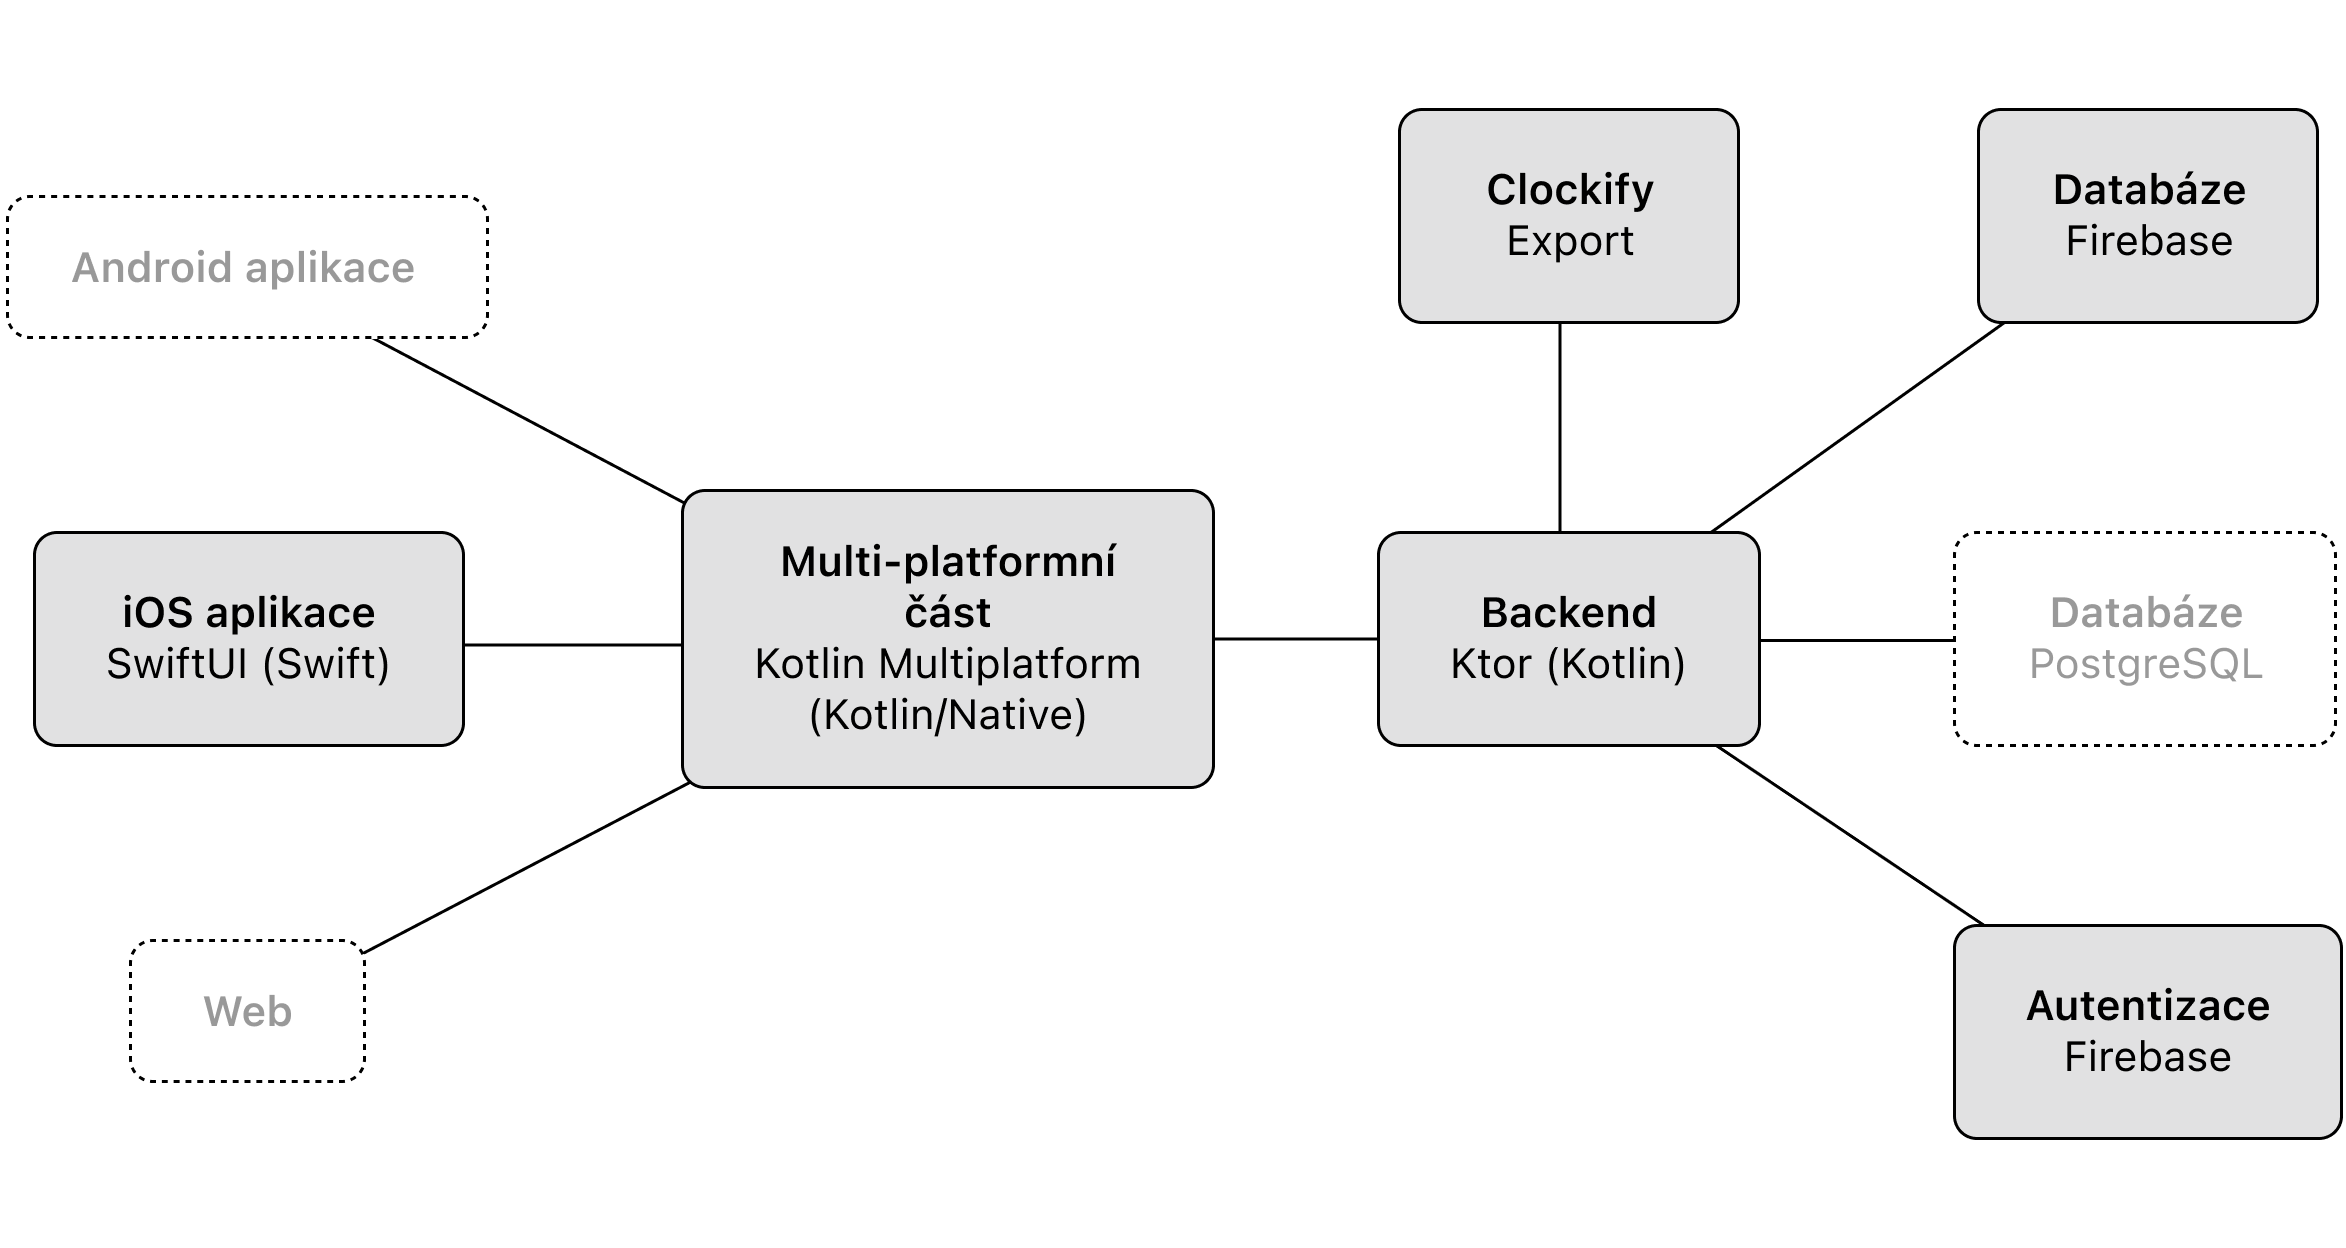
\includegraphics[width=\textwidth]{architecture.png}
	\caption{Architektura platformy}
	\label{fig:architecture}
\end{figure}

%---------------------------------------------------------------
\subsection{Architektura nativní aplikace}
%---------------------------------------------------------------

Architektura nativní aplikace bude vycházet z~veřejné šablony pro projekt mobilní aplikace pro platformy iOS a Android s~použitím technologie \emph{Kotlin Multiplatform}, nazvané \emph{Matee KMP DevStack} \cite{matee-devstack}. Důvody k~použití této platformy jsou osobní preference a znalost tohoto projektu. Alternativou by bylo například použití generátoru šablon projektů \emph{Kotlin Multiplatform Wizard} \cite{kmp-wizard}, ale \emph{DevStack} společnosti \emph{Matee} obsahuje velkou řadu užitečných nástrojů pro uživatelské rozhraní a další užitečné komponenty.

\emph{Matee DevStack} používá architekturu \emph{Clean Architecture} popsanou v~sekci \ref{app-architecture}. Technologie \emph{Kotlin Multiplatform} do této architektury zapadá tak, že nativní aplikace implementuje celou prezentační vrstvu, a multi-platformní část implementuje co největší možnou část doménové a datové vrstvy. Multi-platformní část je do nativní aplikace přidána jako knihovna, která je závislostí doménové vrstvy. Nativní aplikace má tedy přístup hlavně k~doménovým modelům a \emph{Use Cases}.

Nativní aplikace využívá \emph{modularizaci}, která představuje další vlastnost architektury, ve které je aplikace rozdělená do několika modulů, v~tomto případě podle funkcionalit. Prezentační vrstva aplikace tedy bude disponovat moduly podle funkcí jako \emph{Onboarding} (přihlášení/registrace), \emph{Timer} (časovač, historie záznamů), \emph{Integrations} (nastavení integrací), \emph{Profile} (profil uživatele) a poté například modulem \emph{UIToolkit}, který definuje společné komponenty pro prezentační vrstvu.

Doménová vrstva nativní aplikace bude obsahovat moduly \emph{SharedDomain}, což je modul, který definuje společné atributy domény aplikace, ale zde bude mít hlavní funkci jako poskytovatel sdílené knihovny, která bude výstupem multi-platformní části. Dále bude vrstva obsahovat modul \emph{Utilities}, který definuje užitečné nástroje pro práci s~doménovými či sdílenými funkcemi a objekty.

Datová vrstva obvykle obsahuje implementace repozitářů, v~modulech podle funkcionalit, a \emph{Providers}, také v~modulech podle funkcionalit. Jelikož většinu této vrstvy bude implementovat sdílený kód, bude tato vrstva obsahovat jen ty části, které sdílený kód implementovat nemůže. Což jsou obvykle platformní záležitosti, jako obsluha notifikací, GPS polohy, a další. Mohou to být ale i~další implementace, pro které zkrátka multi-platformní část nemá podporu, jako třeba různé funkce poskytovatele \emph{Firebase}. Tyto části kódu budou fungovat tak, že v~multiplatformní části kódu se budou nacházet rozhraní pro funkcionality, které musí implementovat každá platforma sama. V~multiplatformní části se bude pracovat s~těmito rozhraními, a nativní aplikace bude zodpovědná za to, že rozhraním poskytne implementace. Nativní aplikace tedy bude implementovat pouze tu část, kterou sdílená část implementovat nemůže, a výstupy těchto implementací bude vracet do sdíleného kódu.

Zmíněné moduly jsou v~nativní aplikaci ve skutečnosti balíčky typu \emph{Swift Package}, které jsou spravovány nástrojem \emph{Swift Package Manager} \cite{spm}. Nativní aplikace dále obsahuje aplikační vrstvu, která obsahuje základní části aplikace, jako \emph{AppDelegate}, \emph{Info.plist}, ikonu aplikace, nebo například rodičovský \emph{Flow Controller} aplikace, obvykle \emph{AppFlowController}, ze kterého se vytváří všechny další navigační toky. Architekturu nativní aplikace lze nahlédnout na obrázku \ref{fig:app-architecture}.

\begin{figure}[h]
	\centering
	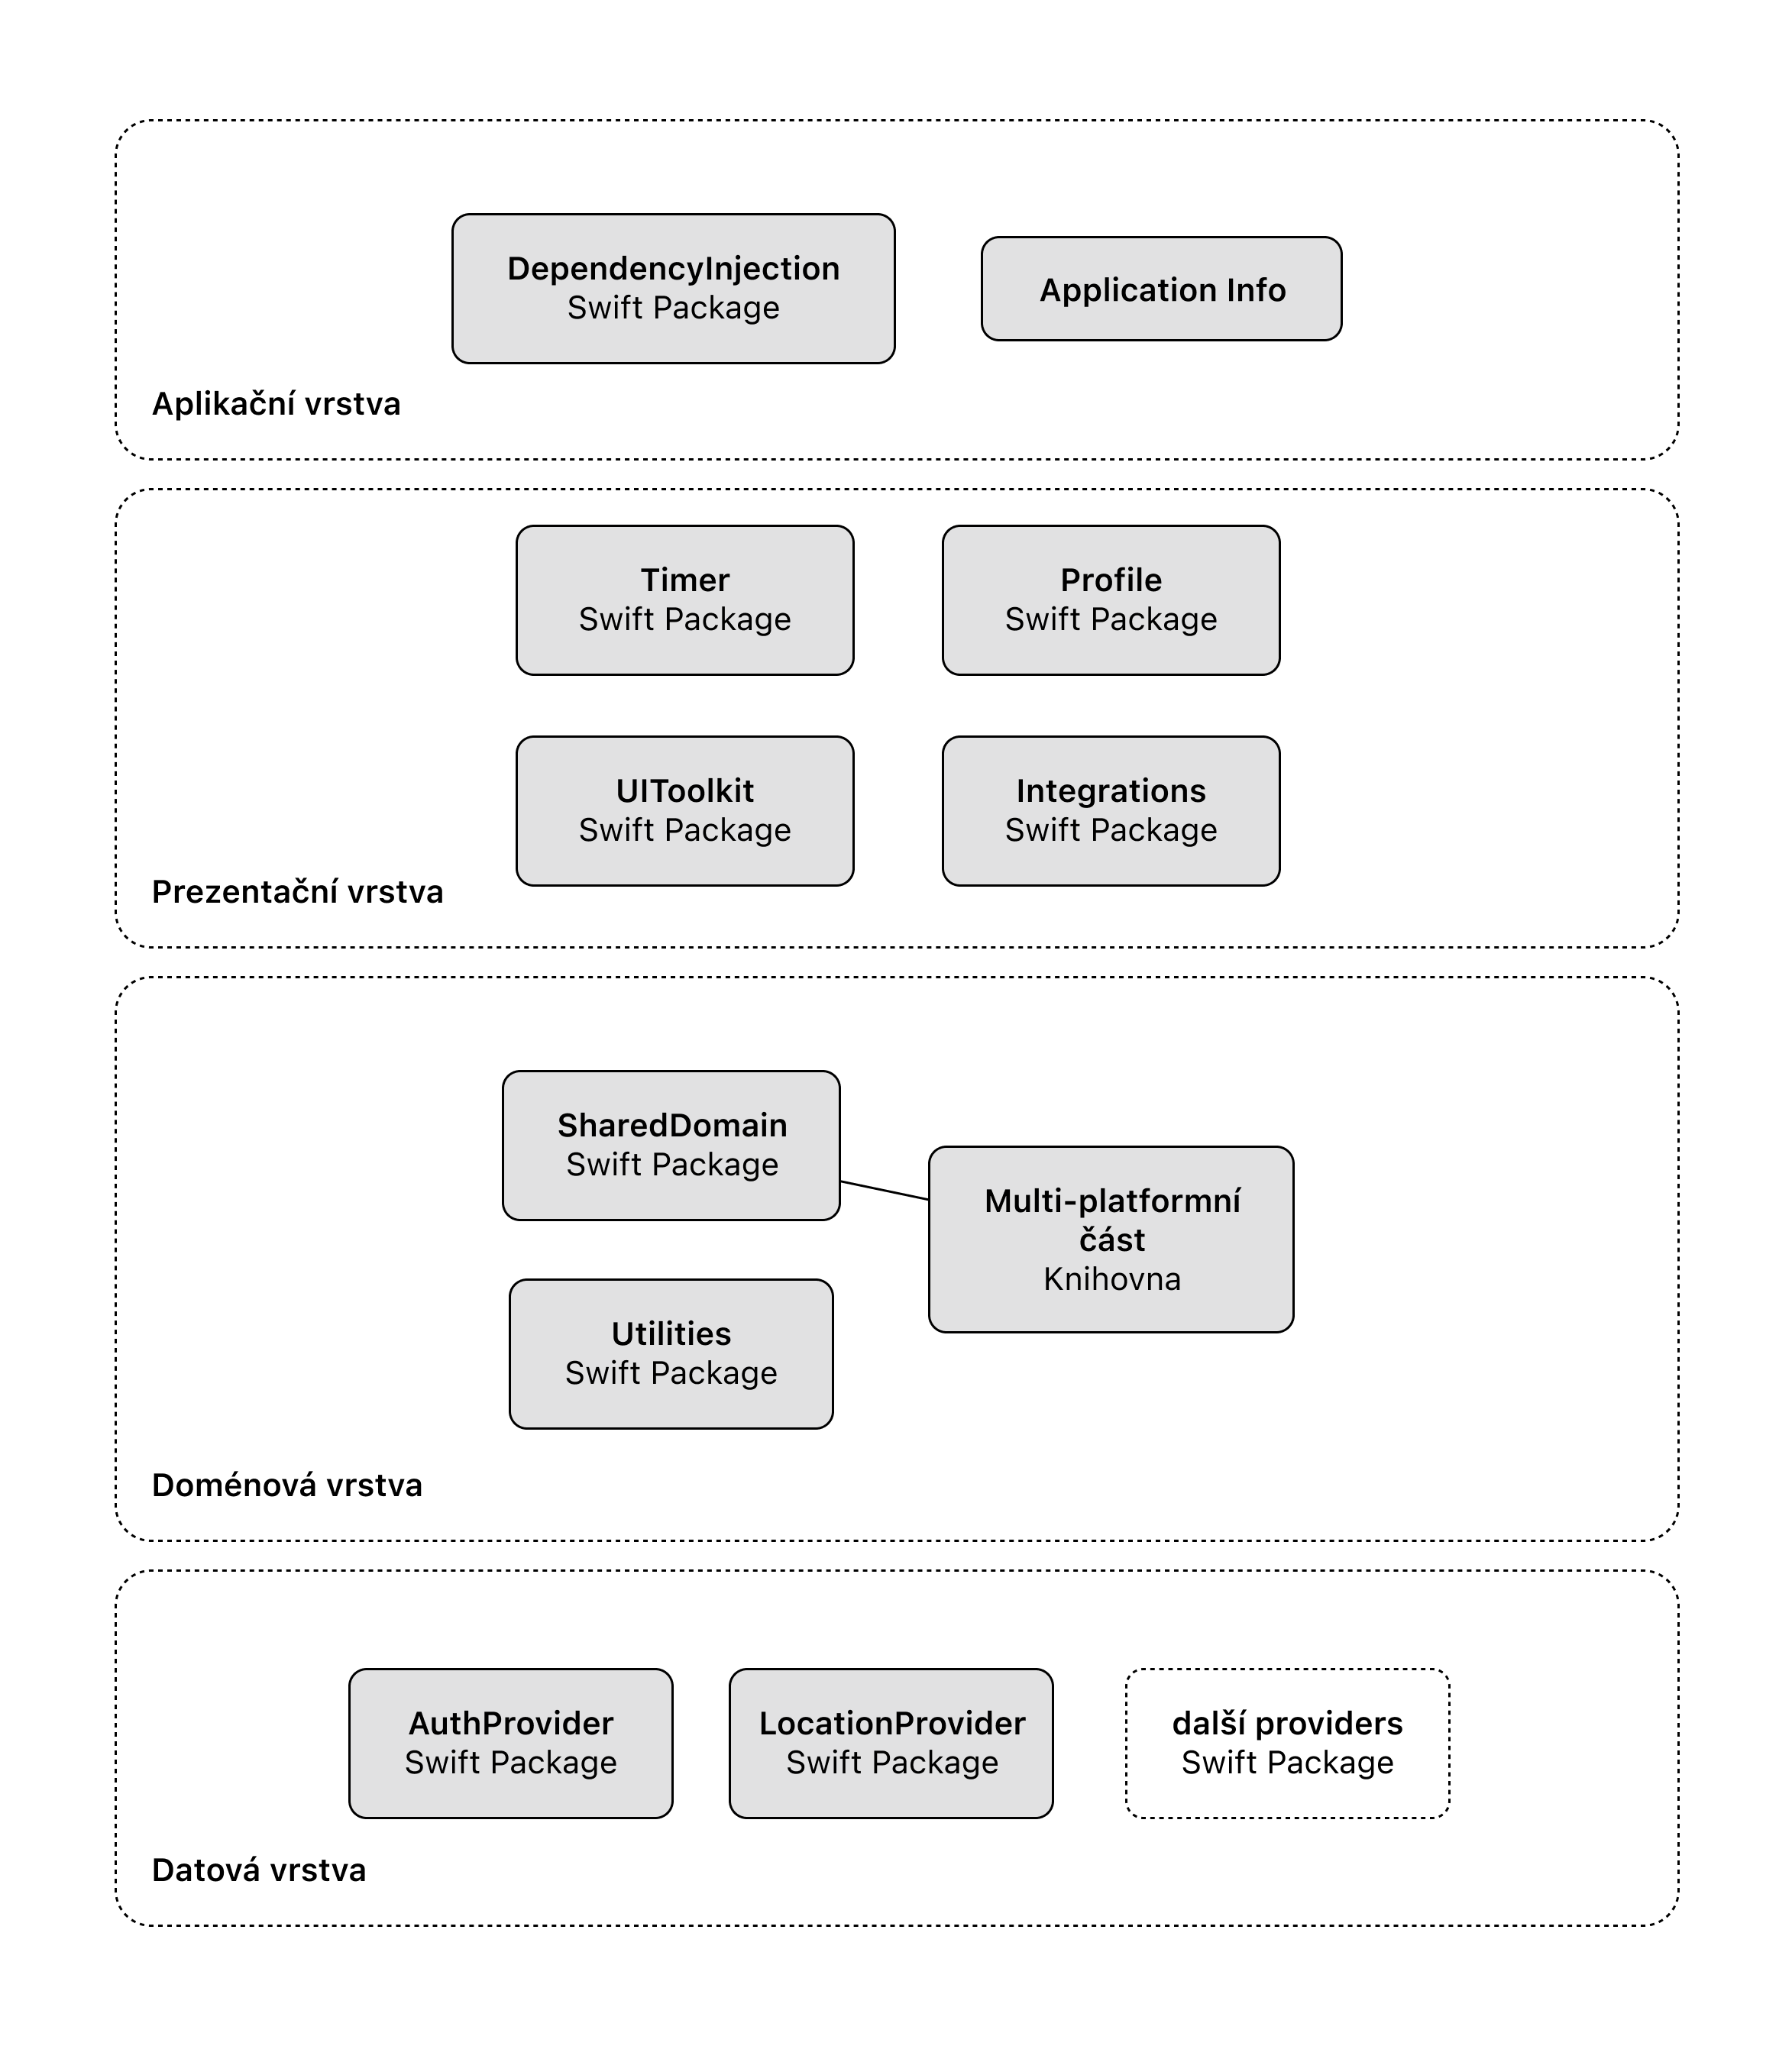
\includegraphics[width=\textwidth]{app-architecture.png}
	\caption{Architektura nativní aplikace}
	\label{fig:app-architecture}
\end{figure}

%---------------------------------------------------------------
\subsection{Architektura multi-platformní části}
%---------------------------------------------------------------

Multi-platformní část je rozdělena do dvou modulů – \emph{commonMain} a \emph{iosMain}. \emph{commonMain} obsahuje sdílený kód všech platforem, a \emph{iosMain} obsahuje kód, který se kompiluje pouze, pokud je cílovou platformou iOS. Toho se využívá speciálními klíčovými slovy v~\emph{Kotlinu} – \texttt{expect} a \texttt{actual}. Funguje to podobně, jako rozhraní – \emph{commonMain} definuje rozhraní funkce/třídy pomocí \texttt{expect}, a platformní modul definuje implementaci pomocí \texttt{actual}. Modul \emph{iosMain} má totiž přístup k~některým platformním API, ke kterým sdílený modul přístup nemá.

Modul \emph{commonMain} poté dodržuje stejnou architekturu, jako nativní aplikace, tedy \emph{Clean Architecture} s~\emph{modularizací} podle funkcionalit aplikace. Jediný rozdíl oproti architektuře používané v~nativní aplikace a popsané v~sekci \ref{app-architecture} je ten, že \emph{Providers} se ve světě \emph{Kotlinu} nazývají \emph{Sources}, ale jejich význam je identický.

Pokud bude v~budoucnu přidána podpora pro další platformy (Android, Web, \dots), bude potřeba v~multi-platformní části přidat konkrétní modul, například \emph{androidMain}. Tyto platformní moduly musí implementovat jen ty části, které jsou specifické pro platformu a \emph{Kotlin/Native} API k~nim má přístup. Dalším specifikem \texttt{expect} a \texttt{actual} je to, že pokud je v~\emph{commonMain} v~nějakém balíčku použito klíčové slovo \emph{expect}, tak v~platformním modulu potom musí být jeho \texttt{actual} implementace ve stejném balíčku. Tedy pokud je například \texttt{expect someFunction(param: String): String} v~balíčku \texttt{com.some.path}, tak implementace potom musí být také v~tomto balíčku. Tím pádem potom musí automaticky platformní moduly reflektovat strukturu aplikace, která je v~\emph{commonMain}.

%---------------------------------------------------------------
\subsection{Architektura backendu}
%---------------------------------------------------------------

Architektura backendu byla zvolena tak, aby byla v~souladu s~\emph{Clean Architecture}, která je používána v~nativní aplikaci i~v~multi-platformní části. Datové a doménové vrstvy jsou tedy identické, s~jednou výjimkou, že v~doménové vrstvě nejsou \emph{Use Cases}, ale ve vyšších vrstvách se budou používat \emph{Repositories} napřímo. To zejména proto, že na backendu mají \emph{Use Cases} menší smysl, než v~aplikaci. Ale nic by nebránilo tomu je také používat. Prezentační vrstva zde bude obsahovat \emph{Routes}, tedy \emph{Endpoints}, se kterými bude moct apikace komunikovat. Jednotlivé \emph{Endpoints} budou přímo volat \emph{Repositories}.

%---------------------------------------------------------------
\subsection{Architektura dat}
%---------------------------------------------------------------

S~ohledem na typ databáze, která byla pro platformu zvolena, je potřeba stanovit nějaké schéma dat. \emph{Firebase} nabízí dva typy databází – \emph{Cloud Firestore} a \emph{Realtime Database}. Oba typy jsou \emph{NoSQL} databáze, \emph{Cloud Firestore} je dokumentová databáze, která ukládá data jako kolekce dokumentů. \emph{Realtime Database} ukládá data v~jednom velkém JSON stromu. Vzhledem k~tomu, že \emph{Cloud Firestore} disponuje oproti \emph{Realtime Database} řadou výhod a je doporučenou variantou, bude tato databáze zvolena pro potřeby aplikace Trackee. \cite{rtdb-vs-firestore}

Jak již bylo řečeno, bude se jednat o~dokumentovou databázi. Pro potřeby aplikace bude nutné definovat následující objekty:
\begin{itemize}
\item\textbf{Klient} – Bude obsahovat informace o~klientovi, v~základní variantě jméno. V~budoucnu může být přidáno více atributů.
\item\textbf{Projekt} – Bude obsahovat informace o~projektu. Projekt musí patřit k~nějakému klientovi, takže bude muset obsahovat identifikátor klienta, ke kterému patří. Dále bude obsahovat jméno a nepovinně typ projektu. V~budoucnu také může být přidáno více atributů.
\item\textbf{Typ projektu} – Předdefinovaný seznam hodnot, například \emph{Práce} nebo \emph{Škola}.
\item\textbf{Uživatel} – Bude obsahovat informace o~uživateli. Identifikátorem uživatele bude \texttt{uid} (User ID), které by mělo být sdíleno s~identifikací v~autentizaci. Dále bude uživatel obsahovat informace o~svém časovači. Poté bude potřeba držet informace o~tom, jaké klienty a projekty má uživatel přiřazené. To by šlo ukládat například pomocí vnořené kolekce, kde bude jednotlivý dokument odpovídat klientovi, a tento dokument bude obsahovat pole hodnot, kterými budou identifikátory projektů, které má od daného klienta přiřazené. A nakonec bude ještě uživatel muset obsahovat data o~svých vytvořených integracích. Ty mohou být uloženy v~další kolekci, kde jednotlivý dokument bude odpovídat integraci.
\item\textbf{Data časovače} – Informace o~tom, jaký má vybraný projekt, popis, zda časovač běží a případně od kdy běží.
\item\textbf{Integrace} – Bude obsahovat název, typ a případně další atributy relevantní k~typu integrace.
\item\textbf{Typ integrace} – Prozatím \emph{CSV} nebo \emph{Clockify}.
\item\textbf{Časový záznam} – Prvek historie časových záznamů, který bude obsahovat informace zadané v~časovači. Tím je tedy vybraný projekt, popis, čas začátku a čas konce.
\end{itemize}
Klient, Projekt, Integrace a Časový záznam budou mít implicitně své identifikátory. U~Uživatele bylo již zmíněno, že jeho identifikátorem bude \texttt{uid}.

Dále je tedy potřeba navrhnout schéma dat. Jelikož se jedná o~dokumentovou databázi, je potřeba ho navrhnout tak, aby nevznikaly zbytečné duplicity a aby byla potřebná data lehce přístupná. Navržené schéma lze nahlédnout na obrázku \ref{fig:data-schema}. 

Schéma je navrženo tak, aby základní objekty byly ukládány ve vlastních top-level kolekcích (\emph{users}, \emph{clients}, \emph{projects} a \emph{entries}). Kolekce \emph{users}, respektive \emph{clients}, obsahují přímo dokumenty jednotlivých uživatelů, respektive klientů, podle jejich identifikátoru. Ale protože \emph{projects} vždy patří k~nějakému klientovi, respektive \emph{entries} k~nějakému uživateli, mají ještě jejich top-level kolekce vnořené kolekce v~dokumentech podle identifikátoru jejich klienta, respektive jejich uživatele. Alternativním přístupem by bylo \emph{projects}, respektive \emph{entries}, ukládat přímo do dokumentů jednotlivých \emph{clients}, respektive \emph{users}, ale tímto způsobem budou dokumenty odlehčeny od obsahování tolika dat a všechny nejpoužívanější objekty domény budou mít své top-level kolekce.

\begin{figure}[h]
	\centering
	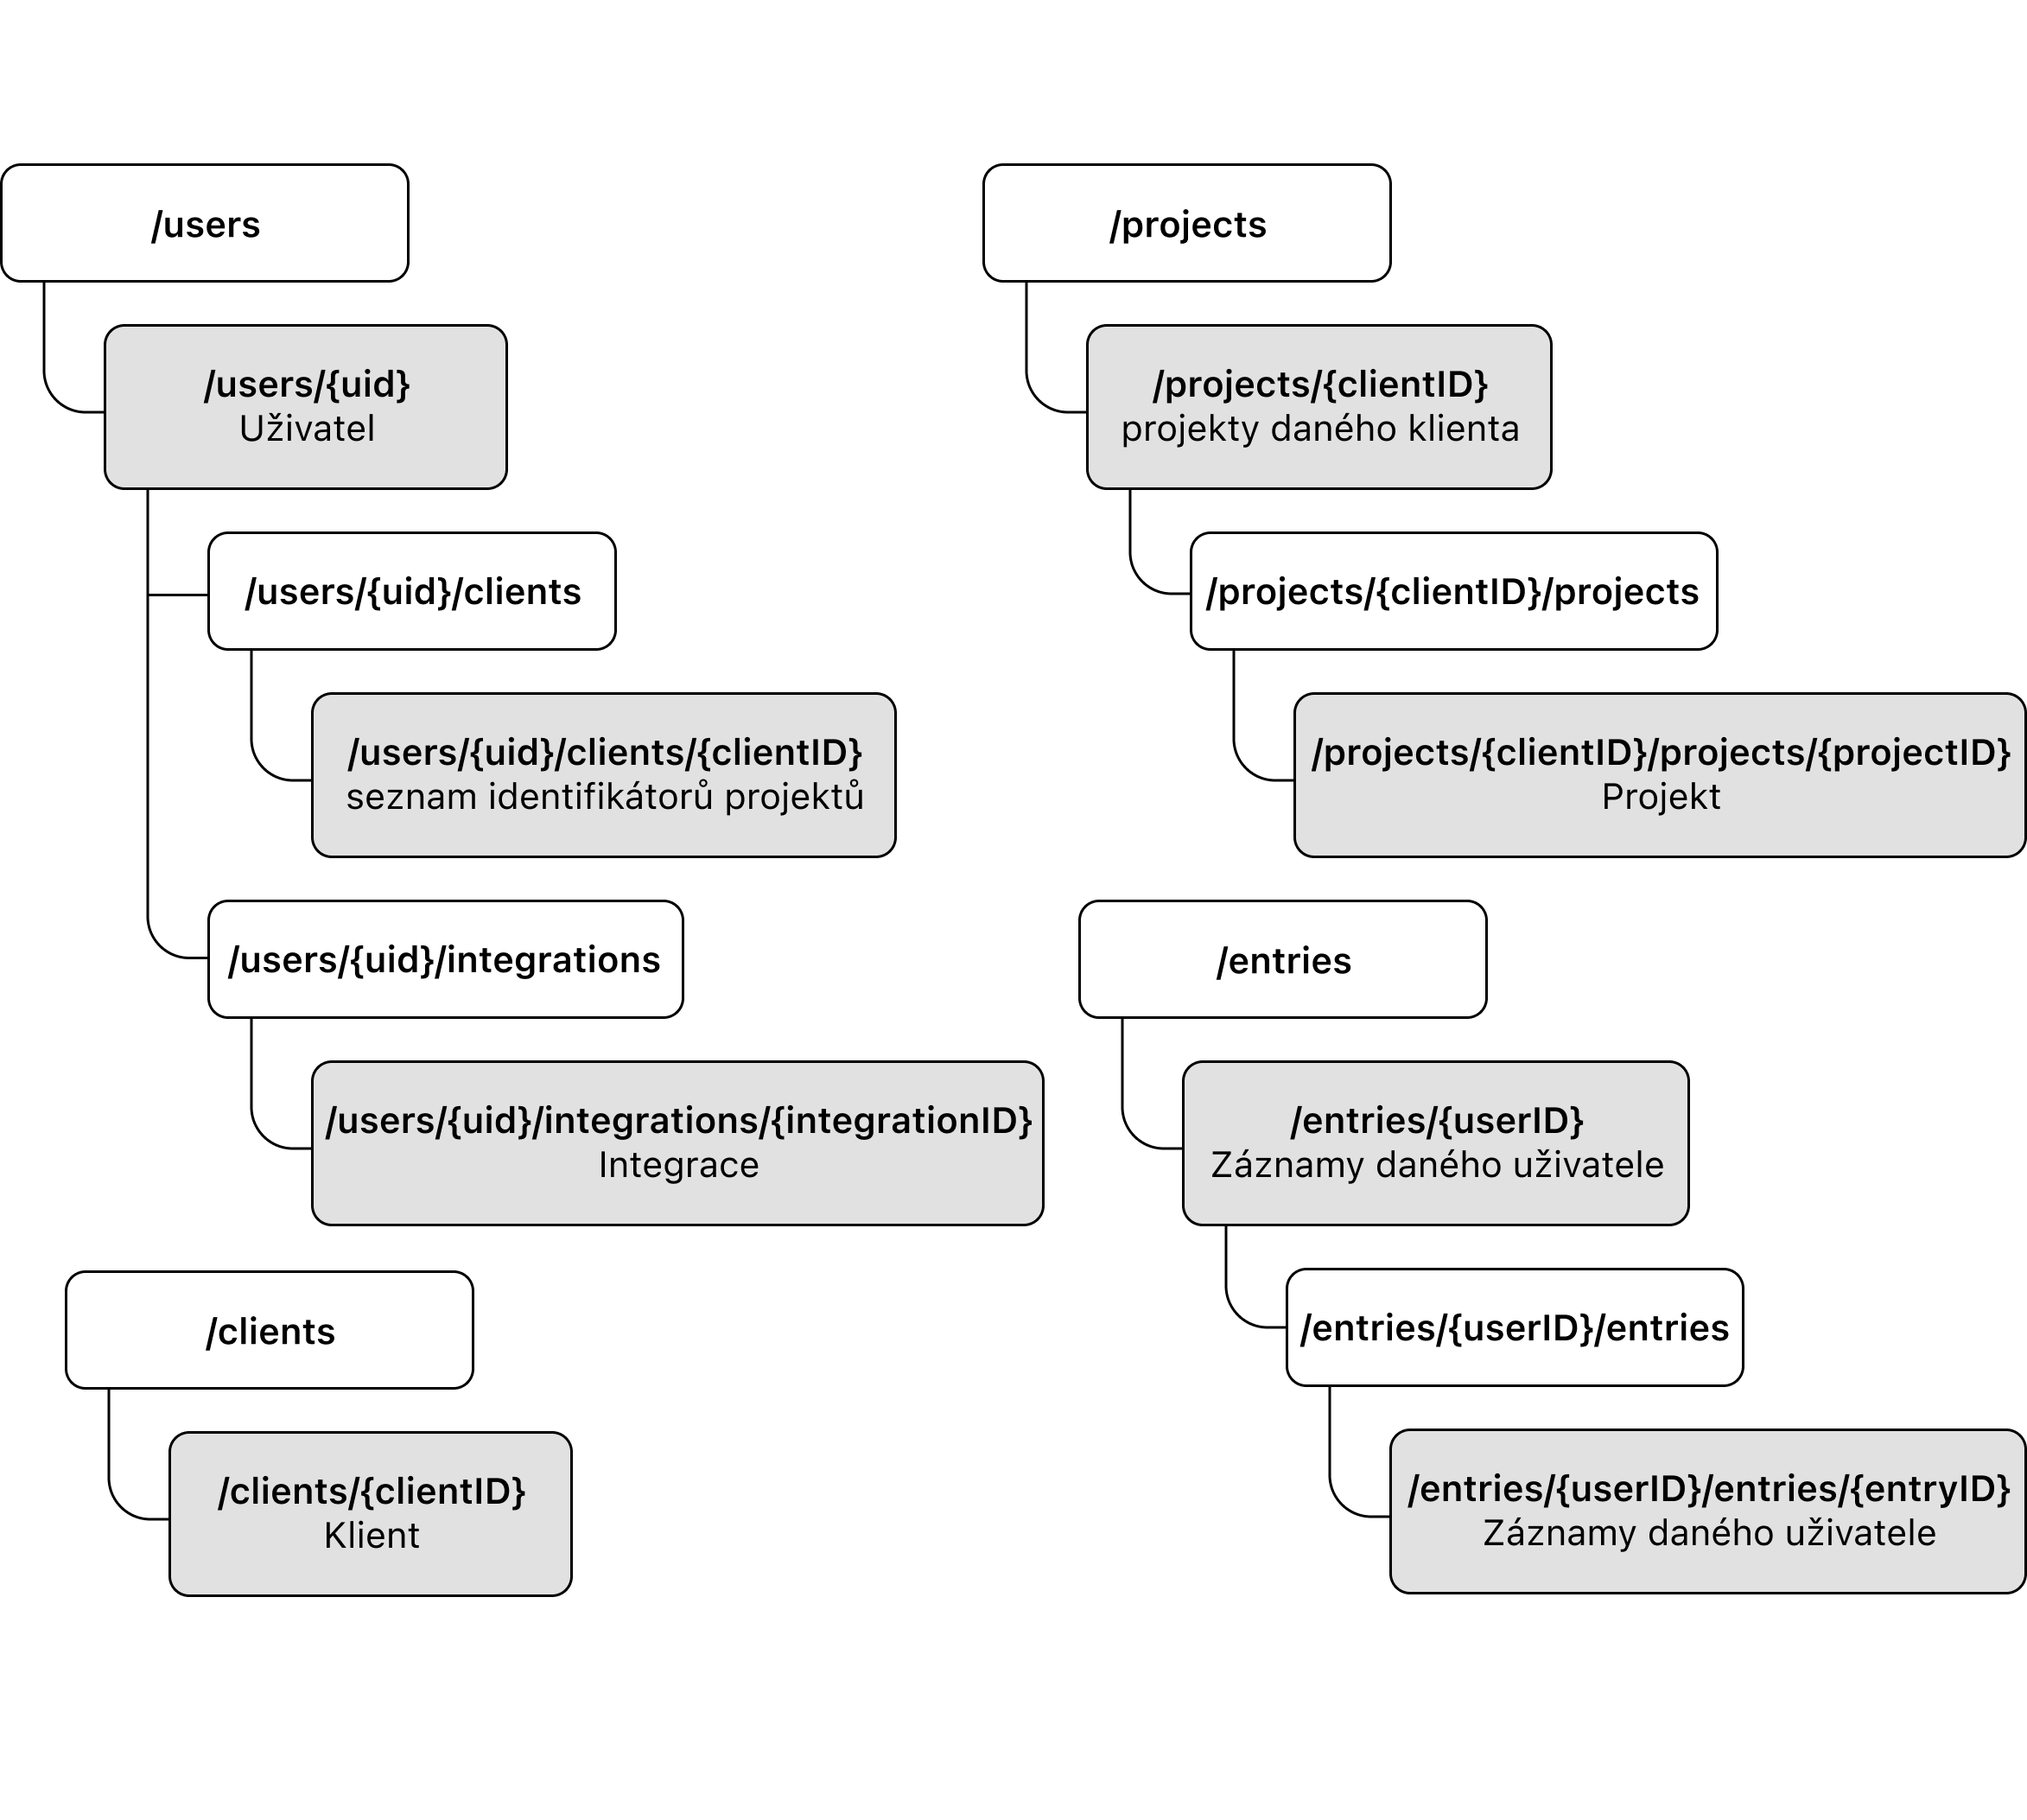
\includegraphics[width=\textwidth]{data-schema.png}
	\caption{Schéma dat}
	\label{fig:data-schema}
\end{figure}

%---------------------------------------------------------------
\section{Nástroje potřebné pro realizaci}\label{dev-tools}
%---------------------------------------------------------------

Před začátkem implementace je také potřeba navrhnout nástroje, které budou pro realizaci potřeba.

U~vývoje nativní aplikace není moc široký výběr vývojových nástrojů, jelikož jediné oficiální vývojové prostředí pro platformu iOS je \emph{Xcode}, popsané v~sekci \ref{ios-dev-tools}, které podporuje pouze operační systém \emph{macOS}. Toto vývojové prostředí obsahuje software pro podporu všech potřebných nástrojů, které jsou pro vývoj pro platformu iOS potřeba – kompilace, archivace, simulátory mobilních zařízení, debugger a další.

Pro vývoj multi-platformní části a backendu bude použito populární vývojové prostředí \emph{IntelliJ IDEA} společnosti \emph{JetBrains} \cite{intellij}. Toto IDE bylo zvoleno z~osobních preferencí a jeho dobré podpoře technologie \emph{Kotlin Multiplatform} i~jazyka \emph{Kotlin}.

Dalším užitečným nástrojem během vývoje bude verzovací systém \emph{Git} \cite{git}, který bude spravovat a verzovat zdrojový kód implementace. 







































%---------------------------------------------------------------
\chapter{Realizace}
%---------------------------------------------------------------

Tato kapitola se zabývá samotnou realizací platformy pro měření odpracovaného času. Popisuje nástroje použité během vývoje, strukturu zdrojového kódu a nakonec implementaci jednotlivých navržených funkcionalit aplikace.

%---------------------------------------------------------------
\section{Nástroje pro vývoj}
%---------------------------------------------------------------

Jak bylo navrženo v~sekci \ref{dev-tools}, pro nativní aplikaci bylo použito vývojové prostředí \emph{Xcode}. Verze tohoto IDE, na kterém byla implementace vyvíjena, byla 15.2. S~touto verzí IDE se pojí verze programovacího jazyku \emph{Swift} 5.9.2. Aplikace byla vyvíjena na operačním systému \emph{macOS Sonoma} (14.4). Nativní aplikace bude definovat minimální iOS verzi cílové platformy na verzi 17.0, jelikož tato verze umožňuje použití nejnovějších nástrojů platformy iOS. Podle dat z~února 2024 už tuto nejnovější verzi operačního systému používalo 66\% ze všech aktivních uživatelů mobilních telefonů iPhone. Mezi zařízeními představených v~předchozích čtyřech letech je to dokonce 76\% \cite{ios-17-adoption}.

Vývojové prostředí pro multi-platformní část a backend také dodržuje návrh ze sekce \ref{dev-tools}, bylo tedy použito \emph{IntelliJ IDEA}, verze 2024.1. Pro jazyk \emph{Kotlin} byla použita verze 1.9.10. 

\emph{Git} repozitář byl zálohován nástrojem \emph{GitHub} \cite{github}. Během vývoje nebyly použity žádné větve ani další nástroje pro týmovou spolupráci v~nástroji \emph{Git}, jelikož nikdo další na projektu nespolupracoval. Veškerý vývoj tedy probíhal přímo v~hlavní větvi \emph{main}.

%---------------------------------------------------------------
\subsection{Firebase}
%---------------------------------------------------------------

V~nástroji \emph{Firebase}, který byl vybrán v~návrhu v~sekci \ref{platform-architecture}, byl vytvořen projekt pro aplikaci Trackee. Byly vytvořeny tři prostředí – Alpha, Beta a Produkce. V~projektu zatím byly nastaveny funkce pro autentizaci a \emph{Firestore} databázi. 

\emph{Firebase} autentizace podporuje různé formy autentizace, jako e-mail s~heslem, ale třeba také přihlášení přes Google, přes Apple, přes Facebook a podobně. Rozšíření možností přihlášení by mohlo být podnětem pro budoucí vývoj aplikace, v~této fázi je zatím implementováno pouze přihlášení přeš e-mail a heslo. 

Při tvorbě \emph{Firestore} databáze \emph{Firebase} nabízí výběr, kde se má instance databáze nacházet (západní Evropa nebo Severní Amerika). Byla vybrána nejbližší možnost, tedy západní Evropa.

%---------------------------------------------------------------
\subsection{Nasazení backendu}
%---------------------------------------------------------------

Během vývoje byla aplikace backendu spouštěna a testována na lokálním stroji. V~místních sítích se tedy stačilo připojovat pomocí IP adresy počítače, na kterém aplikace backendu běžela, přes protokol HTTP, například: \texttt{http://192.168.88.70:8080}

Pro umožnění používání aplikace kdekoli, kdykoli a bez potřeby na lokálním stroji neustále ručně spouštět aplikaci backendu, bylo vhodné vybrat nějaké řešení, které by umožnilo nasazení aplikace backendu. K~tomu existuje řada externích poskytovatelů. Pro potřeby tohoto projektu byl zvolen nástroj \emph{Railway} \cite{railway}, jelikož zdarma nabízí počáteční kredit v~hodnotě pěti amerických dolarů, což by mělo na nějakou dobu vystačit pro potřeby vývoje aplikace. Tomuto nástroji pouze stačí propojení s~\emph{GitHub} repozitářem, nastavení skriptu pro spuštění a je hotovo. Nástroj poté při každé aktualizaci repozitáře sestaví projekt, spustí backend a nasadí ho na URL adrese \texttt{https://trackee-app-production.up.railway.app}. 

\emph{Railway} také podporuje automatické uspávání aplikace, které může snížit využívání kreditu v~době, kdy aplikace není využívána \cite{railway-app-sleeping}. Pokud se tedy aplikace nějakou dobu nepoužívá, je potřeba počítat s~několika sekundovou prodlevou při prvním požadavku.

Jednou nevýhodou nástroje \emph{Railway} ale je, že v~bezplatné variantě nabízí umístění stroje, na kterém běží instance, pouze ve státě Oregon ve Spojených státech amerických. Jelikož je to v~podstatě na druhé straně Země, vzniká tím poměrně znatelná prodleva mezi klientem a serverem. A v~kombinaci s~tím, že při nastavení nástroje \emph{Firebase} bylo zvoleno umístění instance v~Evropě (a toto umístění není možné po nastavení nástroje změnit), vznikají tím hlavně prodlevy při komunikaci s~databází, protože nyní musí backend každý požadavek na čtení nebo zápis dat posílat zhruba 8 tisíc kilometrů daleko. Rozdíl mezi používáním instance backendu běžící pomocí nástroje \emph{Railway} a používáním lokální instance je znatelný – například přihlášení a načtení hlavní obrazovky včetně plné počáteční stránky historie záznamů (10 záznamů) trvá 5-7 sekund, zatímco při použití lokální instance toto trvá 2-3 sekundy.

%---------------------------------------------------------------
\section{Architektura a struktura projektu}
%---------------------------------------------------------------

Jako šablona celého projektu sloužil \emph{DevStack} společnosti \emph{Matee} \cite{matee-devstack}, ze kterého byla odstraněna většina implementovaných funkcionalit a jejich balíčků, kromě těch, které se hodilo znovu využít (onboarding, profil, \dots). Ze šablony byly také ponechány nástroje na síťovou komunikaci (síťový klient pomocí knihovny \emph{Ktor} \cite{ktor}), interoperabilitu a další. V~šabloně také byly ponechány některé nástroje, které zatím projektem nejsou využívány, ale v~budoucnu při dalším rozvoji aplikace by se mohly hodit, jako nástroje pro práci s~lokálním úložištěm \emph{SQLdelight}, \emph{UserDefaults} nebo \emph{Keychain}, nebo \emph{Providers} pro obsluhu GPS, obsluhu notifikací, a další. Jelikož Aplikace Trackee neimplementuje Android klienta, je celý jeho modul ze šablony odstraněn.

Aplikace implementuje tři prostředí – Alpha, Beta a Produkce. Zvykem bývá, že Alpha má vlastní instanci databáze a serveru, která slouží pouze pro testování a ladění, například při nasazování nových verzí backendu, a podobně. Beta na tom je pak obvykle podobně, ale buď duplikuje data z~produkčního prostředí (ale přímo ho nemůže ovlivňovat), nebo je na produkční prostředí přímo napojena, ale nabízí nějaké přidané ladící možnosti. Produkční prostředí pak poskytuje databázi a server, které jsou využívány reálnými uživateli, kde je priorita orientována spíše na rychlost, než na možnosti ladění. Během vývoje aplikace Trackee nebylo potřeba využívat více instancí databáze nebo serveru, protože na projektu nepracuje více lidí, nevznikají konflikty a není zatím využíván reálnými uživateli. Prostředí se tedy liší jenom v~drobnostech, jako například v~tom, že Alpha a Beta nabízí rozšířené možnosti zachycování a přepisování požadavků na backend, nebo poskytuje detailnější popisy chybových hlášek, které mohou obsahovat více technických informací. 

Multi-platformní část a backend používají automatizační sestavovací nástroj \emph{Gradle} \cite{gradle}, což je populární nástroj pro flexibilní konfiguraci a automatizaci sestavování softwarových projektů. Nativní iOS aplikace používá pro sestavení nástroj \emph{xcodebuild}, který je součástí \emph{Xcode} IDE. Multi-platformní knihovna je do nativní iOS aplikace propagována jako knihovna typu \emph{xcframework}, což je \emph{multiplatformní binární framework} \cite{xcframework}. \emph{Gradle} zkompiluje multi-platformní kód do této \emph{xcframework} reprezentace a zkopíruje ji do iOS projektu.

Všechny části implementace (nativní aplikace, multi-platformní část a backend) jsou součástí jednoho repozitáře (\emph{monorepo}), který má následující strukturu:
\begin{itemize}
\item\texttt{backend} – modul obsahující projekt backendu
\item\texttt{build-logic} – společný modul ostatních modulů, obsahující pluginy a nástroje pro sestavení multi-platformní knihovny
\item\texttt{gradle} - složka pro soubory nástroje \emph{Gradle}
\item\texttt{ios} – složka obsahující projekt nativní iOS aplikace
\item\texttt{other} – nástroje projektu
\item\texttt{shared} – modul obsahující sdílený kód pro technologii \emph{Kotlin Multiplatform}
\item\texttt{twine} – složka obsahující lokalizační soubor
\end{itemize}
Jednotlivé části implementace poté dodržují architekturu navrženou v~sekci \ref{platform-architecture}.

%---------------------------------------------------------------
\subsection{Lokalizace}
%---------------------------------------------------------------

Aplikace byla implementována a lokalizována pro tři jazyky – čeština, slovenština a angličtina. Texty pro veškeré lokalizace (tlačítka, popisky, instrukce, \dots) jsou uloženy v~souboru \texttt{strings.txt} ve složce \texttt{twine}, který je připraven ve formátu pro nástroj \emph{Twine} \cite{twine}, který tento soubor zpracovává a tvoří z~něj lokalizační soubory pro cílové platformy (pro iOS jsou to soubory \texttt{Localizable.strings}). Nastavení tohoto nástroje pro tyto jazyky je již v~šabloně \emph{DevStack} připraveno.

%---------------------------------------------------------------
\subsection{Automatické generování kódu}
%---------------------------------------------------------------

Šablona také používá několik pomocných nástrojů pro automatické generování kódu. Jedním takovým nástrojem je \emph{SwiftGen} \cite{swiftgen}, který zde slouží k~několika účelům:
\begin{itemize}
\item Generování struktur pro lokalizaci: \emph{SwiftGen} podle šablon generuje statické struktury z~lokalizačních souborů \texttt{Localizable.strings} pro jednodušší použití v~kódu, které zamezí použití špatných klíčů lokalizací.
\item Generování struktur pro obrázky: \emph{SwiftGen} je v~šabloně nastaven takovým způsobem, aby ze zdrojů \texttt{Images.xcassets} generoval statické struktury, které umožní jednodušší referencování obrázků ze zdrojového kódu.
\item Generování struktur pro barvy: Funguje stejným způsobem, jako obrázky.
\end{itemize}
Nástroj \emph{SwiftGen} je v~šabloně přidán jako \emph{plugin} modulu \emph{UIToolkit} v~prezentační vrstvě.

Nativní iOS aplikace také v~šabloně využívá makra \emph{swift-spyable} \cite{swift-spyable} \emph pro generování \emph{Use Case Mocks}, tedy statických náhrad pro \emph{Use Cases} používaných pro testování. Toto je ale používáno jen pro nativní \emph{Use Cases}, které aplikace Trackee neobsahuje. Pro sdílené \emph{Use Cases} je využíváno vlastních rodičovských tříd \texttt{UseCaseResultMock}, \texttt{UseCaseResultNoParamsMock}, atd.

%---------------------------------------------------------------
\subsection{Dependency Injection}
%---------------------------------------------------------------

Pro \emph{Dependency Injection} v~nativní aplikaci je využíváno knihovny \emph{Factory} \cite{factory}, v~multi-platformní části a na backendu knihovny \emph{Koin} \cite{koin}. V~aplikaci Trackee jsou sice všechny \emph{Use Cases} a \emph{Repositories} v~multi-platformní části, ale \emph{Dependency Injection} v~prezentační vrstvě nativní aplikace získává implementace sdílených \emph{Use Cases} knihovnou \emph{Factory}, aby bylo dosazování sjednocené s~případnými nativními \emph{Use Cases}. \emph{Dependency Injection} v~nativní aplikaci tedy funguje tak, že v~modulu \emph{DependencyInjection} v~aplikační vrstvě se registrují implementace všech závislostí, včetně sdílených \emph{Use Cases}, které ale poskytuje knihovna \emph{Koin}.

%---------------------------------------------------------------
\section{Implementace jednotlivých funkcionalit}
%---------------------------------------------------------------

Tato sekce se věnuje implementaci jednotlivých funkcionalit navržených v~sekci \ref{features}. Implementaci každé funkcionality rozebírá z~hlediska její realizace v~backendové části, v~multi-platformní části a v~nativní aplikaci.

%---------------------------------------------------------------
\subsection{Přihlášení a registrace}
%---------------------------------------------------------------

Přihlášení a registrace je základní funkcionalitou, kterou aplikace potřebuje, aby mohla držet informace o~konkrétním uživateli. V~návrhu platformy (obrázek \ref{fig:architecture}) byla autentizace navržena tak, že bude probíhat přes backend. Ale vzhledem k~tomu, že \emph{Firebase} autentizace nabízí více možností autentizace, jako přihlášení přes Apple, Google, a podobně, tak byl v~implementaci zvolen přístup, že autentizace bude probíhat na straně klienta, a ne backendu, protože jí celou obstará \emph{Firebase} autentizace. Bylo by sice možné provádět autentizace přes e-mail a heslo tak, že by klient poslal danou kombinaci e-mailu a hesla na backend, který by uživatele přes \emph{Firebase} přihlásil, klientovi vrátil jeho \emph{access token}\footnote{\emph{Access token} je v~autentizační terminologii řetězec znaků, se kterým klient posílá požadavky na server, aby prokázal svou identitu. \cite{access-token}}, který by ho poté dále používal při následujících požadavcích. V~případě rozšíření o~další formy přihlášení, jako je přihlášení přes Apple, by v~tomto přístupu musel \emph{Firebase} provést autentizaci u~klienta, získat mezistavový \emph{token} pro daného poskytovatele přihlášení, poslat ho na backend, který by ho poté ověřil s~autentizací \emph{Firebase}, získal \emph{access token}, a poslal ho klientovi. Vzhledem k~tomu, že takto by se autentizační API muselo volat jak u~klienta, tak na backendu, byl zvolen přístup, že celý tento proces se bude dít u~klienta pomocí knihovny pro \emph{Firebase} autentizaci, a na backend se bude ve všech možnostech přihlášení posílat jen \emph{access token}. V~případě, že by v~budoucnu padlo rozhodnutí tuto metodiku změnit a implementovat autentizační procesy pouze na backendu, musela by se tedy implementovat metodika popsaná výše.

%---------------------------------------------------------------
\subsubsection{Backend}
%---------------------------------------------------------------

Jak již bylo popsáno, backendová část nebude implementovat celý autentizační proces, ale jen bude ověřovat platnost \emph{access tokenu}. To bylo naimplementováno pomocí kofigurace bezpečnosti knihovny \emph{Ktor}. Pro všechny \emph{Routes}, tedy \emph{Endpoints}, které jsou definovány vnořeně ve funkci \texttt{authenticate}, se bude ověřovat, zda požadavek ve hlavičce obsahuje \emph{Bearer token} (\emph{access token}), ověří se přes \emph{Firebase} autentizaci pomocí funkce \texttt{verifyIdTokenAsync}, poté se získá uživatel pomocí \texttt{uid} a dále budou moct \emph{Routes} pracovat přímo s~informacemi o~přihlášeném uživateli. Průběh verifikace \emph{access tokenu} lze vidět v~ukázce kódu \ref{code:access-token-verification}. V~ukázce kódu \ref{code:ktor-security-config} lze poté vidět, jak bude backend získávat objekt úspěšně ověřeného uživatele. Pokud je uživatel úspěšně ověřen, ale nemá záznam v~databázi, bude mu tento záznam automaticky vytvořen – toto se bude dít při registraci uživatele.

\begin{listing}
\caption{Průběh verifikace \emph{access tokenu}}\label{code:access-token-verification}
\begin{minted}{Kotlin}
class FirebaseAuthProvider(config: Config) : AuthenticationProvider(config) {

    // ...
    
    override suspend fun onAuthenticate(context: AuthenticationContext) {
        val authHeader = context.call.request.parseAuthorizationHeader() 
            as? HttpAuthHeader.Single ?: throw AuthException.Unauthorized

        val token = try {
            firebase.verifyIdTokenAsync(authHeader.blob).await()
        } catch (e: FirebaseAuthException) {
            throw AuthException.InvalidToken(e)
        }

        val user = firebase.getUserAsync(token.uid).await()

        context.principal(FirebasePrincipal(user))

        val principal = context.mapPrincipal(user)
        if (principal != null) context.principal(principal)
    }
    
    // ...
}

fun AuthenticationConfig.firebase(
    name: String? = null,
    configure: FirebaseAuthProvider.Config.() -> Unit
) {
    val provider = FirebaseAuthProvider.Config(name).apply(configure).build()
    register(provider)
}
\end{minted}
\end{listing}

\begin{listing}
\caption{Konfigurace bezpečnosti knihovny \emph{Ktor}}\label{code:ktor-security-config}
\begin{minted}{Kotlin}
fun Application.configureSecurity() {
    
    // ...
    
    authentication {
        firebase {
            firebase = firebaseAuth
            mapPrincipal { userRecord ->
                userRecord.uid

                val principal = try {
                    val user = userRepository.readUserByUid(userRecord.uid)
                    UserPrincipal(user)
                } catch(e: UserException.UserNotFound) {
                    val user = userRepository.createUser(userRecord.uid)
                    UserPrincipal(user)
                }

                principal
            }
        }
    }
}
\end{minted}
\end{listing}

Žádné \emph{Routes} pro funkcionalitu přihlášení a registrace být definovány nemusí, jelikož tento proces bude probíhat přes \emph{Firebase} autentizaci. V~ukázce kódu \ref{code:ktor-security-config} je ale vidět, že po úspěšném ověření \emph{access tokenu} se aplikace pokusí získat objekt uživatele z~databáze, případně nového uživatele vytvořit. Tyto funkce poskytuje \texttt{UserRepository}, která bude dále definovat řadu dalších funkcích souvisejících v~práci s~daty, které se týkají uživatele. Definice rozhraní tohoto repozitáře je součástí doménové vrstvy, implementaci poté definuje datová vrstva. Implementace repozitáře poté bude potřebovat pro přístup k~datům \emph{Source}, v~tomto případě \texttt{UserSource}. Implementace tohoto \emph{Source} už poté přímo poskytuje komunikaci s~\emph{Firestore} databází.

V~ukázce kódu \ref{code:be-create-user} je vidět implementace toho, jak se v~databázi vytváří nový uživatel. Lze nahlédnout, že tato metoda vrací objekt úspěšně vytvořeného uživatele typu \texttt{FirestoreUser}. Jako parametr funkce ale bere typ \texttt{User}. \texttt{User} je totiž doménový objekt reprezentující uživatele, v~databázi se používá databázový model nazvaný \texttt{FirestoreUser}, a mezi těmito objekty existují převáděcí funkce (\texttt{toFirestore()}). Další backendovou reprezentací uživatele je pak ještě \texttt{UserDto}, která se zase používá při komunikaci s~klientem.

\begin{listing}
\caption{Vytvoření nového uživatele v~\texttt{UserSourceImpl}}\label{code:be-create-user}
\begin{minted}{Kotlin}
internal class UserSourceImpl : UserSource {

    private val db = GoogleFirestoreClient.getFirestore()
    
    // ...
    
    override suspend fun createUser(user: User): FirestoreUser {
        db
            .collection(SourceConstants.Firestore.Collection.USERS)
            .document(user.uid)
            .set(user.toFirestore())
            .await()

        return db
            .collection(SourceConstants.Firestore.Collection.USERS)
            .document(user.uid)
            .get()
            .await()
            .toObject(FirestoreUser::class.java) 
                ?: throw UserException.UserNotFound(user.uid)
    }
    
    // ...
}
\end{minted}
\end{listing}

%---------------------------------------------------------------
\subsubsection{Multi-platformní část}
%---------------------------------------------------------------

Pro potřeby přihlášení a registrace poskytuje multi-platformní knihovna následující \emph{Use Cases}:
\begin{itemize}
\item\texttt{LoginWithCredentialsUseCase} – Poskytuje přihlášení pomocí e-mailu a hesla. Tuto funkcionalitu ale implemetuje \emph{Firebase} autentizace na straně nativní aplikace, multi-platformní kód tedy musí provolat sdílený \texttt{AuthProvider}, který implementuje nativní aplikace pomocí \emph{Firebase} knihovny.
\item\texttt{RegisterUseCase} – Registruje uživatele přes \emph{Firebase} autentizaci, stejným způsobem jako přihlášení.
\item\texttt{LogoutUseCase} – Odhlásí uživatele pomocí \emph{Firebase} autentizace. Tento \emph{Use Case} sice bude potřeba až v~profilu uživatele, ale je součástí \emph{auth} modulu multi-platformní části, je zde tedy zmíněn.
\item\texttt{IsLoggedInUseCase} – Zjistí, zda je uživatel do aplikace přihlášený, nebo ne. Tento \emph{Use Case} se zavolá při čistém spuštění aplikace, aby zjistila, zda má ukázat přihlašovací obrazovku, nebo uživateli rovnou ukázat časovač. Funguje tak, že \emph{Firebase} autentizace zeptá, zda má uložený \emph{access token}.
\end{itemize}

API \emph{Firebase} knihovny je potřeba provolávat pomocí sdíleného \texttt{AuthProvider} zpět do nativní aplikace, protože \emph{Firebase} oficiálně nenabízí SDK pro \emph{Kotlin Multiplatform}, ale pouze SDK pro nativní aplikace (\emph{firebase-ios-sdk} \cite{firebase-ios-sdk} a \emph{firebase-android-sdk} \cite{firebase-android-sdk}). Existuje sice \emph{firebase-kotlin-sdk}, která podporuje \emph{Kotlin Multiplatform}, ale nejedná se o~oficiální SDK a nemá 100\% pokrytí celého \emph{Firebase} API.

Žádné z~těchto \emph{Use Cases} neprovolávají \emph{Endpoints} na backendu, ovlivňují ale to, jak budou ostatní požadavky vypadat, konkrétně obsah parametru pro autorizaci v~hlavičce požadavků.

%---------------------------------------------------------------
\subsubsection{Nativní aplikace}
%---------------------------------------------------------------

Implementace přihlášení a registrace dodržuje vzhledový návrh ze sekce \ref{feature-onboarding}. Realizace viditelná na skutečném zařízení lze vidět na obrázku \ref{fig:onboarding-impl}, kde lze i~vidět jak se rozhraní přizpůsobí vysunuté klávesnici. Na obrázku \ref{fig:login-error-impl} je také vidět, jakým způsobem ze zobrazí \emph{Toast}\footnote{\emph{Toast} je UI komponentou z~\emph{DevStack} šablony sloužící pro dočasné zobrazovaní informací nebo chybových hlášek na obrazovce.} s~chybovou hláškou.

\begin{figure}[h]
    \centering
    \begin{subfigure}[b]{0.4\textwidth}
		\centering
		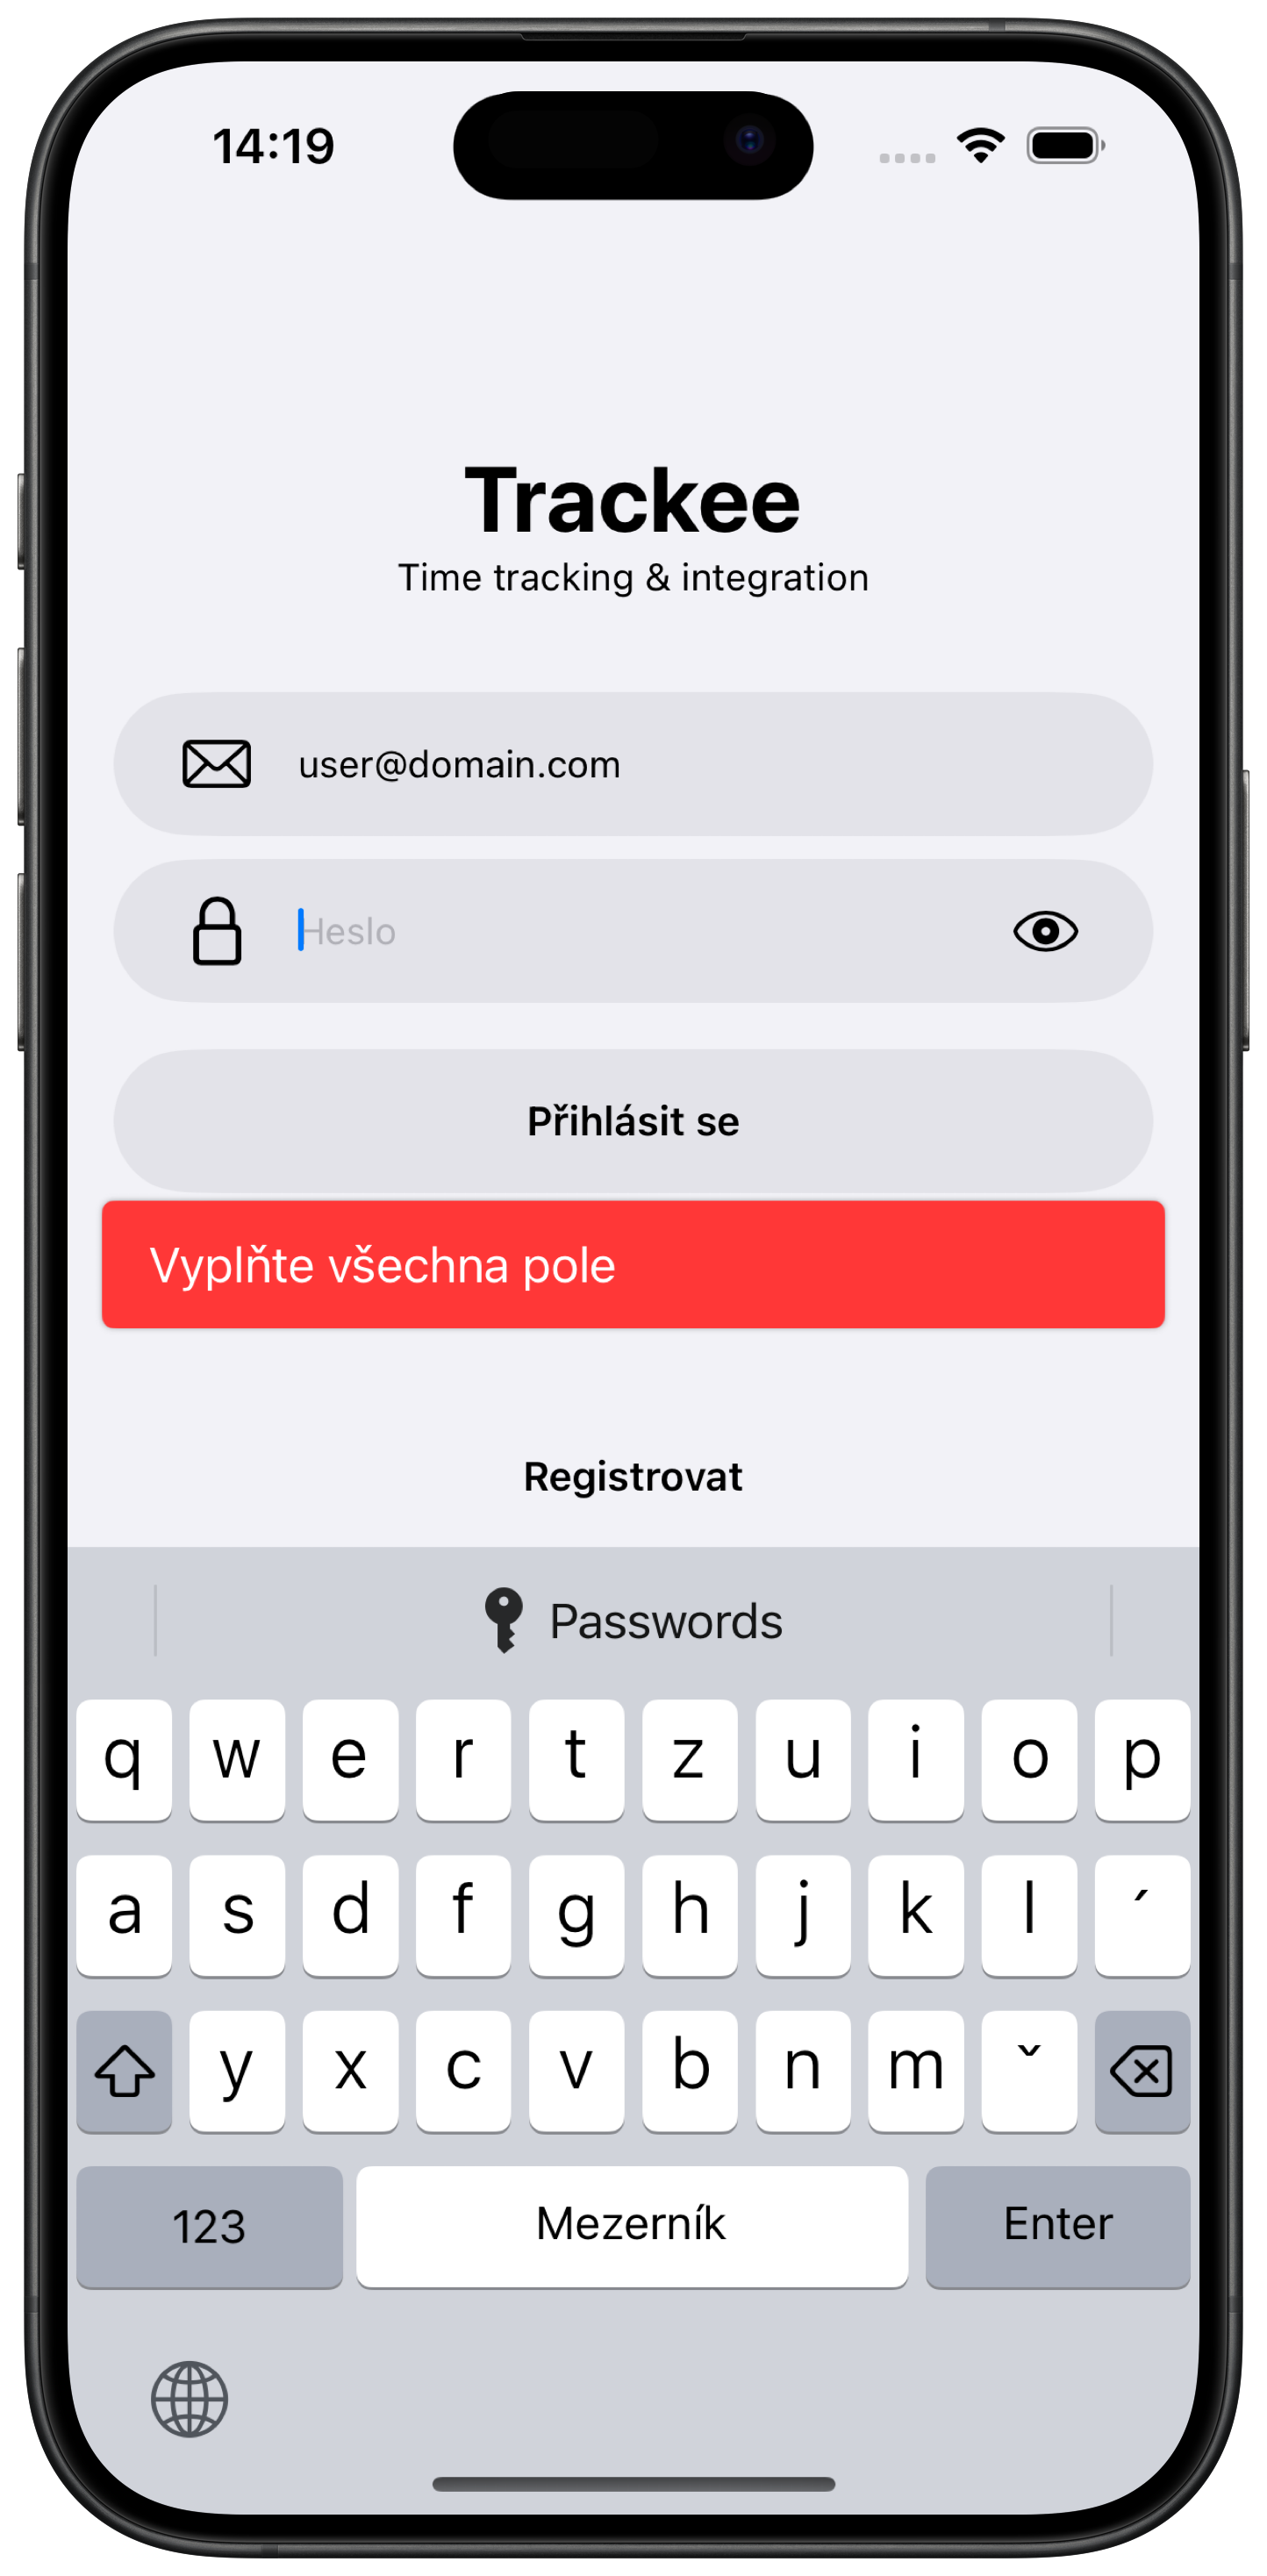
\includegraphics[width=6cm]{login-error-impl.png}
		\caption{Chyba při přihlášení}
		\label{fig:login-error-impl}
	\end{subfigure}
	\hspace{2cm}
	\begin{subfigure}[b]{0.4\textwidth}
		\centering
		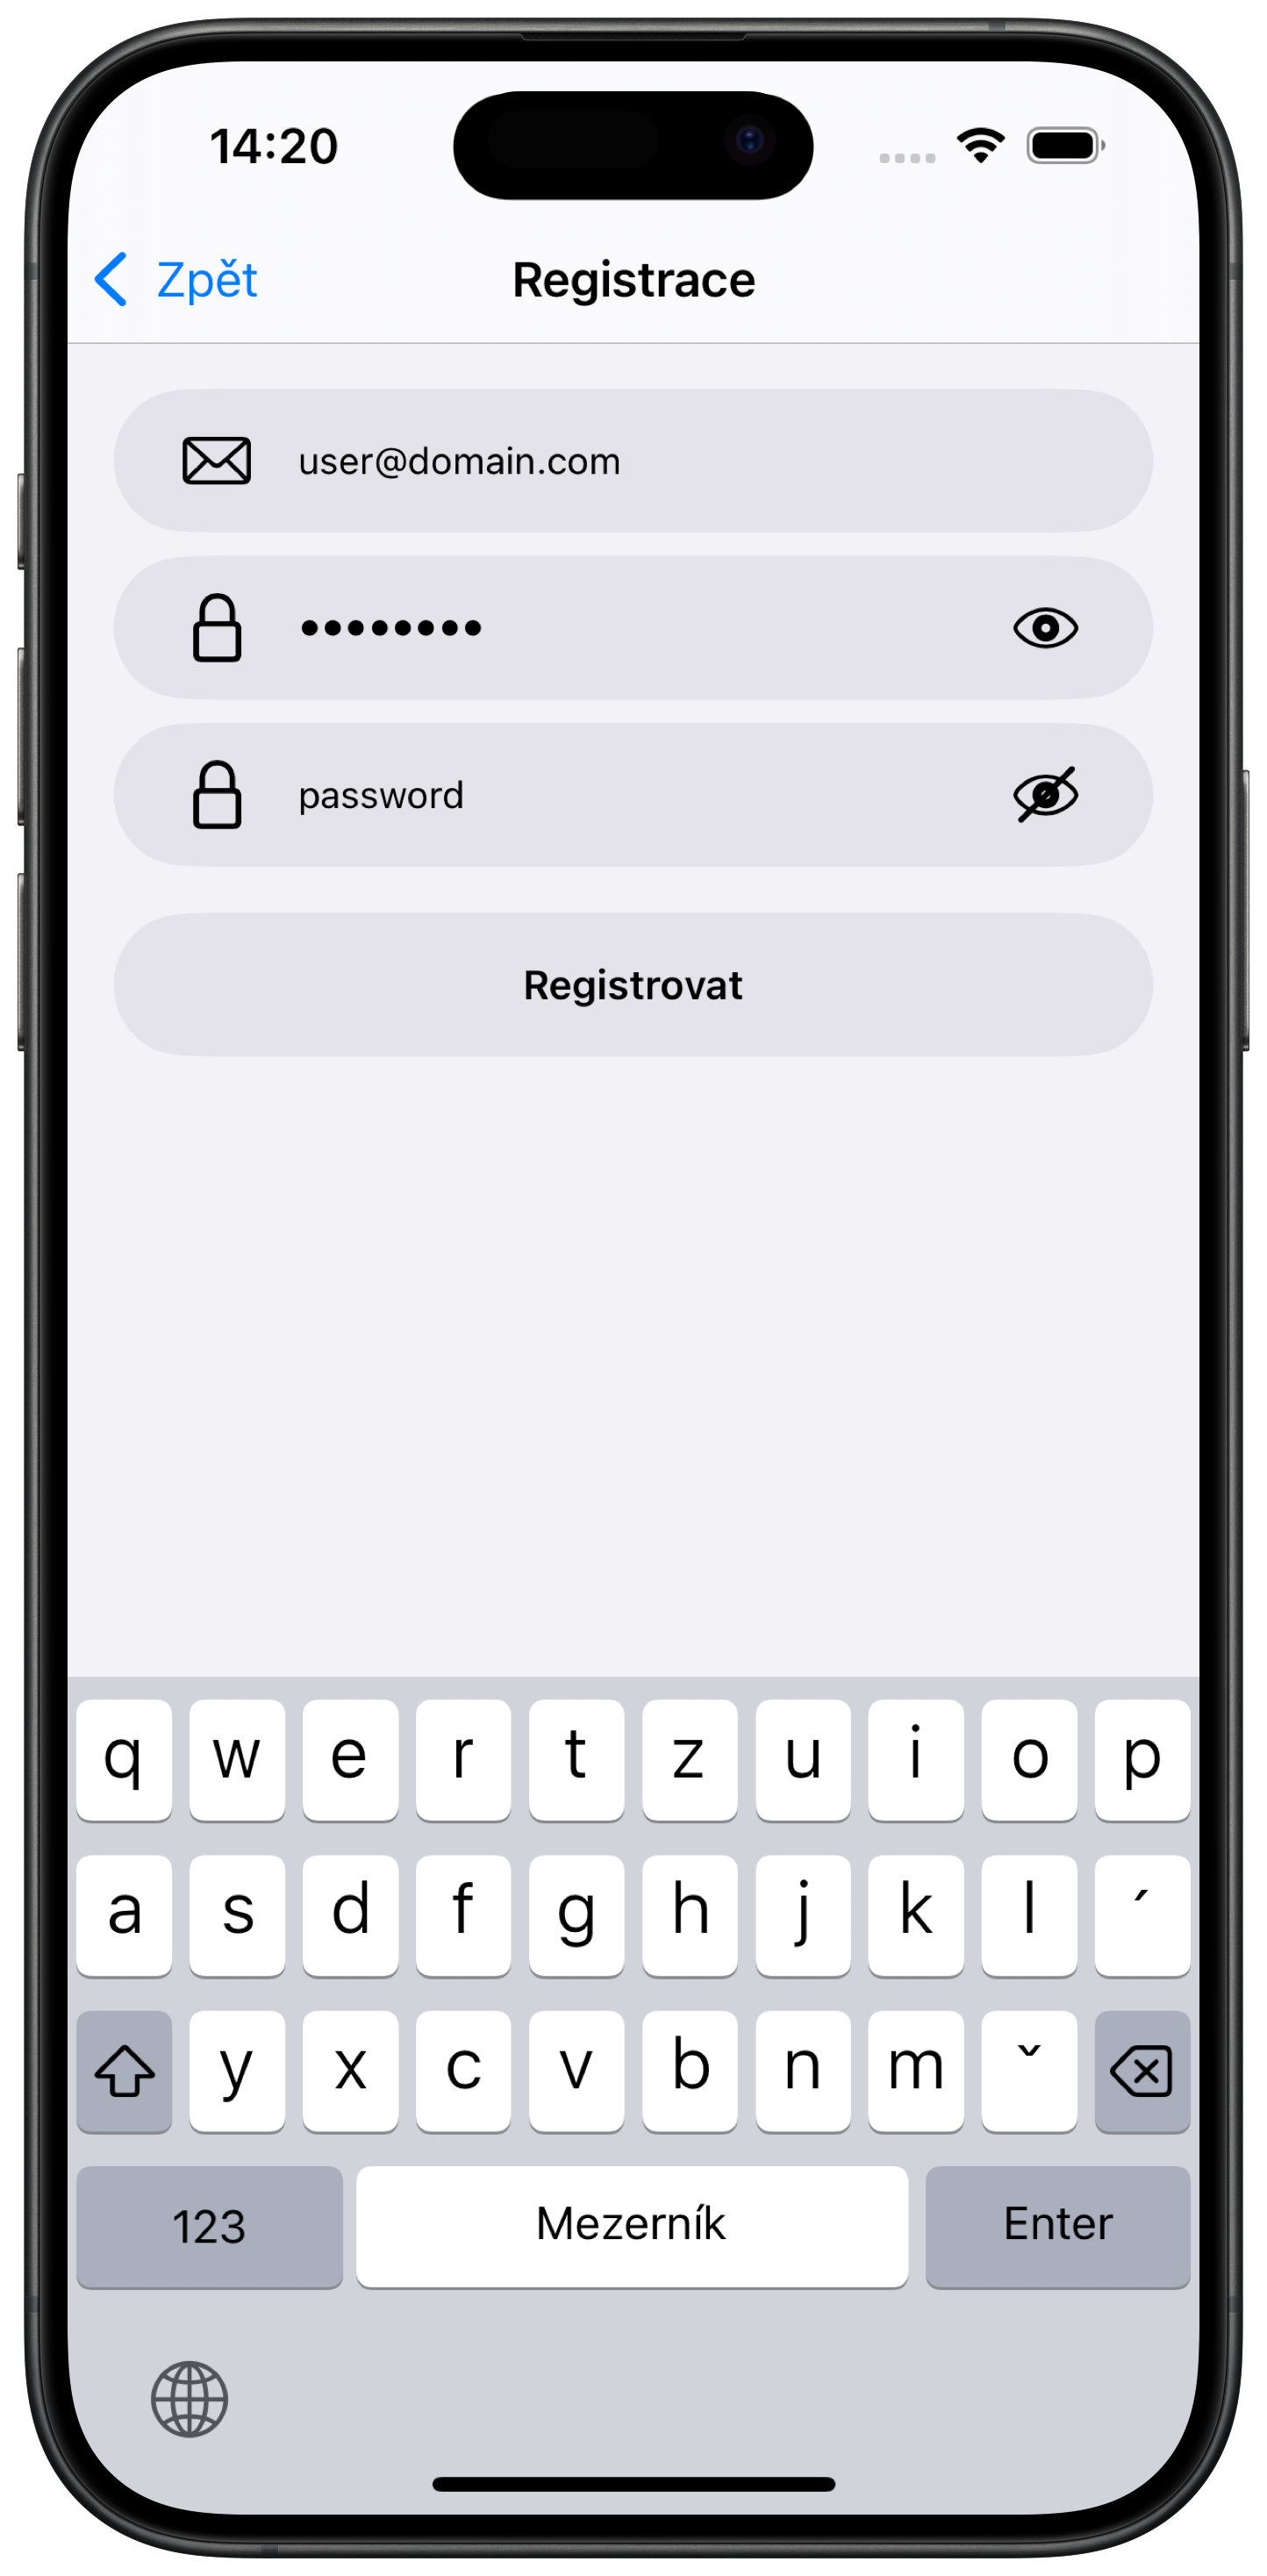
\includegraphics[width=6cm]{register-impl.png}
		\caption{Registrace}
	\end{subfigure}
	\caption{Realizace přihlášení a registrace}
	\label{fig:onboarding-impl}
\end{figure}

%---------------------------------------------------------------
\subsection{Časovač}
%---------------------------------------------------------------

Tato funkcionalita pokrývá veškeré operace s~ovládáním časovače, získáváním historie časových záznamů a vytváření nových záznamů. Jedná se o~hlavní funkci aplikace.

%---------------------------------------------------------------
\subsubsection{Backend}
%---------------------------------------------------------------

Backednová část platformy bude muset obsluhovat veškerá data, která se týkají časovače a časových záznamů. Backend je ale rozdělený podle funkcionalit jiným způsobem, než nativní aplikace a multi-platformní část, které jsou rozděleny podle funkcionalit z~hlediska uživatele. Moduly backendu jsou rozděleny podle toho, čeho se data v~modulu týkají, tedy například klienti, projekty, integrace a uživatel. Jelikož pro data časovače budou potřeba data uživatele, u~kterého se ukládá aktuální nastavení časovače a historie časových záznamů, ale také data projektů a klientů, bude implementace funkcionality časovače zasahovat do více modulů. Největší část funkcionality časovače bude obsluhovat modul uživatele. 

Obrazovka časovače bude potřebovat následující data – souhrn odpracovaných hodin v~aktuální den a týden, historii časových záznamů, aktuální nastavení časovače a přehled projektů, bude-li si uživatel chtít vybrat projekt, který časovači přidělí.

V~první řadě je tedy potřeba implementovat získávání historie časových záznamů, protože to bude potřeba i~pro výpočet odpracovaných hodin v~aktuálním dnu a týdnu. V~návrhu v~sekci \ref{feature-timer} bylo popsáno, že načítání historie časových záznamů by mělo podporovat stránkování, jelikož může teoreticky obsahovat velké množství záznamů, a pokud by se mělo velké množství načítat celé najednou, mohlo by to trvat dlouho a mohlo by se jednat o~velké množství dat, která by ale uživatel nejspíš ani všechna vůbec nepotřeboval. \texttt{UserRepository} tedy definuje mimo jiné funkce pro získávání záznamů, které lze nahlédnout v~ukázce kódu \ref{code:be-read-entries-interface}. Tyto funkce potřebují parametr \texttt{uid} identifikující uživatele, pro kterého mají být záznamy čteny, a dále přijímají nepovinné parametry pro specifikaci toho, od kdy a do kdy mají být záznamy čteny, a kolik maximálně záznamů se ve stránce má nacházet. Pokud bude mít některý z~těchto nepovinných parametrů hodnotu \texttt{null}, nebude žádné omezení na záznamy klást. Rozdíl mezi funkcemi, které vrací stránky objektu \texttt{TimerEntry} a stránky objektu \text{TimerEntryPreview} je ten, že objekt \texttt{TimerEntryPreview} obsahuje navíc celé zdrojové objekty klienta a projektu, který k~záznamu patří, zatímco \texttt{TimerEntry} obsahuje pouze jejich identifikátory. V~obrazovce pro zobrazení historie záznamů budou tyto zdrojové objekty potřebovat, protože při jejich vizualizaci (při jejich \emph{preview}) bude potřeba zobrazit jméno klienta a projektu.

\begin{listing}
\caption{Funkce pro získávání časových záznamů v~\texttt{UserRepository}}\label{code:be-read-entries-interface}
\begin{minted}{Kotlin}
interface UserRepository {

    // ...
    
    suspend fun readEntries(
        uid: String,
        startAfter: Instant?,
        limit: Int?,
        endAt: Instant?
    ): Page<TimerEntry>
    
    // ...
    
    suspend fun readEntryPreviews(
        uid: String,
        startAfter: Instant?,
        limit: Int?,
        endAt: Instant?
    ): Page<TimerEntryPreview>
    
    // ...
}
\end{minted}
\end{listing}

V~ukázce kódu \ref{code:be-read-entries-source} lze poté vidět, jakým způsobem aplikace získává záznamy přímo z~\emph{Firestore} databáze. Omezení ve smyslu od kdy do kdy záznamy číst a kolik maximálně jich přečíst se implementuje pomocí funkcí \texttt{startAfter(start)}, \texttt{endAt(end)} a \texttt{limit(limit)}, které přímo nabízí \emph{Firestore} API. \texttt{UserRepositoryImpl} používá tuto \emph{Source} funkci i~pro načtení \emph{preview} objektů, objekty klienta a projektu si pak pomocí identifikátoru načte sama a připojí je.

\begin{listing}
\caption{Funkce pro získávání časových záznamů v~\texttt{UserSourceImpl}}\label{code:be-read-entries-source}
\begin{minted}{Kotlin}
internal class UserSourceImpl : UserSource {

    // ...
    
    override suspend fun readEntries(
        uid: String,
        startAfter: Instant?,
        limit: Int?,
        endAt: Instant?
    ): Page<FirestoreTimerEntry> {
        val entriesCollection = db
            .collection(SourceConstants.Firestore.Collection.ENTRIES)
            .document(uid)
            .collection(SourceConstants.Firestore.Collection.ENTRIES)
            .orderBy(
                SourceConstants.Firestore.FieldName.STARTED_AT, 
                Query.Direction.DESCENDING
            )

        val snapshot = entriesCollection
            .startAfter(startAfter?.toTimestamp() ?: Timestamp.now())
            .endAt(endAt?.toTimestamp() ?: Timestamp.MIN_VALUE)
            .limit(limit ?: Int.MAX_VALUE)
            .get()
            .await()

        val data = snapshot.documents.map { it.toObject(FirestoreTimerEntry::class.java) }

        val remainingCount = entriesCollection
            .startAfter(data.lastOrNull()?.startedAt ?: Timestamp.MIN_VALUE)
            .count()
            .get()
            .await()
            .count

        return Page(
            data = data,
            isLast = remainingCount == 0.toLong()
        )
    }
    
    // ...
}
\end{minted}
\end{listing}

Při načítání historie záznamů na obrazovce časovače pak bude potřeba použít parametry \texttt{startAfter}, abychom definovali datum a čas, od kterého další záznamy načítat, pokud načítáme další stránky, a \texttt{limit}, který určí velikost stránky. Při načítání všech záznamů v~nějakém období se pak využije parametrů \texttt{startAfter} a \texttt{endAt}, například když bude potřeba zjistit souhrn odpracovaných hodin v~aktuální den nebo týden. Při výpočtu tohoto souhrnu bude tedy \texttt{UserRepositoryImpl} sčítat doby trvání všech záznamů v~daném období.

Pro obsluhu časovače pak \texttt{UserRepository} poskytuje funkce pro načtení dat časovače a pro jejich aktualizaci. Při výběru projektu bude uživatel potřebovat vidět všechny své projekty a názvy jejich klientu, pro což bude sloužit opět \emph{preview} objekt \texttt{ProjectPreview}. \texttt{ClientRepository} tedy nabízí funkce pro získání klienta podle identifikátoru, a \texttt{UserRepository} nabízí funkce pro získání projektu podle identifikátoru klienta a projektu, ale také funkci pro získání všech projektů daného uživatele.

Pro komunikaci s~klientem se také využívá vlastních struktur pro reprezentaci chyb. Například modul \texttt{user} používá výjimky ze skupiny \texttt{UserExceptions}, která dědí z~třídy \texttt{BaseException}. V~případě, že některé volání vrátí výjimku s~tímto rodičem, tak ji komunikace umí zakódovat do DTO reprezentace, která je známá pro klienta. Ten může potom rozlišovat mezi různými známými chybami. V~případě, že se nejedná o~známou chybu, zakóduje ji komunikace jako obecnou chybu s~HTTP status kódem 500. Implementace tohoto chování lze nahlédnout ve výpisu kódu \ref{code:be-error-handling}.

\begin{listing}
\caption{Obsluha chyb na backendu}\label{code:be-error-handling}
\begin{minted}{Kotlin}
fun Application.configureRouting(isDebug: Boolean) {
    install(StatusPages) {
        exception<BaseException> { call, baseException ->
            call.respond(
                status = baseException.code,
                message = baseException.toDto(isDebug)
            )
        }

        exception<Throwable> { call, cause ->
            call.respond(
                status = HttpStatusCode.InternalServerError,
                message = ErrorDto(
                    type = "InternalError",
                    message = "Internal Server Error",
                    debugMessage = if (isDebug) cause.message else null
                )
            )
        }
    }
    
    // ...
}
\end{minted}
\end{listing}

%---------------------------------------------------------------
\subsubsection{Multi-platformní část}
%---------------------------------------------------------------

Multi-platformní část aplikace už rozděluje své moduly podle funkcionalit z~hlediska uživatele, modul \texttt{timer} bude tedy poskytovat všechny \emph{Use Cases} pro potřeby časovače:
\begin{itemize}
\item\texttt{AddTimerEntryUseCase} – Vytvoří nový časový záznam podle parametrů.
\item\texttt{DeleteTimerEntryUseCase} – Smaže časový záznam podle identifikátoru.
\item\texttt{GetProjectsUseCase} – Získá \emph{preview} objekty všech projektů, které má uživatel přiřazeny.
\item\texttt{GetTimerDataPreviewUseCase} – Získá \emph{preview} objekt pro aktuální nastavení časovače. Čistá data o~aktuálním stavu časovače totiž opět obsahují jen identifikátory klienta a projektu, ale při vizualizaci dat jsou potřeba jejich názvy.
\item\texttt{GetTimerEntriesUseCase} – Získává stránky \emph{preview} objektů časových záznamů, umí tedy pracovat se všemi parametry pro omezení stránky. Zároveň časové záznamy seskupuje do seznamu objektů typu \texttt{TimerEntryGroup}, což je skupina, která obsahuje datum, seznam všech záznamů patřící k~tomuto datu a součet odpracovaných hodin všech těchto záznamů. Toho se využije při vizualizaci v~nativní aplikaci, kde se nad každou skupinou ukáže datum a časový souhrn pro daný den.
\item\texttt{GetTimerSummariesUseCase} – Získá souhrny časových záznamů pro aktuální den a týden.
\item\texttt{UpdateTimerDataUseCase} – Aktualizuje aktuální nastavení časovače.
\end{itemize}

Všechny tyto \emph{Use Cases} automaticky počítají s~tím, že pracují s~daty aktuálně přihlášeného uživatele, žádné parametry pro jeho identifikaci tedy nepotřebují.

Jednotlivé \emph{Use Cases} už komunikují s~backendem, a to v~nejnižší \emph{infrastructure} vrstvě, která požadavky posílá pomocí knihovny \emph{Ktor}. Příklad toho, jak probíhá komunikace, lze nahlédnout v~ukázce kódu \ref{code:kmp-read-entries-source-impl}.

\begin{listing}
\caption{Funkce pro získávání časových záznamů v~\texttt{RemoteTimerSource}}\label{code:kmp-read-entries-source-impl}
\begin{minted}{Kotlin}
internal class RemoteTimerSource(
    private val client: HttpClient
) : TimerSource {
    override suspend fun readEntries(
        startAfter: String?,
        limit: Int?,
        endAt: String?
    ): Result<PageDto<TimerEntryDto>> =
        runCatchingCommonNetworkExceptions {
            val res = client.get("user/entries") {
                url {
                    startAfter?.let { parameters.append("startAfter", it) }
                    limit?.let { parameters.append("limit", it.toString()) }
                    endAt?.let { parameters.append("endAt", it) }
                }
            }
            res.body<PageDto<TimerEntryDto>>()
        }
        
    // ...
}
\end{minted}
\end{listing}

Multi-platformní část pracuje s~objekty v~DTO reprezentaci, kterou definuje backend. Poté si je také převádí pomocí vlastních funkcí do vlastních doménových reprezentací.

Také lze ve výpisu kódu \ref{code:kmp-read-entries-source-impl} nahlédnout, že celé API volání je obaleno do pomocné funkce \texttt{runCatchingCommonNetworkExceptions}, jejíž implementace lze nahlédnout ve výpisu \ref{code:kmp-run-catching-common-network-exceptions}. Tato funkce odchytává všechny výjimky, které při komunikaci s~backendem mohou vzniknout, a převádí je do vlastních reprezentací, se kterými poté umí pracovat nativní aplikace.

\begin{listing}
\caption{Odchytávání výjimek při komunikaci s~backendem}\label{code:kmp-run-catching-common-network-exceptions}
\begin{minted}{Kotlin}
internal suspend inline fun <R : Any> runCatchingCommonNetworkExceptions(
    block: () -> R
): Result<R> =
    try {
        Result.Success(block())
    } catch (e: ResponseException) {
        val body = e.response.body<ErrorDto>()

        when (body.type) {
            "Unauthorized" -> Result.Error(
                BackendError.NotAuthorized(e.response.toString(), e),
            )

            "ProjectNotAssignedToUser" -> Result.Error(
                BackendError.ProjectNotAssignedToUser(e.message, e)
            )

            "MissingProject" -> Result.Error(
                BackendError.MissingProject(e.message, e)
            )

            "ProjectNotFound" -> Result.Error(
                BackendError.ProjectNotFound(e.message, e)
            )

            "ClientNotFound" -> Result.Error(
                BackendError.ClientNotFound(e.message, e)
            )

            else -> Result.Error(
                ErrorResult(
                    message = body.message,
                    throwable = e
                )
            )
        }
    } catch (e: Throwable) {
        Result.Error(handlePlatformError(e))
    }
\end{minted}
\end{listing}

%---------------------------------------------------------------
\subsubsection{Nativní aplikace}
%---------------------------------------------------------------

%---------------------------------------------------------------
\subsection{Profil uživatele}
%---------------------------------------------------------------

%---------------------------------------------------------------
\subsubsection{Nativní aplikace}
%---------------------------------------------------------------

%---------------------------------------------------------------
\subsubsection{Multi-platformní část}
%---------------------------------------------------------------

%---------------------------------------------------------------
\subsubsection{Backend}
%---------------------------------------------------------------

%---------------------------------------------------------------
\subsection{Integrace}
%---------------------------------------------------------------

%---------------------------------------------------------------
\subsubsection{Nativní aplikace}
%---------------------------------------------------------------

%---------------------------------------------------------------
\subsubsection{Multi-platformní část}
%---------------------------------------------------------------

%---------------------------------------------------------------
\subsubsection{Backend}
%---------------------------------------------------------------


%---------------------------------------------------------------
\chapter{Testování}
%---------------------------------------------------------------

Výslednou aplikaci a její uživatelské rozhraní je potřeba důkladně otestovat. Tato kapitola popisuje implementaci automatických testů a scénáře testování s~reálnými uživateli. Výsledky z~testování jsou poté zhodnoceny.

%---------------------------------------------------------------
\section{Automatické testování}
%---------------------------------------------------------------

Pro účely automatizovaného testování se u~Apple platforem používá knihovna \emph{XCTest} \cite{xctest}. Jak již bylo zmíněno, \emph{Clean architecture} ja navržená tak, aby se dala dobře otestovat jednotkovými testy, které jsou popsány v~následující sekci.

Dalšími možnostmi testování jsou UI testy a testy výkonu. Aplikace Trackee implementaci těchto typů testů neobsahuje. Jejich implementace může být podnětem pro budoucí vylepšení aplikace.

%---------------------------------------------------------------
\subsection{Jednotkové testování}
%---------------------------------------------------------------

V~aplikaci jsou jednotkovými testy pokryty všechny \emph{View Modely}. Pro každý z~nich je v~modulu, ke kterému patří, soubor, který daný \emph{View Model} testuje. Např. pro \texttt{LoginViewModel.swift} bude testovací soubor \texttt{LoginViewModelTests.swift}.

\emph{View Model} testy jsou navržené tak, aby testovaly každý jednotlivý \emph{Intent}, pokud existuje vhodná možnost, jak test provést. Některé intenty vhodně otestovat nelze – například takové, které otevírají nějaké systémové dialogy, které nemají žádný výstup pro \emph{View Model} aplikace. Daný test tedy vždy ověřuje, zda se stav \emph{View Modelu} po aplikování \emph{Intentu} změnil podle očekávání.

Jednotkové testy \emph{View Modelů} využívají \emph{Mocky} pro \emph{Use Cases}, tedy určité zjednodušené náhrady těchto \emph{Use Cases}, u~kterých si každý test může definovat, co bude daný \emph{Use Case Mock} vracet za hodnotu. Toto je klasický přístup k~jednotkovému testování – testujeme zde \emph{View Modely}, nikoli \emph{Use Cases}.

Předpokládejme tedy, že máme \emph{View Model} se strukturou ve výpisu \ref{code:tested-vm-structure}. Struktura testu poté bude vypadat jako ve výpisu \ref{code:vm-test-sctructure}. Struktura obsahuje následující:
\begin{itemize}
\item\texttt{flowController} – \emph{Mock} pro \emph{FlowController}, tedy náhrada reálného controlleru v aplikaci. Tento \emph{Mock} slouží k~tomu, abychom mohli otestovat, jaká hodnota byla vložena do posledního volání funkce \texttt{handleFlow(\_:)} a kolikrát byla tato funkce zavolána. Toto slouží k~otestování toho, zda se bude apikace snažit uživatele navigovat do předpokládané destinace.
\item\emph{Mocky} pro \emph{Use Cases} – zde vytváříme instance \emph{Mocků} pro \emph{Use Cases}, které jsou v~daném \emph{View Modelu} používány. Je potřeba to dělat takto ručně, protože kdybychom použili registrování pomocí \texttt{Container.shared.registerUseCaseMocks()}, tak bychom nemohli v~testech měnit hodnoty, které dané \emph{Use Cases} budou vracet.
\item\texttt{createViewModel()} – tato funkce se bude volat na začátku každého testu, aby získal instanci pro otestování. Pokud konstruktor \emph{View Modelu} vyžaduje nějaké parametry, můžou být předány jako parametr této funkce, nebo zde můžou mít nějakou definovanou hodnotu. V~této funkci se také registrují \emph{Mocky} pro \emph{Use Cases} definované výše.
\item Testovací funkce pro jednotlivé intenty – funkce, které mají v~názvu prefix \texttt{test}, tak se automaticky považují ze testovací funkce a spouštějí se během testu. Každý vhodně otestovatelný intent zde tedy bude mít vlastní funkci, případně více funkcí, pokud lze otestovat úspěch, neúspěch, různé formy úspěchu, a podobně. Tyto funkce dodržují strukturu given-when-then, tedy rozdělení do tří částí (předdefinované hodnoty a konstanty, interakce, ověření).
\end{itemize}

\begin{listing}
\caption{Struktura View Modelu pro testování}\label{code:tested-vm-structure}
\begin{minted}{Swift}
final class SomeViewModel: BaseViewModel, ViewModel, ObservableObject {
	
    // ...
	
    @Injected(\.someUseCase) private var someUseCase
	
    // ...
	
    enum Intent {
        case doThis
        case doThat
    }
	
    // ...
}
\end{minted}
\end{listing}

\begin{listing}
\caption{Struktura View Model testu}\label{code:vm-test-sctructure}
\begin{minted}{Swift}
@MainActor
final class SomeViewModelTests: XCTestCase {

    private let flowController = FlowControllerMock<SomeFlow>(
        navigationController: UINavigationController()
    )
    
    private let someUseCaseMock = SomeUseCaseMock(
        executeReturnValue: /* Some default return value */
    )
    
    private func createViewModel(
        someOptionalParam: SomeType
    ) -> SomeViewModel {
        Container.shared.someUseCase.register { self.someUseCaseMock }
	
        return SomeViewModel(
            someParam: someOptionalParam,
            flowController: flowController
        )
    }
    
    // MARK: - Tests
    
    func testDoThis() async {
        // given
        let vm = createViewModel()
        // ... some constants and given values
        let someConstant = ...
    	
        // when
        vm.onIntent(.doThis)
        // ... some interactions
        await vm.awaitAllTasks()
		
        // then
        // ... assertions
        XCTAssertEqual(vm.state.someValue, someConstant)
    }
    
    func testDoThat() async {
        // ...
    }
}
\end{minted}
\end{listing}

Jednotkové testy \emph{View Modelů} testují byznysovou prezentační vrstvy. Pro otestování dalších vrstev je možné v multiplatformním modulu testovat \emph{Use Cases}, \emph{Repositories} a \emph{Sources}. V backendové části je také možné implementovat jednotkové testy pro \emph{Repositories}, \emph{Sources}, ale i~pro \emph{Routes}. Implementace testů pro tyto vrstvy může být podnětem pro budoucí vylepšení aplikace.

%---------------------------------------------------------------
\section{Uživatelské testování}
%---------------------------------------------------------------

Pro účely uživatelského testování byl navržen scénář, podle kterého se testeři mají řídit. Proces testování je rozdělen do několika scénářů, které by měly pokrývat většinu funkcionalit aplikace, kterých uživatel může využít. Povinnými účastníky během testování budou moderátor a uživatel. Moderátor bude uživateli dávat instrukce a dokumentovat, jak uživatel s~mobilním telefonem interaguje. Uživatel se bude snažit instrukce plnit a bude při tom nahlas popisovat své akce s~telefonem (co vidí, na co se chystá kliknout, co očekává, že se stane, atd.), aby usnadnil následnou analýzu celé situace. 

Uživatelského testování se zúčastnilo 5 testerů. Záznamy z~testování lze nahlédnout v~\cite{ui-testing-playlist}. Přehled testerů lze nahlédnout v~tabulce \ref{table:testers}. Instrukce, podle kterých se testeři řídili, lze nahlédnout v~příloze \ref{appendix:ui-testing-instructions}. Protokol z~testování lze nahlédnout v~příloze \ref{appendix:ui-testing-protocol}.

\begin{table}\centering
\begin{tabular}{l|c|c|c}
	Tester		& Pohlaví	& Používaný OS	& Používá aplikace pro měření času	\tabularnewline \hline 
 	F. W.		& Muž		& Android       & ANO (Clockify)	                \tabularnewline \hline
	D. K.		& Muž		& iOS	        & ANO (Clockify)                	\tabularnewline \hline
	D. Ž.		& Muž		& Android       & ANO (Clockify)               		\tabularnewline \hline
	E. Č.		& Žena		& iOS	        & NE 	                	        \tabularnewline \hline
	T. S.		& Muž		& Android       & ANO (Clockify)	                \tabularnewline \hline
\end{tabular}
\vspace{0.5cm}
\caption[Přehled testerů aplikace]{~Přehled testerů aplikace}\label{table:testers}
\end{table} 

%---------------------------------------------------------------
\subsection{Scénář}
%---------------------------------------------------------------

\begin{description}
\item[Tvorba uživatelského účtu:] Každý nový uživatel mobilní aplikace Trackee si bude muset nejprve vytvořit svůj uživatelský účet. V~tomto scénáři bude uživatel instruován k~tomu, aby aplikaci poprvé spustil, vytvořil si nový uživatelský účet pomocí předepsaného e-mailu a hesla a následně se do aplikace pod tímto účtem přihlásil. 
\item[Vytvoření nového klienta:] Po úspěšné registraci bude uživatel instruován, aby si vytvořil 2 nové klienty s~předepsanými názvy.
\item[Vytvoření nového projektu:] Po úspěšném vytvoření klientů bude uživatel instruován, aby vytvořil 2 nové projekty s~předepsanými vlastnostmi.
\item[Spuštění časovače:] Po úspěšném vytvoření projektů dostane uživatel instrukci, aby spustil časovač pro měření odpracovaného času a přiřadil mu předepsaný projekt a popis.
\item[Změna začátku časovače:] Uživatel bude instruován k~tomu, aby u~spuštěného časovače změnil začátek na předepsaný čas.
\item[Zastavení časovače:] Uživatel bude instruován, aby ukončil časovač a uložil časový záznam, který do teď měřil.
\item[Manuální přidání časového záznamu:] Uživatel bude instruován, aby ručně přidal časový záznam s~předepsanými parametry a časem.
\item[Úprava projektu:] Uživatel bude instruován, aby aktualizoval předepsaný projekt s~novými předepsanými vlastnostmi.
\item[Odhlášení a přihlášení na testovací účet:] Uživatel ve svém nově vytvořeném účtě nebude mít dostatek klientů, projektů a časových záznamů, které by odpovídaly dlouhodbějšímu používání aplikace. Pro lepší otestování orientace v~aplikaci bude uživatel instruován, aby se přihlásil na předepsaný testovací účet, který obsahuje větší množství záznamů.
\item[Odstranění časového záznamu:] Uživatel bude instruován, aby odstranil předepsaný časový záznam z~historie.
\item[Export historie do CSV souboru:] Uživatel bude instruován, aby vytvořil integraci pro exportování do CSV souboru a exportoval data do tabulky pro předepsané časové období. Dále bude instruován, aby tuto tabulku otevřel ve vhodné aplikaci, kde si ji může prohlédnout (např. \emph{Numbers}).
\item[Odstranění klienta:] Budeme předpokládat, že si uživatel v~exportované tabulce všimne, že tam má záznamy patřící předepsanému klientovi, které tam mít nechce. Bude tedy instruován, aby klienta smazal a znovu vyexportoval CSV soubor, ve kterém zkontroluje, že žádné záznamy patřící k~tomuto klientovi nejsou.
\item[Tvorba automatizace pro spuštění časovače:] Uživatel dostane instrukci, aby pomocí aplikace \emph{Zkratky} vytvořil novou automatizaci, která zapne časovač s~předepsanými parametry, pokud se uživatel objeví na předepsané poloze. Bude také instruován, aby tuto automatizaci zkusil ručně spustit a v~aplikaci zkontroloval, že časovač opravu běží.
\item[Tvorba automatizace pro vypnutí časovače (odstraněno):] Uživatel bude požádán, aby vytvořil automatizaci, která se ho zeptá, zda nechce zastavit běžící časovač, pokud opustí předepsanou polohu. Zde bude také instruován, aby automatizaci zkusil ručně spustit. Tento scénář byl po několika testech ze seznamu odstraněn, protože bylo zhodnoceno, že je příliš podobný předchozímu scénáři a zároveň přímo netestuje rozhraní samotné aplikace.
\end{description}


%---------------------------------------------------------------
\chapter{Prostředí pro budoucí podporu a~provoz aplikace}
%---------------------------------------------------------------

Během tvorby této práce vzniklo mnoho podnětů pro budoucí vývoj a vylepšení aplikace. Už v~samotném návrhu nebo realizaci byla rozebírána řada možností, které v~této práci realizovány nejsou, ale bylo by je vhodné v~budoucnu implementovat. Během uživatelského testování pak vznikla řada doporučení pro úpravu rozhraní aplikace.

%---------------------------------------------------------------
\section{Zrychlení komunikace a lokální data}
%---------------------------------------------------------------

Prvním tématem, kterému by se budoucí provoz aplikace měl zabývat, je celkové zrychlení manipulace s~aplikací. Jsou dvě zásadní věci, které zpomalují interakci s~aplikací a které vyžadují vylepšení.

%---------------------------------------------------------------
\subsection{Komunikace s~databází}
%---------------------------------------------------------------

Pomalá komunikace s~databází je způsobena hlavně tím, že zvolená řešení pro nasazení backendu a databáze provozují jejich instance navzájem vzdálené 8 000 km od sebe. Důvody, proč tomu tak je, byly popsány v~sekci \ref{development-tools}. Nejlepším řešením tohoto problému by bylo používat takové nástroje, které minimalizují vzdálenost mezi backendem a databází, která ale budou pravděpodobně vyžadovat placené plány. Mezi backendem a databází ale probíhá největší počet požadavků na čtení či zápis, jejich vzájemná komunikace je proto ještě důležitější, než komunikace mezi backendem a samotným klientem.

%---------------------------------------------------------------
\subsection{Lokálních data (cache)}
%---------------------------------------------------------------

Moderní aplikace obvykle využívají nějakou formu lokální \emph{cache}, která může mít mnoho využití, jako například dočasné zastoupení vzdálených dat z~databáze. Vhodné navržení a implementace takové \emph{cache} je ale poměrně komplexní záležitost a proto nemohla být realizována v~rámci této práce. Lokální \emph{cache} by šlo využít mimo jiné takto:
\begin{itemize}
\item{\emph{UseCases}, které vrací různé seznamy dat (záznamy, klienty, projekty, \dots), by místo prostého vrácení jedné hodnoty mohly vracet nějaký \emph{stream} dat (napříkad \emph{KotlinX Flow} \cite{kotlinx-flow}), které by nejprve vrátily data z~\emph{cache} lokální databáze, a hned jak by přišly data ze vzdálené databáze, tak by se data nahradily těmito daty a také by byla aktualizována \emph{cache}. Tímto způsobem by v~podstatě zmizely prodlevy, ve kterých musí uživatel čekat, než se mu zobrazí data a může interagovat s~aplikací. Je však potřeba v~jednotlivých případech počítat s~tím, kdy aplikace nějaká data aktualizuje – tehdy je potřeba na vzdálená data počkat.}
\item{Funkcionality, které nějakým způsobem aktualizují data (ovládání časovače, uložení záznamu, tvorba/úprava klienta nebo projektu, \dots), by nemusely po aplikování změn čekat na to, až aktualizovaná data přijdou, ale mohly by rovnou zobrazit data v~takovém formátu, v~jakém by aplikace předpokládala, že aktualizovaná data budou vypadat (například při vytvoření klienta se klient rovnou zobrazí v~seznamu klientů a až po chvíli jeho přidání potvrdí vzdálená data). Bylo by však třeba v~případě, že aktualizace dat selže, vrátit data do původního stavu, před očekávanou aktualizací.}
\end{itemize}

Implementace aplikace je pro využití lokální \emph{cache} dobře připravena. V~multi-platformní části již obsahuje nástroje pro manipulaci s~lokální databází pomocí knihovny \emph{SQLDelight} \cite{sqldelight}. Lze také v~implementaci nahlédnout, že v~multi-platformní části se jednotlivé \emph{sources} jmenují například \texttt{RemoteIntegrationSource}, což představuje zdroj vzdálených dat (z~backendu) pro integraci. Při použití lokální databáze by se definoval \texttt{LocalIntegrationSource}, který by implementoval obdobné funkcionality, a logika toho, kdy a jak se má který typ \emph{source} použít, by byla obsažena v~konkrétní \emph{repository}, v~uvedeném příkladě \texttt{IntegrationRepository}.

%---------------------------------------------------------------
\section{Úpravy uživatelského rozhraní}
%---------------------------------------------------------------

Z~průběhu uživatelského testování vzešla řada poznatků, ať už velmi důležitých nebo méně důležitých, které poukázaly na nějaké nedostatky či možnosti vylepšení v~uživatelském rozhraní aplikace. Důkladný popis, analýza a doporučení pro další vývoj aplikace, vycházejících z~těchto poznatků, je v~sekci \ref{ui-testing-results}, která by měla sloužit jako podnět budoucího vývoje.

%---------------------------------------------------------------
\section{Rozšíření funkcionalit}
%---------------------------------------------------------------

Funkcionality, které aplikace implementuje, mají také široký potenciál, jak rozšířit jejich možnosti a přinést tak uživatelům další funkce při používání aplikace. Mezi tyto možnosti může patřit:
\begin{itemize}
\item\textbf{Možnost úpravy časového záznamu.} Tato funkce by uživatelům ulehčila práci se záznamy, pokud například špatně zadají nějaké parametry záznamu. Také se jednalo o~jeden z~poznatků uživatelského testování – zájem ze strany uživatelů o~tuto funkci tedy určitě je.
\item\textbf{Více parametrů pro klienty.} U~klientů lze v~realizované aplikaci zadávat pouze název, pro různé budoucí účely se ale mohou hodit další parametry, jako třeba fakturační adresa klienta, různé poznámky, nebo barevné rozlišení.
\item\textbf{Více parametrů pro projekty.} U~projektů se také v~budoucnu mohou hodit další parametry, než ty, které aplikace v~tuto chvíli nabízí. Mezi ty může například patřit cena práce za hodinu u~konkrétního projektu, kterou lze využít během fakturace, nebo možnost vytvořit si vlastní typy projektů. 
\item\textbf{Reporty a shrnutí.} Mnoho existujících řešení pro měření a správu odpracovaného času umožňuje vytvářet nějaké formy reportů nebo vizualizací odpracovaného času. Uživatelé si mohou prohlížet, kolik práce vykonali v~určitých obdobích u~různých klientů a projektů, a podobně. Aplikace tuto funkci v~současné chvíli nemá a tvorbu takových shrnutí umožňuje pouze pomocí jiných nástrojů, například z~CSV dat, která aplikace poskytne.
\item\textbf{Integrace s~dalšími existujícími systémy.} V~analýze v~sekci \ref{existing-tracking-solutions} byly popsány různé existující systémy pro měření a správu odpracovaného času, spolu s~možnostmi integrace s~nimi. Realizace aplikace implementuje základ pro tyto integrace (CSV, \emph{Clockify}), ale potenciál těchto integrací je mnohem větší. Předmětem dalšího vývoje by tedy mohla být nějaká analýza toho, jaké další integrace by bylo vhodné implementovat a tyto integrace poté realizovat.
\item\textbf{Integrace s~hardwarovými spouštěči.} V~analýze byly také popsány možnosti hardwarových spouštěčů (fyzické ovladače apod.), které by šly využít při integraci s~aplikací. Pro propojení s~jedním z~nich by bylo potřeba implementovat BLE komunikaci. Zvážení této funkce také může být předmětem dalšího vývoje.
\item\textbf{Přihlášení přes externí poskytovatele.} \emph{Firebase} autentizace, které aplikace využívá, nabízí možnosti přihlášení přes \emph{Apple}, \emph{Facebook} a \emph{Google}. V~aplikaci je dokonce připraven \emph{provider} pro přihlášení přes \emph{Apple} – \texttt{AppleSignInProvider}.
\end{itemize}

%---------------------------------------------------------------
\section{Nasazení mezi reálné uživatele}
%---------------------------------------------------------------

V~realizaci v~sekci \ref{testflight} bylo popsáno, jakým způsobem byla aplikace nasazována pro účely testování během vývoje. Podobným způsobem se poté realizuje i~nasazení mezi reálné uživatele v~obchodě \emph{App Store}. Pro nahrání aplikace do tohoto obchodu také slouží nástroj \emph{App Store Connect}.

Jak již bylo také zmíněno, aplikace musí před schválením pro nasazení do obchodu \emph{App Store} projít procesem \emph{App Review}, ve kterém \emph{Apple} kontroluje splnění všech pravidel pro aplikace, které do obchodu míří. Aplikace už ale tímto procesem úspěšně prošla už v~rámci veřejného testování. \emph{App Review} pro \emph{App Store} je sice o~něco pečlivější než pro veřejné testování, ale zásadní porušení pravidel pro šíření aplikací v~\emph{App Store} by mělo být odhaleno již v~tomto procesu.

Ostatní nástroje, které jsou aplikací využívány, pak žádnou další konfiguraci pro nasazení mezi reálné uživatele nepotřebují. Backend i~databáze jsou nasazeny pod veřejně přístupnými doménami a aplikace je na ně napojena. Bude pouze potřeba monitorovat využití backendu nebo databáze, které jsou sice prozatím pod neplacenými plány, ale v~budoucnu budou pravděpodobně zapotřebí placené plány. Také bude podle využití potřeba zhodnotit, zda se stále vyplatí využívat funkce pro uspávání backendu, kterou \emph{Railway} nabízí.

%---------------------------------------------------------------
\section{Podpora pro další platformy}
%---------------------------------------------------------------

Návrh architektury platformy (sekce \ref{platform-architecture}) počítal s~možnostmi budoucího rozšíření podpory pro další platformy, jako je Android aplikace, webová aplikace a další. Toto rozšíření může být implementováno s~pomocí technologie \emph{Kotlin Multiplatform}, kterou klientská aplikace používá. Stačí přidat moduly pro nové platformy a jejich aplikace implementovat podobným stylem, jako nativní iOS aplikaci. Detailnější popis struktury celého projektu v~rámci \emph{monorepa} je v~realizaci v~sekci \ref{project-structure}.








































%---------------------------------------------------------------
\chapter*{Závěr}
%---------------------------------------------------------------
\addcontentsline{toc}{chapter}{Závěr}
\markboth{Závěr}{Závěr}

Hlavním cílem práce bylo analyzovat, navrhnout a~implementovat mobilní aplikaci pro systém iOS (frontend i~backend) pro zaznamenávání odpracovaného času, která měla umožnit integraci s~různými spouštěči akcí a~propojení s~dalšími systémy pro zaznamenávání a~spravování odpracovaného času. V~rámci návrhu bylo cílem navrhnout vhodné technické řešení pro implementaci aplikace, funkcionality aplikace a~jejich uživatelské rozhraní a~tohoto návrhu se poté při realizaci aplikace držet. Následně bylo cílem práce realizované řešení vhodně otestovat a~provést uživatelské testování. 

V~rámci analýzy se podařilo poskytnout přehled o~tom, co je problematika měření a~správy odpracovaného času, jaké jsou možnosti propojení s~různými spouštěči akcí, jaké jsou možnosti integrace s~existujícími systémy, které řeší stejnou problematiku, a~o~tom, jaká jsou specifika vývoje pro mobilní platformu iOS. Návrh implementace poté navrhl technická řešení a~přístupy pro realizaci, funkcionality aplikace a~jejich uživatelské rozhraní, čehož se poté držela realizace aplikace. Výsledkem poté byla plně funkční mobilní aplikace, která umožňuje některé formy integrace se spouštěči a~s~dalšími systémy.

Realizovaná aplikace implementuje funkcionality aplikace pro měření a~správu odpracovaného času – umožňuje měření času pomocí časovače nebo pomocí manuálního zadání a~udržuje historii časových záznamů, ke kterým může přidělovat projekt a~popis. Z~hlediska integrace aplikace implementuje základní funkce, jako propojení se systémovými zkratkami, které mají teoreticky neomezené možnosti pro tvorbu automatizací, nebo možnost exportu historie záznamů do CSV souboru, což umožňuje import historie do mnoha existujících systémů.

Vedlejším cílem práce byla flexibilita a~rozšiřovatelnost technické implementace aplikace. Během návrhu a~realizace celé platformy byl kladen důraz na její přehlednost a~rozšiřovatelnost, která je díky použití technologií jako \emph{Kotlin Multiplatform}, nebo díky implementaci vlastního backendu, dobře připravena na rozšíření nejen o~další cílové platformy (Android, Web a~další), ale i~na rozšíření o~další funkcionality, jako možnosti integrace s~dalšími systémy.

Velkým přínosem pro budoucí vývoj aplikace jsou také výsledky uživatelského testování, kterého se zúčastnilo 5 testerů. Většina testerů měla větší zkušenost s~používáním mobilních aplikací pro měření a~správu odpracovaného času, a~poskytli tak relevantní zkušenost cílového uživatele s~používáním aplikace. Z~testování vzešla řada poznatků, které byly popsány, analyzovány a~ze kterých vznikla doporučení, jak by kvůli nim měla být aplikace upravena.

Na závěr aplikace navrhuje prostředí pro budoucí provoz a~podporu aplikace, které navrhuje řadu možností pro budoucí vylepšení a~rozšíření, úpravy rozhraní a~další. Dále také popisuje, jakým způsobem by bylo možné aplikaci finálně nasadit mezi reálné uživatele, nebo jakým způsobem aplikaci rozšířit o~podporu pro další platformy.

Práce také může poskytnout určitou formu inspirace nebo seznámení pro čtenáře, kteří se zajímají o~různé přístupy k~možnostem vývoje mobilních aplikací, nebo o~konkrétní technologie, kterých tato práce v~rámci realizace využila.



































 % include `text.tex' from `text/' subdirectory

\appendix\appendixinit % do not remove these two commands

\chapter{Pokyny k uživatelskému testování}\label{appendix:ui-testing-instructions}

%---------------------------------------------------------------
\section*{Úvod}
%---------------------------------------------------------------

Během testování budete dostávat psané instrukce, které se budete snažit splnit. Snažte se prosím komentovat své postupy, myšlenky a interakce s aplikací. Jakákoli intuice nebo očekávání, jak byste danou instrukci řešili, kde byste očekávali obrazovku nebo prvek aplikace, cokoli Vás napadne.

Pamatuje, že jakýkoli průběh, ať už splní nebo nesplní cíl instrukce, nikdy není vaší chybou, ale chybou rozhraní aplikace. Vaše dojmy, jakožto uživatele, který s aplikací interaguje poprvé, jsou v tomto ohledu zásadní pro zhodnocení uživatelského rozhraní aplikace.

Během testu bude nahrávána Vaše interakce s aplikací a bude s Vámi moderátor testu. Moderátor by Vám neměl radit v interakci s aplikací, pouze by vám měl pomoct s průběhem testu, či s vyjasněním zadání.

Kdykoli Vám bude něco v rozhraní připadat zvláštní, neintuitivní, budete něčím překvapeni nebo nebudete vědět, jak dané zadání splnit, zkuste vždy tuto situaci popsat.

Jakmile budete cíl daného scénáře testu považovat za splněný, informujte o tom moderátora.

%---------------------------------------------------------------
\section*{Dotazník před testem}
%---------------------------------------------------------------

\begin{itemize}
\item Jaké je vaše jméno?
\item Kolik Vám je let?
\item Používáte často mobilní aplikace? A s jakou platformou máte nejvíce zkušeností (iOS/Android)?
\item Používáte nějaké aplikace pro měření odpracovaného času? Pokud ano, jaké?
\end{itemize}

%---------------------------------------------------------------
\section*{Scénáře testu}
%---------------------------------------------------------------

%---------------------------------------------------------------
\subsection*{1. Tvorba uživatelského účtu}
%---------------------------------------------------------------

Na mobilním telefonu spusťte aplikaci \emph{Trackee} a pokuste se pro sebe vytvořit nový uživatelský účet. E-mail a heslo můžete zvolit jaké chcete.

%---------------------------------------------------------------
\subsection*{2. Vytvoření nového klienta}
%---------------------------------------------------------------

Vytvořte v aplikaci 2 nové klienty, pro které budete dále moci vytvořit projekty. Pro prvního klienta použijte název \emph{Matee Devs} a pro druhého klienta použije název \emph{FIT ČVUT}.

%---------------------------------------------------------------
\subsection*{3. Vytvoření nového projektu}
%---------------------------------------------------------------

Vytvořte v aplikaci 2 nové projekty s následujícími vlastnostmi:

\begin{itemize}
\item{První projekt}
  \begin{itemize}
  \item{\textbf{Klient}: Matee Devs}
  \item{\textbf{Název}: Unikátní půllitr}
  \item{\textbf{Typ projektu}: Work}
  \end{itemize}
\item{Druhý projekt}
  \begin{itemize}
  \item{\textbf{Klient}: FIT ČVUT}
  \item{\textbf{Název}: Diplomová práce}
  \item{\textbf{Typ projektu}: School} 
  \end{itemize}
\end{itemize}

%---------------------------------------------------------------
\subsection*{4. Spuštění časovače}
%---------------------------------------------------------------

Spusťte časovač pro měření odpracovaného času. Zvolte, aby časovač měřil práci pro projekt \emph{Unikátní půllitr} (klient \emph{Matee Devs}) a přidejte popis \emph{Code reviews}.

%---------------------------------------------------------------
\subsection*{5. Změna začátku časovače}
%---------------------------------------------------------------

Předpokládejte, že jste časovač spustili až později, než jste na této práci skutečně začali pracovat. Pokuste se proto posunout začátek, od kdy časovač měří, o 2 hodiny dříve, než je nyní.

%---------------------------------------------------------------
\subsection*{6. Zastavení časovače}
%---------------------------------------------------------------

Zastavte měření časovače, aby se Vám uložila do teď měřená práce do historie záznamů.

%---------------------------------------------------------------
\subsection*{7. Manuální přidání časového záznamu}
%---------------------------------------------------------------

Předpokládejte, že jste si vzpomněl(a), že jste včera od \emph{11:03} do \emph{13:49} pracovali na projektu \emph{Diplomová práce} (klient \emph{FIT ČVUT}), ale tuto skutečnost jste zapomněli zaevidovat do aplikace. Vytvořte pro to manuálně nový časový záznam podle těchto údajů a přidejte mu popis \emph{Analýza}, aby nyní tento záznam byl součástí historie záznamů.

%---------------------------------------------------------------
\subsection*{8. Úprava projektu}
%---------------------------------------------------------------

Upravte projekt \emph{Diplomová práce} (klient \emph{FIT ČVUT}) tak, aby nový název projektu byl \emph{Diplomová práce a obhajoba}. Zkontrolujte, že historie časových záznamů reflektuje tuto změnu.

%---------------------------------------------------------------
\subsection*{9. Odhlášení a přihlášení na testovací účet}
%---------------------------------------------------------------

Odhlašte se ze svého účtu a přihlašte se na testovací účet, který již obsahuje řadu klientů, projektů a časových záznamů. Jako e-mail použijte \emph{usertesting@trackee.app} a jako heslo použijte \emph{nejlepsiappka}.

%---------------------------------------------------------------
\subsection*{10. Odstranění časového záznamu}
%---------------------------------------------------------------

Smažte z historie záznamů záznam z \emph{8. února} s popisem \emph{Workshop na dojení zákazníků}.

%---------------------------------------------------------------
\subsection*{11. Export historie do CSV souboru}
%---------------------------------------------------------------

Vytvořte integraci pro export historie do CSV souboru. Název integrace použijte jaký chcete. Exportuje poté historii v intervalu od \emph{1.1.2024} do \emph{30.4.2024}. Výsledný soubor zkontrolujte v aplikaci \emph{Numbers}.

%---------------------------------------------------------------
\subsection*{12. Odstranění klienta}
%---------------------------------------------------------------

Předpokládejte, že jste si v exportované tabulce všimli záznamů projektu \emph{Vyšetřování podezřelých aktivit kolegy Hanžlíka} a že tyto záznamy v tabulce nechcete, protože vaše spolupráce s klientem \emph{Fitify} je tajná. Smažte proto radši celého klienta \emph{Fitify} úplně a znovu vyexportujte data do CSV souboru od \emph{1.1.2024} do \emph{30.4.2024} a v aplikaci \emph{Numbers} ověřte, že se zde zmíněné záznamy již nenacházejí.

%---------------------------------------------------------------
\subsection*{13. Tvorba automatizace pro spuštění časovače}
%---------------------------------------------------------------

Pomocí aplikace \emph{Zkratky} vytvořte novou automatizaci, která automaticky spustí časovač pro projekt \emph{Diplomová práce} (klient \emph{FIT ČVUT}) s popisem \emph{Obhajoba}, pokud dorazíte na místo \emph{Thákurova 9, Praha 6}. Zkuste zkratku spustit a vyzkoušet, že se časovač opravdu spustil.

%---------------------------------------------------------------
\section*{Dotazník po testu}
%---------------------------------------------------------------
\begin{itemize}
\item Jaký máte celkový dojem z používání aplikace? Co se Vám líbilo a co se Vám nelíbilo?
\item Stalo se Vám u nějakého bodu, že jste si nevěděl(a) rady s tím, jak ho splnit? Čím to podle Vás bylo a co by tomu pomohlo?
\item Používal(a) byste tuto aplikaci?
\end{itemize}
 % include `appendix.tex' from `text/' subdirectory
\chapter{Protokol z~uživatelského testování}\label{appendix:ui-testing-protocol}

\begin{tabular}{rl}
iOS & Uživatel platformy iOS\\
Android & Uživatel platformy Android\\
Clockify & Uživatel aplikace Clockify\\[0.5cm]

\textbf{Zvýrazněný text} & Důležitý poznatek testu\\
(!) & Kritický poznatek testu\\[0.5cm]
\end{tabular}

%---------------------------------------------------------------
\section*{Tester F. W. (27 let, Android, Clockify)}\label{tester:fw}
%---------------------------------------------------------------

\begin{description}
\item[Tvorba uživatelského účtu:] Klikl na tlačítko Registrovat a~pokusil se do pole e-mailu zadat nevalidní e-mail ve zvědavosti, zda to aplikace správně detekuje. Poté se také zkusil zadat různá hesla, aby zjistil, zda to aplikace verifikuje, a~zjistil, že ano. Chtěl druhé heslo upravit a~\textbf{vyjádřil zmatení nad tím, že ve stavu, kdy má heslo zobrazené, nevidí kurzor}. Heslo opravil, ale aplikace po snaze se registrovat \textbf{ukázala neznámou chybu} (!). Uživatel předpokládal, že je to kvůli nevalidnímu formátu e-mailu, tak ho upravil, ale \textbf{aplikace stále ukazovala neznámou chybu} (!). Také zmínil, že mu vadí, že \textbf{klávesnice při zadávání e-mailu nenabízí v~primárním rozmístění kláves tečku}. Tak zkusil celý proces znovu s~jiným heslem a~registrace už se podařila, a~uživatel předpokládal, že \textbf{měl asi příliš krátké heslo}. Poté si začal prohlížet aplikaci a~zmínil, že by mu \textbf{zde dával smysl nějaký onboarding, aby věděl, že si musí vytvořit projekt}. Při prohlížení karty integrací zmínil, že \textbf{CSV mu nepřijde jako typ integrace}, ale že tomu rozumí.
\item[Vytvoření nového klienta:] Během prohlížení aplikace už se dostal na kartu profilu, takže poté rovnou intuitivně klikl na tlačítko Klienti. Ihned poté si všiml tlačítka + a~klikl na něj, poté zadal název klienta. Poté klikl na tlačítko Uložit a~zmínil, že by mu \textbf{dávalo větší smysl například Vytvořit}. Poté stejným způsobem vytvořil druhého klienta. Kliknout na tlačítko Uložit se mu ale \textbf{podařilo až na 3. pokus}.
\item[Vytvoření nového projektu:] Rovnou se vrátil na profil a~klikl na tlačítko Projekty a~poté na tlačítko +. Zadal předepsané parametry a~při výběru klienta zmínil, že by očekával, že \textbf{při kliknutí na klienta se aplikace rovnou vrátí o~obrazovku zpět}, že to nebude muset dělat dalším kliknutím na Uložit. Při vybírání typu projektu zmínil, že neví, kde se tento seznam typů vzal, že ho nevytvářel, takže je to asi výchozí. Opět se mu \textbf{nedařilo kliknout na tlačítko + a~musel to dělat vícekrát}. Druhý projekt už vytvořil bez problémů, pouze zmínil údiv nad autokorekcí systému iOS.
\item[Spuštění časovače:] Přesunul se na kartu časovače a~intuitivně klikl na tlačítko pro spuštění. Ihned poté klikl na výběr projektu, vybral projekt a~zmínil, že \textbf{je otravné, že opět musí klikat na tlačítko Uložit}. Popis zadal bez problému.
\item[Změna začátku časovače:] Intuitivně rovnou klikl na stopky časovače a~správně posunul čas začátku. Poté si ještě vyzkoušel, co se stane, když nastaví čas začátku v~budoucnu, a~aplikace mu správně vrátila chybu, že to nejde.
\item[Zastavení časovače:] Intuitivně klikl na tlačítko pro stopnutí a~viděl, že se záznam uložil. Také zmínil, že mu nastavení z~minulého měření zůstalo v~časovači.
\item[Manuální přidání časového záznamu:] Intuitivně klikl na tlačítko +, ale \textbf{zmátlo ho, jak na to rozhraní ovladače reagovalo}, že se mu tam objevil nějaký náhodný čas. Chvíli to zkoumal a~zmínil, že mu to přijde \textbf{neintuitivní} a~že by \textbf{spíše čekal, že se mu objeví nějaký dialog}. Po chvíli pochopil, že jde o~nějakou formu přepínání, a~dodal, že je to asi o~zvyku. Poté ale už správně zadal čas začátku a~konce a~zmínil, že informace o~tom, jak dlouhý bude výsledný interval, je poměrně schovaná. Poté přemýšlel, jak záznam uloží, a~klikl na tlačítko + a~viděl, že se záznam uložil správně. Poté si všiml, že zapomněl změnit projekt a~popis podle zadání, a~\textbf{snažil se záznam upravit}, ale všiml si, že to asi nepůjde. Moderátor ho ujistil, že znova vytvářet záznam kvůli tomu nemusí. Zopakoval, že dialog by mu dával větší smysl, protože mu přesně nedošlo, co se děje.
\item[Úprava projektu:] Klikl na kartu profilu a~byl chvíli zmaten, že zůstala zanořena v~projektech. Klikl na správný projekt, změnil jeho název, přešel na časovač, ale tam se nic nezměnilo, protože u~záznamu zapomněl přiřadit správný projekt. 
\item[Odhlášení a~přihlášení na testovací účet:] Šel na kartu profilu, odhlásil se a~zadal údaje testovacího účtu. Po přihlášení si všiml, že záznamů už je více.
\item[Odstranění časového záznamu:] Nejprve záznam nemohl najít, protože \textbf{čekal, že popis (doslovně ale řekl title) bude nahoře, ne pod projektem a~klientem}. Chvíli zkoumal, jak záznam smazat, několikrát se na něj pokusil kliknout, a~poté intuitivně zkusil swipe-to-delete gesto, u~kterého ho \textbf{překvapilo, že není žádný potvrzující dialog}.
\item[Export historie do CSV souboru:] Zmínil, že mu přijde \textbf{zvláštní mít export v~integracích}, ale přešel to. Novou integraci vytvořil a~data exportoval bez problémů. Moderátor poté poradil, jak soubor otevřít v~Numbers, jelikož tento dialog už není součástí aplikace.
\item[Odstranění klienta:] Při návratu do aplikace zmínil, že \textbf{by čekal, že se aplikace po exportu vrátí o~obrazovku zpět}. Smazání provedl bez problémů, pouze zmínil, že \textbf{pro kliknutí na tlačítko musí kliknout na jeho text}. Druhý export byl také bez problémů.
\item[Tvorba automatizace pro spuštění časovače:] Moderátor testerovi radil, jak zkratky a~automatizace tvořit, jelikož se nejedná o~rozhraní aplikace. Nejprve zapomněl na nastavení parametrů časovače, moderátor mu to musel připomenout.
\item[Tvorba automatizace pro vypnutí časovače:] Upravil existující automatizaci a~změnil zapnutí časovače na vypnutí.
\item[Shrnutí:] Zopakoval přednost popisů před názvem projektu a~klienta, a~také přepínání ovladače časovače. Také zopakoval, že by se mu hodil onboarding, ale jinak že mu používání aplikace dává smysl. Poté ještě zopakoval absenci potvrzení při mazání záznamu a~poukázal na chybnou animaci při mazání. Zmínil, že mu přijde, že souhrn odpracovaných hodin mu přijde schovaný, a~že by dnešek čekal vedle nadpisu skupiny, jako je to u~ostatních dnů. Pak ho ještě napadlo, že integrace by možná nečekal v~navigační liště, že to uživatelé asi nebudou používat příliš často, že to jen nastaví a~pak to bude fungovat. Při zhodnocení, zda by aplikaci používal, tak zmínil, že asi ne, že mu aplikace přijde pomalá, nemůže upravovat záznamy, že v~této formě by jí asi nepoužíval, protože je zkrátka zvyklý na jinou aplikaci.
\end{description}

%---------------------------------------------------------------
\section*{Tester D. K. (24 let, iOS, Clockify)}\label{tester:dk}
%---------------------------------------------------------------

\begin{description}
\item[Tvorba uživatelského účtu:] Proběhlo bez problému, vše našel intuitivně.
\item[Vytvoření nového klienta:] \textbf{Nejprve klikl na + na ovladači časovače}, kde zjistil, že to dělá něco jiného. Poté \textbf{klikl na výběr projektu}, kde přečetl instrukci, že si musí vytvořit projekt. Moderátor ho upozornil, že přeskočil instrukci pro vytvoření klienta, poté omylem klikl na odhlášení a~musel se znovu přihlásit. Vytvoření klienta poté proběhlo bez problémů.
\item[Vytvoření nového projektu:] Proběhlo bez problémů, vše našel intuitivně.
\item[Spuštění časovače:] Vybral projekt, poté spustil časovač a~poté přidal popis.
\item[Změna začátku časovače:] Proběhlo bez problémů, vše našel intuitivně.
\item[Zastavení časovače:] Proběhlo bez problémů.
\item[Manuální přidání časového záznamu:] Proběhlo bez problémů, vše našel intuitivně.
\item[Úprava projektu:] \textbf{Nejprve zkusil klikat na záznam} a~když zjistil, že to nic nedělá, upravil projekt standardně v~profilu.
\item[Odhlášení a~přihlášení na testovací účet:] Při přihlášení začal zadávat vlastní údaje, moderátor ho upozornil, aby zadal předepsané údaje. Zbytek proběhl bez problémů.
\item[Odstranění časového záznamu:] V~testovacích datech chyběl předepsaný záznam pro smazání, což bylo chybou moderátora, že data špatně připravil. Instruoval proto testera, aby smazal jiný záznam. \textbf{Nejprve zkusil na záznam kliknout} – nic se nestalo. \textbf{Poté na něm zkusil podržet prst} – nic se nestalo. Hned poté zkusil swipe-to-delete a~záznam smazal. Měl u~toho pocit, že se animace trochu zasekává, ale přešel to a~pokračoval.
\item[Export historie do CSV souboru:] Proběhlo bez problémů, vše našel intuitivně.
\item[Odstranění klienta:] Proběhlo bez problémů, vše našel intuitivně.
\item[Tvorba automatizace pro spuštění časovače:] Moderátor testerovi radil, jak aplikaci Zkratky používat. Po spuštění zkratky zmínil, že \textbf{by čekal, že se aplikace automaticky scrollne dolů, nebo nějakým jiným způsobem naznačí, že se něco stalo}.
\item[Shrnutí:] Zopakoval, že by přidal nějakou indikaci, že se po spuštění zkratky něco stalo. Také zmínil, že by na hlavní obrazovku přidal tlačítko pro přidání profilu nebo klienta, pokud žádné nemá, nebo rovnou celý onboarding.
\end{description}

%---------------------------------------------------------------
\section*{Tester D. Ž. (31 let, Android, Clockify)}
%---------------------------------------------------------------

\begin{description}
\item[Tvorba uživatelského účtu:] Během ověřování zadaného hesla napsal druhé heslo chybně, a~když ho chtěl upravit a~smazat poslední znak, tak ho znepokojilo, že se smazal celý obsah pole. Znovu heslo zadal a~úspěšně se registroval.
\item[Vytvoření nového klienta:] Proběhlo bez problému, vše našel intuitivně. \textbf{Klikání na tlačítko + nebo Uložit se mu podařilo až na více pokusů}.
\item[Vytvoření nového projektu:] Vše našel intuitivně. \textbf{Pozastavil se nad tím, že po vybrání klienta k~projektu musí klikat na Uložit}.
\item[Spuštění časovače:] Proběhlo bez problému, vše našel intuitivně.
\item[Změna začátku časovače:] Nejdříve zastavil časovač a~poté přemýšlel, co má dělat, snažil se nejprve upravit uložený záznam. Poté přepnul ovladač do manuálního zadávání času a~zadal čas. Poté přemýšlel, co dělat dál – nevěděl, jak záznam uložit. Ptal se, že by se záznam po uložení měl asi zobrazit v~historii. Moderátor poté upřesnil instrukci, že začátek času měl být upraven u~již běžícího časovače. Poté časovač znovu zapl a~začátek upravil správně.
\item[Zastavení časovače:] Zmínil, že už to udělal v~minulém kroku, a~test přeskočil.
\item[Manuální přidání časového záznamu:] Zadání času našel intuitivně. \textbf{Musel opět několikrát kliknout na tlačítko Uložit, aby se dotyk zaregistroval}. Poté tlačítkem + záznam uložil.
\item[Úprava projektu:] Proběhlo bez problému, vše našel intuitivně.
\item[Odhlášení a~přihlášení na testovací účet:] \textbf{V~kartě profilu byl zmaten, že není v~profilu, ale ve vnořené obrazovce projektů}, ale pak se vrátil o~obrazovku zpátky a~zbytek proběhl bez problému.
\item[Odstranění časového záznamu:] \textbf{Nejprve se snažil kliknout} a~poté vyzkoušel swipe-to-delete gesto a~záznam smazal.
\item[Export historie do CSV souboru:] Proběhlo bez problému, vše našel intuitivně.
\item[Odstranění klienta:] Proběhlo bez problému, vše našel intuitivně.
\item[Tvorba automatizace pro spuštění časovače:] Moderátor radil, jak aplikaci Zkratky používat. Zbytek proběhl bez problému.
\item[Shrnutí:] Zmínil, že protože je zvyklý na platformu Android, tak občas nevěděl, co se kde nachází, ale jinak neměl problém. Líbilo se mu, že aplikace je intuitivní. Zmínil, že byl akorát zmatený z~editace času. 
\end{description}

%---------------------------------------------------------------
\section*{Tester E. Č. (24 let, iOS)}
%---------------------------------------------------------------

\begin{description}
\item[Tvorba uživatelského účtu:] Nejprve se snažil zadat údaje v~obrazovce pro přihlášení, ne pro registraci. Poté pochopil, že se musí nejdřív registrovat. Zbytek proběhl bez problému.
\item[Vytvoření nového klienta:] Proběhlo bez problému, vše našel intuitivně.
\item[Vytvoření nového projektu:] Proběhlo bez problému, vše našel intuitivně.
\item[Spuštění časovače:] Zapnul časovač a~poté vybral projekt. Zeptal se moderátora, jestli časovač běží od doby, co byl zapnut, nebo od doby, co byl vybraný projekt. Moderátor poradil, ať se řídí podle toho, co ukazují stopy časovače.
\item[Změna začátku časovače:] Zeptal se moderátora, jestli má časovač stopovat. Ten poté poradil, ať se jen pokusí změnit čas začátku. \textbf{Nejdřív se pokusil kliknout na shrnutí odpracovaných hodin za den a~týden}, nic se nestalo, tak poté klikl správně na stopky.
\item[Zastavení časovače:] Již vyzkoušel na konci předchozího scénáře.
\item[Manuální přidání časového záznamu:] Potřeboval pomoct s~vysvětlením, co má vlastně udělat, že se jedná o~časový záznam a~ne o~projekt. Poté si nebyl jistý, jak má záznam uložit, protože nikde nevidí tlačítko Uložit. Vyzkoušel tlačítko +, které záznam úspěšně uložilo. Poté si uvědomil, že zapomněl změnit popis, a~\textbf{snažil se vytvořený záznam upravit}, což nešlo. Rovnou ho tedy zkusil smazat intuitivně pomocí swipe-to-delete gesta. Poté korektně vytvořil nový záznam.
\item[Úprava projektu:] \textbf{Nejdříve se snažil kliknout na časový záznam, aby ho upravil}. Když se nic nestalo, tak šel na profil do projektů a~projekt upravil.
\item[Odhlášení a~přihlášení na testovací účet:] Byl zmatený, že po kliknutí na kartu profilu se nenacházel na profilu, ale ve vnořené obrazovce projektů, a~nevěděl, jak se má dostat do profilu. Moderátor poradil, že je potřeba se vrátit ze zanoření. Při přihlášení omylem zadal v~hesle tečku navíc, a~\textbf{když ho chtěl poté upravit, tak ho podráždilo, že se smazalo celé heslo a~ne jen tečka}.
\item[Odstranění časového záznamu:] Proběhlo bez problému, vše našel intuitivně.
\item[Export historie do CSV souboru:] Potřeboval poradit, co je integrace a~co je CSV soubor. Moderátor podal instrukci, ať se to pokusí v~aplikaci najít, a~zbytek proběhl bez problémů.
\item[Odstranění klienta:] \textbf{Nejdříve se klienta pokusil smazat pomocí swipe-to-delete, které ale u~klientů nefunguje} – tuto skutečnost také popsal, že je to matoucí. Poté rozklikl detail a~smazal klienta tam. Poté také zmínil, že mazání trvá dlouho.
\item[Tvorba automatizace pro spuštění časovače:] Moderátor testerovi radil, jak aplikaci Zkratky používat. Tester upozornil na to, že v~zadání testu je špatný název projektu, který má být vybrán.
\item[Shrnutí:] Zmínil, že mobilní aplikace moc nepoužívá, takže byl občas zmaten, jak se co ovládá. S~rozhraním aplikace byl spokojený, ale zmínil, že aplikace pro měření času nepoužívá, takže mu doména není moc blízká.
\end{description}

%---------------------------------------------------------------
\section*{Tester T. S. (32 let, Android, Clockify)}
%---------------------------------------------------------------

\begin{description}
\item[Tvorba uživatelského účtu:] \textbf{Divil se, že při zadávání e-mailové adresy není rozmístění kláves přizpůsobeno pro zadávání e-mailové adresy.} \textbf{Při úpravě hesla měl pocit, že nemůže do textového pole psát, protože nebyl při viditelném stavu vidět kurzor, a~opakovaně na pole klikal.} Tuto skutečnost také zmínil.
\item[Vytvoření nového klienta:] Proběhlo bez problému, vše našel intuitivně.
\item[Vytvoření nového projektu:] Vyzkoušel, co se stane, když nevybere klienta. Aplikace zareagovala příslušnou chybovou hláškou. Zadal jiné názvy, ale moderátor podotkl, že to nevadí. Zbytek proběhl bez problému.
\item[Spuštění časovače:] \textbf{Zmínil, že po výběru projektu by čekal, že se dialog zavře}, že klikání na Uložit je otravné. Zbytek proběhl bez problému.
\item[Změna začátku časovače:] Proběhlo bez problému, vše našel intuitivně.
\item[Zastavení časovače:] Proběhlo bez problému, vše našel intuitivně. Po uložení záznamu zmínil, že až teď pochopil, proč byla obrazovka nad ovladačem časovače prázdná.
\item[Manuální přidání časového záznamu:] \textbf{Zmínil, že klikatelná plocha popisu je poměrně malá.} Zbytek proběhl bez problému.
\item[Úprava projektu:] Proběhlo bez problému, vše našel intuitivně.
\item[Odhlášení a~přihlášení na testovací účet:] Proběhlo bez problému, vše našel intuitivně.
\item[Odstranění časového záznamu:] \textbf{Nejprve si daného záznamu nevšiml, protože popis očekával na prvním řádku.} Zmínil, že má dojem, že větší důraz je na popis, než projekt.
\item[Export historie do CSV souboru:] Nejprve hledal, kde integraci vytvořit, \textbf{byl zmaten z~toho, že export do CSV je mezi integracemi}. Zbytek proběhl bez problému.
\item[Odstranění klienta:] \textbf{Nejprve zkoušel podržet na klientovi, poté swipe-to-delete}, nic se ale nedělo. Poté až se dostal na detail, kde vidět tlačítko pro smazání. U~potvrzovacího dialogu zmínil, že \textbf{by čekal, že potvrzovací tlačítko bude obsahovat text Smazat}. Zbytek proběhl bez problému.
\item[Tvorba automatizace pro spuštění časovače:] \textbf{Zmínil, že by čekal, že nabídka parametrů bude otevřená rovnou.} \textbf{Po spuštění zkratky zmínil, že by čekal, že se obrazovka automaticky posune dolů.} Dále zmínil, že by \textbf{přidal červenou barvu jako pozadí ovládacího tlačítka časovače, pokud běží, jelikož to je zvykem u~existujících řešení}.
\item[Shrnutí:] Přišlo mu, že aplikace se chová standardně. Líbilo se mu, že se nahoře v~časovači vidí shrnutí odpracovaného času a~že seznam historie je řazen zespodu. Zopakoval, že si není jistý, jestli by projekt měl být před popisem, že by dal popisu větší prioritu. Také zmínil, že by přidal potvrzovací dialog při mazání záznamu. Také zmínil překvapení nad tím, že export do CSV je řazen mezi integrace, když se jedná o~export – přemýšlel nad tím, že by to oddělil, ale tím si taky nebyl jistý.
\end{description}
























































\backmatter % do not remove this command

\addcontentsline{toc}{chapter}{Bibliografie}
\printbibliography % print out the BibLaTeX-generated bibliography list

\chapter{Obsah přiloženého média}


	\dirtree{%
		.1 readme.txt\DTcomment{stručný popis obsahu média}.
		.1 app\DTcomment{adresář se zkompilovanou formou implementace}.
		.1 src.
		.2 impl\DTcomment{zdrojové kódy implementace}.
		.2 thesis\DTcomment{zdrojová forma práce ve formátu \LaTeX{}}.
		.1 text\DTcomment{text práce}.
		.2 thesis.pdf\DTcomment{text práce ve formátu PDF}.
	}
 % include `medium.tex' from `text/' subdirectory

\end{document}
